% main_bsiMC_ufu.tex v1.0, Thiago Pirola Ribeiro
% adaptado do modelo PPGCO - main_ppgco_ufu.tex v1.0, Lásaro Camargos e Denise Guliato
% Criacao: 2019-03-08
% ------------------------------------------------------------------------
% Atualizações.
% ------------------------------------------------------------------------
\documentclass{bsimc}
%Não altere o comando seguinte. O título de seu trabalho será especificado mais adiante.
\title{Template de Monografia do BSI-MC}

% ---
% Pacotes fundamentais 
% ---
\usepackage{cmap}				% Mapear caracteres especiais no PDF
\usepackage{lmodern}				% Usa a fonte Latin Modern			
\usepackage{makeidx}            	% Cria o indice
\usepackage{hyperref}  			% Controla a formação do índice
\usepackage{lastpage}			% Usado pela Ficha catalográfica
\usepackage{indentfirst}			% Indenta o primeiro parágrafo de cada seção.
\usepackage{nomencl} 			% Lista de simbolos
\usepackage{graphicx}			% Inclusão de gráficos
\usepackage[bottom]{footmisc}
% ---

% ---
% Pacotes adicionais, usados apenas no âmbito do Modelo eesc
% ---
\usepackage{lipsum}				       % para geração de dummy text
\usepackage[printonlyused]{acronym}
\usepackage[table]{xcolor}
% ---

% ---
% Insira aqui os pacotes utilizados por você
% ---
\hyphenpenalty=5000 
\tolerance=1000 

% ---
% Informações de dados para CAPA e FOLHA DE ROSTO
% ---
%
% Título:
%	1. Título em português
%	2. Título em inglês
\titulo{Redesign da Interface do Sistema DebugandoED e Investigação das Percepções de Estudantes e Profissionais sobre a Proposta}

% Colocar aqui ate 5 palavras-chave do trabalho
\keyword{Experiencia de usuário}
\keyword{Interface de usuário}
\keyword{Usabilidade}
\keyword{Comunicabilidade}
\keyword{Jackob Nilsen e Gestalt}

%
% Autor:
%	1. Nome completo do autor
%	2. Formato de nome para bibliografia
\autor{Felipe Antônio Justino Zanetti}{Zanetti, F. A. J.}
% Cidade
\local{Monte Carmelo - MG}
%
% Ano de defesa
\date{2023}
% Área de concentração da pesquisa
\areaconcentracao{Sistemas de Informação}
% Nome do orientador
\orientador{Prof. Dr. Thiago Pirola Ribeiro}
% Nome do coorientador
%\coorientador{Nome completo do coorientador}
% -


% informações do PDF
\hypersetup{
	pdftitle={\imprimirtitulo},
	pdfauthor={\imprimirautor},
	pdfsubject={\imprimirpreambulo},
%	pdfkeywords=\@resumokw,
	pdfproducer={LaTeX with abnTeX2}, 	% producer of the document
	colorlinks=true,       		% false: boxed links; true: colored links
	linkcolor=black,          	% color of internal links
	citecolor=black,        		% color of links to bibliography
	filecolor=magenta,      		% color of file links
	urlcolor=black,
	bookmarksdepth=4
}

% ---
% compila o indice
% ---
\makeindex
% ---

% ---
% Compila a lista de abreviaturas e siglas
% ---
\makenomenclature
% ---

% ---
% Inserir folha de aprovação
%
% Caso o comando \inserirfolhaaprovacao seja definido, a a folha de aprovação
% será inserida. Além disso, conforme Resolução CoPGr 5890, as informações 
% de rodapé são inseridas apropriadamente na folha de rosto.
%
% CUIDADO: Esta opção deve ser preenchida antes do comando \maketitle
% ---
% baseie-se no modelo desse documento e gere a sua folha de %rosto em arquivo pdf.

%\inserirfolhaaprovacao{folhaAprovacao.pdf}
% ---

% ----
% Início do documento
% ----

\begin{document}
	
	% ----------------------------------------------------------
	% ELEMENTOS PRÉ-TEXTUAIS
	% ----------------------------------------------------------
	\pretextual
	
	% ---
	% Insere Capa, Folha de rosto, Ficha catalográfica (se inserida)
	% e folha de aprovação (se inserida).
	% ---
	\maketitle
	
	
	% ---
	% Dedicatória - obrigatório somente para TCC 2
	% ---
	\imprimirdedicatoria{Dedico este trabalho à incomparável força de vontade, a chama inextinguível que reside em cada um de nós. À ela que, mesmo nos momentos de maior adversidade, nos impulsiona a seguir adiante, a transcender obstáculos e a redefinir nossos próprios limites. A força de vontade é o silencioso motor da perseverança e a essência que transforma sonhos em realidade. Que esta homenagem sirva como um lembrete da potência que carregamos dentro de nós e do poder transformador da determinação.}
	% ---
	
	% ---
	% Agradecimentos - obrigatório somente para TCC 2
	% ---
	\imprimiragradecimentos{Primeiramente, gostaria de expressar minha mais profunda gratidão á minha família, alicerce constante de amor e apoio, meu eterno obrigado. Em especial à minha mãe, Sandra, cuja fé inabalável em mim serviu como bússola nos momentos em que duvidava de mim mesmo. Sua crença em meu potencial foi a chama que me impulsionou mesmo nos dias mais sombrios.
 
    Estendo meus sinceros agradecimentos ao meu orientador, Prof. Dr. Thiago Pirola Ribeiro. Sua paciência, dedicação e orientação não só iluminaram meu caminho acadêmico, mas também moldaram muitos dos valores que carrego hoje. Os anos de mentoria sob sua supervisão foram fundamentais para minha formação e crescimento pessoal.

    A todos os professores que cruzaram meu caminho durante esta trajetória, meu sincero agradecimento. Cada um de vocês, com sua singularidade, expertise e paixão pelo ensino, contribuiu de maneira inestimável para minha formação. Vocês são a prova viva de que a educação transforma vidas.
    
    Por fim, gostaria de agradecer a todos que, direta ou indiretamente, fizeram parte desta jornada. Cada gesto, palavra de incentivo, crítica construtiva ou simples presença foi essencial para que eu chegasse até aqui. A todos vocês, minha eterna gratidão.}
	% ---
	
	% ---
	% Epígrafe - obrigatório somente para TCC 2
	% ---
	\imprimirepigrafe{
		``Faça ou não faça. Tentativa não há.''\\
		(Mestre Yoda)
	}
	% ---

	% ---
	% RESUMO - obrigatório somente para TCC 2
	% ---
	
	% Resumo em português
	\begin{resumo}
 
Este trabalho aborda o design de interfaces de sistemas, destacando temas como usabilidade, comunicabilidade, acessibilidade, \ac{UX}, \ac{UI} e técnicas de avaliação da usabilidade. Apresenta conceitos propostos por profissionais renomados, em conjunto com princípios da psicologia da forma, Gestalt, e diretrizes contemporâneas de design, incluindo o Material Design.

Com o objetivo geral, o redesign da interface do sistema DebugandoED, explorando conceitos fundamentais de usabilidade, comunicabilidade, acessibilidade, \ac{UX} e \ac{UI}. A pesquisa envolveu a revisão teórica desses conceitos e a aplicação prática por meio do redesign da interface.

A coleta de percepções de estudantes e profissionais, realizada por questionários, contribuiu para avaliar a eficácia das modificações propostas. Os resultados indicaram a relevância das melhorias sugeridas, destacando a importância da usabilidade e estética na experiência do usuário.

O estudo proporciona percepções valiosas para designers e desenvolvedores, com contribuições que podem ser aplicadas de forma prática.		
		
	\end{resumo}

	
	% ---
	% inserir lista de ilustrações
	% ---
	\listailustracoes
	% ---
	
	% ---
	% inserir lista de abreviaturas e siglas
	% ---
	\listasiglas{abrev/Abreviaturas}
	% ---
	
	% ---
	% inserir o sumario
	% ---
	\sumario
	% ---
	
	% ----------------------------------------------------------
	% ELEMENTOS TEXTUAIS
	% ----------------------------------------------------------
	\mainmatter
	
	
	% ----------------------------------------------------------
	% Introdução
	% ----------------------------------------------------------
	\chapter[Introdução]{Introdução}
\label{capIntro}

Atualmente um sistema computacional é pensado para solucionar um problema do usuário final, possuindo qualidades como: usabilidade, acessibilidade, comunicabilidade e experiência do usuário. A \ac{GUI} é uma definição da forma de interação entre o usuário do computador e um programa por meio de uma tela ou representação gráfica visual com desenhos, imagens, etc. Geralmente é descrito como a “tela” de um programa. Segundo \citeonline{de2018aspectos}, “A noção de interface gráfica foi divulgada com o Apple Macintosh. O objetivo era trazer ao grande público um sistema de manipulação de informações de fácil manuseio em analogia com os objetos do nosso dia a dia (pastas, arquivos, lixeiras)”.
Pode-se dizer que é a interface gráfica que faz a \ac{IHC}.

A área de \ac{IHC} pode ser definida como:
 \begin{citacao}
“A área de Interação Humano-Computador (\acs{IHC}) se dedica a estudar os fenômenos de comunicação entre pessoas e sistemas computacionais que está na interseção das ciências da computação e informação e ciências sociais e comportamentais e envolve todos os aspectos relacionados com a interação entre usuários e sistemas . A pesquisa em \acs{IHC} tem por objetivo fornecer explicações e previsões para fenômenos de interação usuário-sistema e resultados práticos para o projeto da interação.” \cite{sbcihc}.
\end{citacao}


Em \acs{IHC}, a avaliação de uma interface de sistema como eficaz requer a consideração de critérios específicos. Os critérios de qualidade de uso destacam características cruciais da interação e da interface, garantindo sua adequação aos objetivos pretendidos durante a utilização do sistema, sendo \cite{barbosa2010interaccao}:
\begin{itemize}
    \item \textbf{usabilidade} - o estágio em que um produto é usado por usuários específicos para conseguir objetivos específicos, eficiência e satisfação em um contexto de uso específico;
    \item \textbf{experiência do usuário} - as percepções e respostas de uma pessoa que resultam do uso ou da expectativa de uso de um produto, sistema ou serviço;
    \item \textbf{acessibilidade} - condição para utilização, com segurança e autonomia, total ou assistida, de sistemas e meios de comunicação e informação, por pessoa portadora de deficiência ou com mobilidade reduzida, e
    \item \textbf{comunicabilidade} - responsabilidade do designer comunicar ao usuário suas intenções de design e a lógica que rege o comportamento da interface.
\end{itemize}

Hoje em dia, mesmo com a grande utilização dos termos \ac{UI} e \ac{UX}, muitos que trabalham nessa área ainda confundem os dois termos, mesmo sendo bem distintos. \acf{UI} relaciona-se com algo bem mais objetivo e controlável. Ou seja, é a interface do usuário em que estão o layout do sistema, botões, ícones, imagens, etc. Nesse item, os conceitos de usabilidade, acessibilidade e comunicabilidade são postos em prática, todos esses detalhes fazem parte do \ac{UID}, sendo responsável principalmente pela criação de interfaces funcionais, as quais permitem que usuário navegue intuitivamente por toda sua jornada. 

Já a \acf{UX} relaciona-se a algo mais subjetivo. Isto é, por mais que um designer ou web designer se esforce, ele não tem 100\% de controle sobre aquilo que as pessoas vão sentir quando experimentarem um produto que ele projetou. Dessa forma, o principal papel do \ac{UXD} é se preocupar com cada etapa com a qual o usuário interage com o produto ou serviço e fazer com que essa interação ocorra de modo mais tranquilo possível.

O presente trabalho apresenta um levantamento bibliográfico sobre os temas relacionados a concepção e desenvolvimento de interfaces gráficas para páginas e sistemas web e aplicações móveis, bem como \acs{UI} e \acs{UX}. Neste sentido, pretende-se aplicar os métodos e conceitos na prática, abordando sua utilização nas interfaces dos dias atuais. Além disso, serão aplicadas e verificadas as mesmas metodologias e conceitos em um estudo de caso real, abordando uma plataforma didática web desenvolvida por um programador sem os conhecimentos prévios de \acs{IHC}, \acs{UI} e \acs{UX}.

\section{Objetivos}

\subsection{Objetivo Geral}
Este estudo tem como propósito principal realizar o aprimoramento da interface da plataforma DebugandoED\footnote{\url{https://debugandoed.facom.ufu.br/}} desenvolvido por \citeonline{debugandoedsbsi}, aplicando conceitos fundamentais de usabilidade, comunicabilidade, acessibilidade, \ac{UX} e \ac{UI}. Adicionalmente, busca-se investigar as percepções de estudantes e profissionais em relação à proposta de redesign, com o intuito de avaliar a eficácia das alterações propostas.

\subsection{Objetivos Específicos}
\begin{itemize}
    \item Realizar o levantamento teórico sobre os conceitos de usabilidade, comunicabilidade, acessibilidade, \ac{UX} e \ac{UI}, aplicáveis ao redesign de interfaces de sistemas.
    \item Aplicar os conceitos teóricos na prática, efetuando o redesign da interface da plataforma DebugandoED, com foco na otimização dos aspectos de usabilidade, acessibilidade e estética.
    \item Conduzir um estudo de caso real, envolvendo a aplicação da nova interface da plataforma DebugandoED, e coletar as percepções de estudantes e profissionais por meio de questionários.
    \item Analisar as percepções coletadas, identificando pontos positivos e áreas passíveis de melhoria na proposta de redesign da interface, com o intuito de validar a aplicação prática dos conceitos de usabilidade, \ac{UX} e \ac{UI}.
    \item Analisar as percepções coletadas, identificando pontos fortes e áreas de melhoria na proposta de redesign da interface, a fim de validar a aplicação prática dos conceitos de usabilidade, \ac{UX} e \ac{UI}.

\end{itemize}

Esses objetivos visam contribuir para o avanço no entendimento das práticas contemporâneas de design de interfaces, evidenciando a importância da usabilidade e estética na experiência do usuário em sistemas de informação.

\section{Organização da Monografia}

Este trabalho está organizado em cinco capítulos. O \autoref{capIntro} apresenta a introdução, contextualizando o tema, os objetivos gerais e específicos, e a organização da monografia. O \autoref{capFund} aborda a fundamentação teórica, incluindo os principais conceitos que contribuirão para o entendimento do trabalho. O \autoref{capExperimentos} descreve os experimentos, análises e resultados, aplicando os conceitos discutidos anteriormente e descrevendo os resultados das pesquisas de opinião sobre os experimentos realizados. Por fim, o \autoref{capConclusao} engloba as conclusões, juntamente com as principais contribuições obtidas neste trabalho.

 
	% ----------------------------------------------------------
	% Metodologia
	% ----------------------------------------------------------
%	\chapter[Metodologia]{Metodologia}
\label{capMeto}

A metodologia adotada para o desenvolvimento do redesign da interface do sistema DebugandoED e a coleta de percepções de estudantes e profissionais baseia-se em uma abordagem prática e participativa. As etapas do processo envolvem a utilização da ferramenta Figma\footnote{\url{https://www.figma.com/}} para a criação das imagens do redesign da interface, permitindo a prototipagem e visualização das propostas de forma interativa e colaborativa. Além disso, os questionários para coleta de percepções são elaborados e aplicados por meio da plataforma Google Forms\footnote{\url{https://docs.google.com/forms}}.


\section{Desenvolvimento de Protótipos}

Neste estágio, são criadas imagens do redesign da interface do sistema DebugandoED utilizando a ferramenta Figma. A utilização do Figma permite a criação de imagens estáticas das propostas de redesign, possibilitando a visualização e avaliação das diferentes telas e fluxos de navegação. A criação de imagens viabiliza a aplicação prática dos conceitos teóricos de usabilidade, comunicabilidade, acessibilidade, \ac{UX} e \ac{UI}, permitindo a avaliação e refinamento das propostas de design com base na análise das imagens simuladas.

\section{Coleta de Percepções}

Para a coleta de percepções de estudantes e profissionais sobre o redesign da interface, são elaborados questionários estruturados utilizando a plataforma Google Forms. Os questionários abrangem aspectos relevantes relacionados à usabilidade, acessibilidade,  \ac{UX} e \ac{UI} na interface do sistema DebugandoED. A escolha pelo Google Forms como plataforma para a aplicação dos questionários proporciona facilidade na coleta, organização e análise dos dados obtidos, contribuindo para a compreensão das percepções dos participantes.

\subsection{Preocupações Éticas}

Durante a coleta de percepções de estudantes e profissionais sobre o redesign da interface do sistema DebugandoED, são consideradas preocupações éticas relacionadas à privacidade e confidencialidade dos participantes. Os questionários são elaborados de forma anônima, sem a necessidade de identificação dos participantes, garantindo a proteção dos dados coletados. Além disso, é solicitado o consentimento informado dos participantes antes da aplicação dos questionários, esclarecendo os objetivos da pesquisa e garantindo a livre escolha de participação, assegurando a integridade ética da coleta de percepções.

	
	
	% ----------------------------------------------------------
	% Fundamentação / Revisão Bibliográfica
	% ----------------------------------------------------------
	\chapter[Fundamentação Teórica]{Fundamentação Teórica}
\label{capFund}

Este capítulo apresenta os principais conceitos que contribui para o entendimento do trabalho. 
Este capítulo está organizado da seguinte forma: Seção \ref{Usabilidade} apresenta o conceito de usabilidade, na seção \ref{Técnicas_de_Avaliação_da_Usabilidade} apresenta as técnicas de avaliação desta usabilidade, na seção \ref{Comunicabilidade} apresentará o conceito de comunicabilidade, na seção \ref{Acessibilidade} apresentará o conceito de acessibilidade, na seção \ref{Experiência_de_Usuário} apresentará o conceito de experiência de usuário \acs{UX}, na seção \ref{Design de Interfaces (UI)} apresentará o conceito de design de interfaces \acs{UI}, na seção \ref{Heurísticas de Jakob Nielsen} será desenvolvido às heurísticas de Jakob Nielsen, na seção \ref{Princípios de Gestalt} será desenvolvido os sete princípios da Gestalt e na seção \ref{Material_Design} apresentará o conceito de \textit{Material Design}.

Para a realização de uma boa avaliação do design e da usabilidade de uma interface e, para conseguir compreender as metodologias que serão abordadas posteriormente, faz-se necessário ter noções básicas sobre alguns conceitos: Usabilidade, \acf{UXD}, Técnicas de Avaliação da Usabilidade, Acessibilidade, Comunicabilidade e \acf{UID}.

\section{Usabilidade}
\label{Usabilidade}
O termo usabilidade tem definições diferentes porque cada autor tem opiniões diferentes. No entanto, há algumas definições que se destacam de outros.

Segundo \citeonline{w3cusabilidade}, a norma ISO9241-11 da \ac{ISO} argumenta que a usabilidade pode ser definida como a eficácia, eficiência e satisfação que os usuários podem atingir por meio de metas específicas para um determinado produto, num determinado contexto (tarefas, equipamentos, ambiente físico e social):

\begin{itemize}
\item \textbf{Eficácia}: avalia se o usuário alcançou os objetivos iniciais da interação, isto é, se conseguiu finalizar a tarefa com sucesso e se obteve bons resultados em termos de qualidade.
\item \textbf{Eficiência}: refere-se à quantidade de esforço e recursos necessários para o usuário alcançar um determinado objetivo. Os desvios e os erros que o usuário realiza durante a interação, auxiliam a avaliar o nível de eficiência da interface.
\item \textbf{Satisfação}: apesar desta ser uma medida subjetiva, refere-se de uma maneira geral ao nível de conforto que o usuário sente ao utilizar a interface e se este se sente satisfeito com os resultados obtidos dado os objetivos iniciais
\end{itemize}

Segundo \citeonline{nielsen-usabilidade}, usabilidade é definida como um atributo de qualidade relacionado à facilidade de o usuário aprender a usar uma determinada interface. Destacando também, 5 fatores de qualidade, que definem a usabilidade:
\begin{itemize}
\item \textbf{Facilidade de aprendizagem}: A interação do usuário com o sistema e a comodidade de realizar tarefas no primeiro contato com a interface;
\item \textbf{Eficiência}: depois de entender o sistema, os usuários devem ser capazes de realizar tarefas de forma rápida e eficiente
\item \textbf{Fácil memorização}: mesmo que não haja interação com a interface após um período de tempo, o usuário deve se lembrar de como ela funciona;
\item \textbf{Erros}: se o usuário cometer um erro, qual é a gravidade desse erro e com que facilidade consegue recuperar do mesmo;
\item \textbf{Satisfação}: a interface deve transmitir confiança e fazer com que os usuários se sintam seguros;
\end{itemize}

A \autoref{Formulários} exemplifica que o \acf{UXD} deve evitar usar apenas cores para indicar erros, colocando uma mensagem apresentando qual foi o erro cometido, também evitar formulários muito longos. Caso isso seja necessário, considerar separar em blocos ou seções lógicas. Assim, o usuário saberá exatamente em qual etapa está, dando uma boa experiência ao usuário na utilização.

\begin{figure}[ht]
	\begin{center}
	    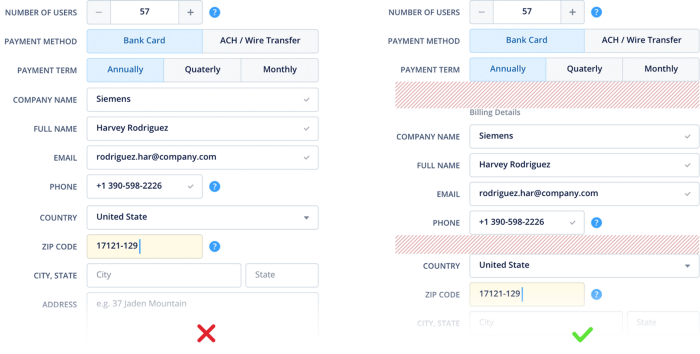
\includegraphics[scale=0.45]{figs/usabilidadeBoaRuim.png}
	\end{center}
	\caption{\label{Formulários}Exemplo de formulários mal elaborados ou confusos.}
    \legend{Fonte: \href{https://i.pinimg.com/564x/5d/66/ce/5d66ce69f103e876c90ab8076c433494.jpg}{https://i.pinimg.com/564x/5d/66/ce/5d66ce69f103e876c90ab8076c433494.jpg}}
\end{figure}

Seja na Web ou em dispositivos móveis, a usabilidade é um conceito importante a se ter em mente ao projetar uma interface, porque se os usuários utilizarem um sistema com baixa usabilidade, não vão querer interagir com ele por muito tempo. Se o aplicativo for complicado de usar, difícil de se obter informações ou se o usuário apenas sentir que está perdido no aplicativo, ele deixará de usá-lo. Claro que existem outros aplicativos para substituí-lo, então o usuário não se preocupará em tentar interagir com sistemas incompreensíveis, e terá medo de cometer erros onde quer que esteja, o que não o deixará confortável e causará estresse e insegurança numa situação que deveria ser simples e intuitiva.

Sendo assim, é considerável que na fase inicial do projeto de qualquer sistema seja feita uma avaliação de usabilidade, não só porque o custo de alterar e melhorar o design é pouco elevado numa fase inicial de desenvolvimento do que após o lançamento no mercado, mas também porque deve-se colocar no mercado uma aplicação útil e com boa usabilidade e que qualquer pessoa consiga facilmente utilizar.

\section{Técnicas de Avaliação da Usabilidade}
\label{Técnicas_de_Avaliação_da_Usabilidade}

Existem vários métodos para estudar e avaliar a usabilidade, porém o mais comum e mais utilizado é o teste com usuários \cite{nielsen-usabilidade}.

Este teste é realizado reunindo um grupo de usuários que possuam ou não conhecimento sobre a aplicação. Este usuários realiza, individualmente, um conjunto de tarefas pré-definidas pela equipe de desenvolvimento da aplicação que, por padrão, correspondem às funcionalidades principais que se quer que a aplicação tenha.

Durante esta etapa, deve-se observar as reações dos usuários durante a interação com a interface e pedir que estes apontem as dificuldades que estão tendo sem nunca interferir no processo, isto é, caso o usuário tenha alguma dúvida sobre como realizar determinada tarefa e questionar sobre isso, somente ao final poderá ser respondida, pois pode-se influenciar e contaminar o resultado do teste, uma vez que já se sabe a resposta e se está testando se o que foi feito é perceptível.

Se para os usuários, realizar essa determinada tarefa não é algo óbvio e intuitivo, então encontrou-se um problema de usabilidade.

Através das dificuldades e problemas apontados pelos usuários, obtém-se soluções para os mesmos e volta-se a realizar testes com novos usuários para filtrar e encontrar novos os problemas de usabilidade.

\subsection{Avaliação Participativa da Usabilidade}
\label{Avaliação_Participativa_da_Usabilidade}

No âmbito deste estudo, a avaliação participativa desempenha um papel crucial na busca por aprimoramentos significativos na interface da plataforma DebugandoED. Diferenciando-se de abordagens tradicionais que dependem exclusivamente de especialistas em usabilidade, nossa metodologia incorpora diretamente as perspectivas dos usuários finais. Este enfoque participativo, centrado na experiência do usuário, visa proporcionar uma avaliação mais alinhada às necessidades reais dos utilizadores.

\section{Comunicabilidade}
\label{Comunicabilidade}
A interface é uma “mensagem” do desenvolvedor/designer para os usuários, com o objetivo de comunicar a quem se destina o sistema, como funciona ou para que serve, quais as vantagens de utilizá-lo e como o usuário deve interagir com o sistema para atingir seus objetivos. Logo, a comunicabilidade destas interfaces são de extrema importância para o usuário entender o funcionamento do sistema \cite{normanDAODESIGNDODIA}

Em sistemas com alta comunicabilidade, os usuários são capazes de responder perguntas como:
\begin{itemize}
    \item Para que o sistema serve?
    \item Qual é a vantagem de utilizá-lo?
    \item Como funciona?
    \item Quais são os princípios gerais de interação com o sistema?
\end{itemize}

O designer deve assegurar que o usuário possa prever e compreender por si só a maneira de utilizar as ferramentas do sistema para realizar as suas atividades com facilidade e eficiência. Caso bem sucedido, o sistema responderá às ações do usuário informando o que está acontecendo, evitando que haja conflitos na interação e, consequentemente, a insatisfação do usuário. Porém, além dessa problemática enfrentada pelo designer, a usabilidade e a comunicabilidade sofrem interferência de outro conceito importante, principalmente em websites, a acessibilidade. 

\section{Acessibilidade}
\label{Acessibilidade}

 \begin{citacao}
 “Acessibilidade é projetar produtos para que pessoas com deficiência possam usá-los. A acessibilidade torna as interfaces de usuário perceptíveis, operáveis e compreensíveis por pessoas com uma ampla gama de habilidades e pessoas em uma ampla gama de circunstâncias, ambientes e condições. Assim, a acessibilidade também beneficia pessoas sem deficiência e organizações que desenvolvem produtos acessíveis” \cite{slhjustask}.
\end{citacao}

A acessibilidade é uma subclasse da usabilidade. Enquanto a usabilidade se preocupa com o universo de todos os potenciais usuários de um sistema, a acessibilidade procura que todas e quaisquer pessoas, independentemente de eventuais limitações sensoriais ou motoras, o possam utilizar. A acessibilidade pretende, com isso, tornar as interfaces perceptíveis e compreensíveis por pessoas em várias circunstâncias, ambientes e condições. A acessibilidade pode ser comparada ao conceito matemático de simetria, segundo o qual algo mantêm as suas características principais depois de submetido a um conjunto de transformações, visto que essas transformações não alteram o objeto ou a sua aparência \cite{matos2021estudo} .
 
\section{Experiência de Usuário}
\label{Experiência_de_Usuário}

O design experimental é o processo de melhoria da \acf{UX}. Visa tornar o produto útil, localizável e acessível, a interface é fácil de usar, desejável e a informação veiculada é confiável. De acordo com \citeonline{brito2016usabilidade}, esse processo geralmente é dividido em três etapas:

\begin{enumerate}
    \item \textbf{\ac{UCD}}: fase de pesquisa durante a qual se analisa e se prevê como os usuários utilizarão os produtos. Nesta fase, os seguintes métodos são utilizados para estudar como os usuários percebem, pensam e tomam decisões:
    \begin{itemize}
        \item Análise Competitiva: Pesquisar produtos competitivos e avaliar sua interface e usabilidade. 
        \item Personas: Criar personagens fictícios para ajudar designers a compreender as necessidades dos usuários finais. 
        \item Fluxo de Usuário: diagrama que representa a rota do usuário ao realizar determinadas tarefas. 
    \end{itemize}
   \item \textbf{Usar as informações obtidas na etapa anterior} para executar:
    \begin{itemize}
        \item \textit{Wireframe}: diagrama de baixa fidelidade que representa o layout de um site ou aplicativo. Este permite que se explore e teste ideias de design em projetos iniciais. 
        \item Ensaio: simulação das ações e pensamentos do usuário conforme se avança no \textit{wireframe} passo a passo.
    \end{itemize}
   \item \textbf{Coleta de \textit{feedback} e teste de usabilidade}: Após a fase de \textit{design}, aparece a etapa de coleta de \textit{feedback} da equipe de produto e clientes, também se passa a fazer testes de usabilidade com os usuários, o que auxilia na correção de problemas de usabilidade do aplicativo.
\end{enumerate}

\section{Design de Interfaces}
\label{Design de Interfaces (UI)}

De acordo com \citeonline{maia2016designui}, a \acf{UI} é o recurso que impulsiona a interação humana com produtos físicos ou virtuais. A interface varia de brinquedos e eletrodomésticos a aplicativos móveis ou páginas da web. O trabalho de um designer de interface não se limita a compreender os problemas e necessidades do usuário. Este tipo de projeto envolve conhecimento técnico e estético da construção de ferramentas funcionais. Na prática, o design da interface envolve: partes visuais, usabilidade, arquitetura da informação, navegação e transições de tela. Em outras palavras, todas as funções que aumentam e melhoram a maneira como os usuários lidam com os produtos. Tudo deve ser construído pela satisfação dos fatores humanos. Nesse sentido, a \acf{UX} deve ser o foco de atenção no desenvolvimento de produtos, serviços ou sistemas. Um bom projeto, não importa o quão grande ou pequeno seja, deve passar por um estágio de ideias e necessidades esperadas dos usuários.

A interface bem projetada é principalmente responsável por permitir que os usuários naveguem em sites ou aplicativos. Incentivar e fidelizar esse usuário também é uma meta. Portanto, quando bem pensada, a interface tem a capacidade de se tornar uma ferramenta e facilitar a vida das pessoas. Ignorar a importância do design da interface pode ser o fator decisivo na rejeição de aplicativos. Em suma, o que é importante para os usuários é que o sistema seja fácil de usar e que possa cumprir sua função de criação. Por exemplo, quando alguém usa um aplicativo bancário, deseja que o aplicativo execute a transação principal, evitando assim ir à agência. Portanto, o objetivo do design de interface é ajudar a criar ferramentas atraentes, úteis e eficazes para a solução de problemas \cite{maia2016designui}.

\section{Heurísticas de Jakob Nielsen}
\label{Heurísticas de Jakob Nielsen}

Em 1990, Jakob Nielsen\footnote{em \url{https://www.nngroup.com/people/jakob-nielsen/} está a biografia de Jakob Nielsen e todos os seus trabalhos.} propôs 10 heurísticas que devem ser consideradas ao desenvolver qualquer interface. Nesse caso, as heurísticas referem-se ao senso comum que visa reduzir a sobrecarga cognitiva dos usuários. Portanto, pode tornar a navegação, viagem e experiência melhores, além de reduzir o cansaço. 

Diz-se que as heurísticas de \citeonline{nielsen2005ten} são regras gerais porque não podem determinar diretrizes específicas para usabilidade ou desenvolvimento de interface. Nesse sentido, o método heurístico está relacionado aos anos de experiência e conhecimento do autor.

Com isso, as heurísticas de \citeonline{nielsen2005ten} são:
\begin{enumerate}
    \item \textbf{Visibilidade do status do sistema}: O sistema deve sempre manter os usuários informados sobre o que está acontecendo, por meio de \textit{feedback} apropriado dentro de um período de tempo razoável.
    \item \textbf{Correspondência entre o sistema e o mundo real}: A interface deve ser funcional e acessível que fale a linguagem dos usuários, usando palavras, frases e conceitos familiares ao usuário, em vez de termos técnicos.
    \item \textbf{Liberdade e controle do usuário}: Os usuários geralmente agem por engano, eles precisam de uma ''saída de emergência'' claramente marcada para que ações desnecessárias possam ser deixadas, sem a realização de procedimentos complicados.
    \item \textbf{Consistência e padrões}: Os usuários não devem se perguntar se palavras, situações ou ações diferentes significam a mesma coisa. Siga as práticas da plataforma e do setor. 
    \item \textbf{Prevenção de erros}: Boas mensagens de erro são importantes, porém o melhor design evitará problemas. Elimine condições sujeitas a erros ou conduza inspeções e forneça aos usuários opções de confirmação antes de submeter à operação.
    \item \textbf{Reconhecer ao invés de lembrar}: Minimize a carga de memória do usuário, o usuário não precisa se lembrar de informações de uma parte da interface para outra. As informações necessárias para usar a interface (por exemplo, rótulos de campo ou itens de menu) devem ser visíveis ou facilmente recuperadas quando necessário.
    \item \textbf{Flexibilidade e Eficiência}: Atalhos que não são bem conhecidos por novatos podem acelerar a interação de usuários experientes, de modo que a interface possa servir tanto a usuários inexperientes quanto experientes.
    \item \textbf{Estética e Design minimalista}: A interface não deve conter informações irrelevantes ou raramente necessárias. Cada unidade de informação adicional na interface competirá com a unidade de informação relevante, reduzindo assim sua visibilidade relativa.
    \item \textbf{Auxiliar usuários a reconhecer, diagnosticar e recuperar erros}: A mensagem de erro deve ser expressa em linguagem simples (sem código de erro), apontar o problema com precisão e propor uma solução de forma construtiva. 
    \item \textbf{Ajuda e Documentação}: De preferência, o sistema não requer nenhuma explicação adicional. No entanto, pode ser necessário fornecer documentação para ajudar os usuários a entenderem como realizar suas tarefas.
\end{enumerate}

\section{Gestalt}
\label{Princípios de Gestalt}
O estudo da Gestalt está relacionado à percepção que os usuários vêm do mundo e o que nele contém. Ele explica como o cérebro pode influenciar em determinadas situações, através da interpretação do que se vê \cite{gestalt7principios}.

Ao tentar entender o que nos rodeia, o que a Gestalt sugere é que não se concentre em cada componente pequeno, mas sim em como eles interagem uns com os outros, em sistemas complexos. O princípio da Gestalt desempenha, por isso, um papel importante no desenvolvimento moderno do estudo da sensação e da percepção humana, no design e na publicidade \cite{gestaltleticiasimoes}.

\subsection{Princípios da Gestalt}

Para melhor se trabalhar a Gestalt, seus princípios foram separados em 7:

\begin{enumerate}
    \item \textbf{Princípio da Proximidade:}
    
    Objetos que estão próximos uns aos outros são percebidos, segundo o princípio da proximidade, como mais relacionados do que objetos mais separados. A proximidade diz que quando elementos são posicionados um perto do outro eles são vistos como parte de um grupo, e não individualmente. Eles não precisam sequer ser parecidos, o mero fato de dividirem o mesmo espaço é o suficiente para a proximidade funcionar.
    
    \begin{itemize}
        \item Aplicação na Design \ac{UI}
        
        Assim, algumas das diversas aplicações deste princípio dentro de \ac{UI} se encontram na forma que elementos diferentes são posicionados de forma próxima para formar um grupo.
        
        Na \autoref{proximidade}, os labels estão próximos aos campos para que sejam percebidos como uma coisa só:
        
        \begin{figure}[htb]
        	\begin{center}
        	    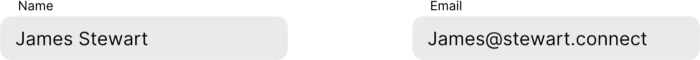
\includegraphics[scale=0.45]{figs/proximidade.png}
        	\end{center}
        	\caption{\label{proximidade}Exemplo de Proximidade}
            \legend{Fonte: \href{https://miro.medium.com/v2/resize:fit:720/0*db8wjIe_ZFTqD4uS}{https://miro.medium.com/v2/resize:fit:720/0*db8wjIe\_ZFTqD4uS}}
        \end{figure}
    \end{itemize}

    \item \textbf{Princípio da Similaridade:}
    
    Usuários percebem objetos que parecem semelhantes como tendo usos semelhantes. Essa é uma estratégia simples que você pode usar em seus designs como meio para comunicar a função de um determinado objeto rapidamente, aumentando a usabilidade.
    
    Ao criar ícones ou estruturas similares, por exemplo, se economiza muito tempo explicando para o usuário qual é a sua função.
    
    \begin{itemize}
        \item Aplicação
        
        Na \autoref{similaridade}, pode-se perceber que os campos têm a mesma função, mas que o botão, apesar de ter forma semelhante, possui outra funcionalidade, já que seu tratamento é diferente.
        
        \begin{figure}[htb]
        	\begin{center}
        	    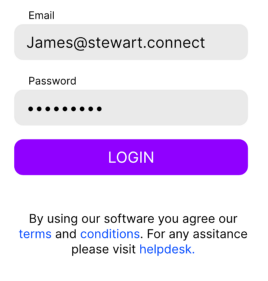
\includegraphics[scale=0.5]{figs/similaridade.png}
        	\end{center}
        	\caption{\label{similaridade}Exemplo de Similaridade}
        	\legend{Fonte: \href{https://miro.medium.com/v2/resize:fit:720/0*yW15A7gQjg6cDsFY}{https://miro.medium.com/v2/resize:fit:720/0*yW15A7gQjg6cDsFY}}
        \end{figure}
    \end{itemize}
    
    \item \textbf{Princípio da Continuidade}
    
    Por mais estranho que isso pareça à primeira vista, o olhar do usuário cria um tipo de impulso à medida que ele se move de objeto para objeto em um layout, e a isso chamamos de continuidade.

    Linhas, em geral, aumentam esse efeito. Tanto que é possível perceber curvas e retas onde elas não existem, apenas pela disposição dos elementos que compõem uma imagem.

    O poder da continuidade se sobrepõe ao poder da cor. Vemos isso aplicado todos os dias nas barras de navegação verticais e horizontais.
    
    \begin{itemize}
        \item Aplicação
        
        Na \autoref{continuidade}, o fato de que o componente de carrossel está cortado nos limites da tela cria esta ilusão e enfatiza a função de se arrastar para ver mais itens.
        
        \begin{figure}[htb]
        	\begin{center}
        	    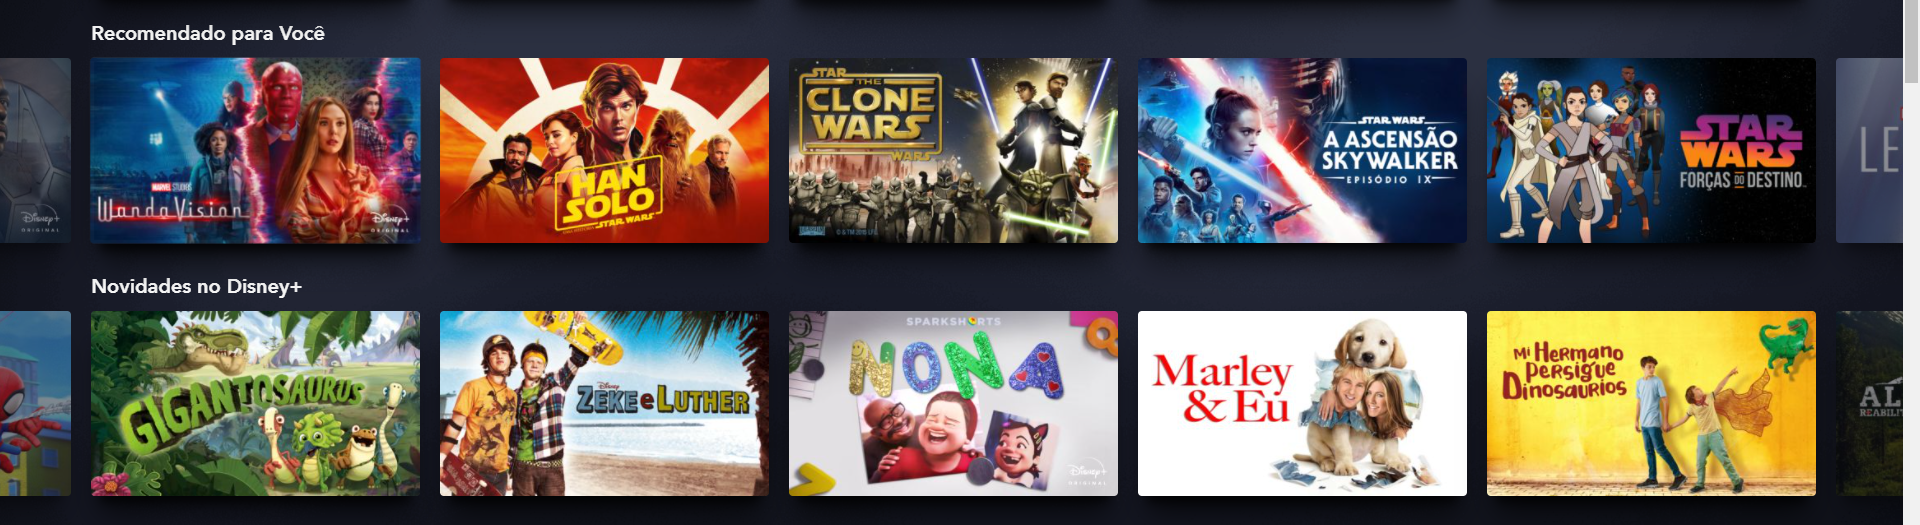
\includegraphics[scale=0.30]{figs/continuidade.png}
        	\end{center}
        	\caption{\label{continuidade}Exemplo de Continuidade}
        	\legend{Fonte: Print da página da Disney Plus \protect\url{https://www.disneyplus.com/}}
        \end{figure}
    \end{itemize}

     \break
    
    \item \textbf{Princípio do Fechamento}
    
    O fechamento, por sua vez, aplica as propriedades mencionadas pelo princípio da Gestalt e faz com que usuários completem objetos na sua mente caso eles estejam parcialmente obscurecidos.

    O minimalismo e o uso de elementos parciais emprega o fechamento para economizar espaço e para se comunicar com eficiência.
    
    \begin{itemize}
        \item Aplicação
        
        Na \autoref{fechamento}, a forma com que os elementos são agrupados (utilizando todos os princípios já citados até aqui) cria grupos fechados em si mesmos, mesmo sem que precisemos contornar ou demarcar as seções.
        
        \begin{figure}[htb]
        	\begin{center}
        	    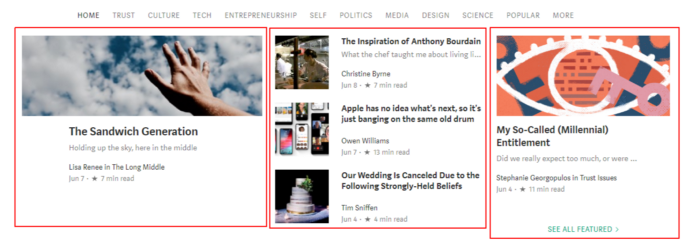
\includegraphics[scale=0.45]{figs/fechamento.png}
        	\end{center}
        	\caption{\label{fechamento}Exemplo de Fechamento}
        	\legend{Fonte: \href{https://miro.medium.com/v2/resize:fit:720/0*43pZlU1PtSsY4AZF}{https://miro.medium.com/v2/resize:fit:720/0*43pZlU1PtSsY4AZF}}
        \end{figure}
    \end{itemize}
    
    \item \textbf{Princípio da Figura-Fundo}
    
    Este princípio afirma que nossa percepção instintivamente percebe objetos como estando à frente ou ao fundo. Pois, como seres humanos, não somos capazes de focar na frente e no fundo simultaneamente, e precisamos escolher apenas um.
    
    \begin{itemize}
        \item Aplicação
        
        Assim, em interfaces, este princípio é amplamente aplicado em navegações, modais e caixas de diálogo. Pode ser observado na \autoref{figura-fundo} que o fundo torna-se secundário quando uma ação que necessita de maior foco é trazida à frente:
        
        \begin{figure}[htb]
        	\begin{center}
        	    \includegraphics[scale=0.45]{figs/figura-fundo.png}
        	\end{center}
        	\caption{\label{figura-fundo}Exemplo de Figura-fundo}
            \legend{Fonte: \href{https://miro.medium.com/v2/resize:fit:720/0*Xb_zAcb44hjXitEa}{https://miro.medium.com/v2/resize:fit:720/0*Xb\_zAcb44hjXitEa}}
        \end{figure}
    \end{itemize}
    
    \item \textbf{Princípio da Região Comum}
    
    O princípio da região comum têm relação com princípio da proximidade, podendo ser até mesmo considerado um sub-princípio deste primeiro. Dessa forma, esse principio afirma que quando objetos são posicionados dentro da mesma região fechada estes são percebidos como parte do mesmo grupo.
    
    \begin{itemize}
        \item Aplicação
        
         Na \autoref{Região Comum} este princípio é amplamente encontrado através da utilização de cards, pois estes criam regiões isoladas de informação, mesmo quando existem diversos cards próximos uns aos outros.
        
        \begin{figure}[htb]
        	\begin{center}
        	    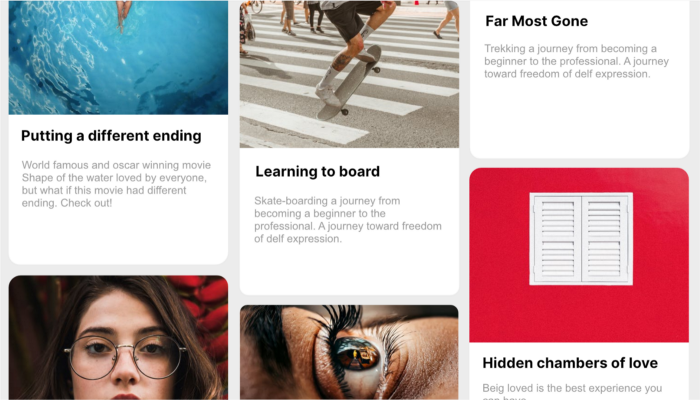
\includegraphics[scale=0.45]{figs/regiao-comum.png}
        	\end{center}
        	\caption{\label{Região Comum}Exemplo de Região Comum}
            \legend{Fonte: \href{https://miro.medium.com/v2/resize:fit:720/0*6SjBY8cq3i95lf_d}{https://miro.medium.com/v2/resize:fit:720/0*6SjBY8cq3i95lf\_d}}
        \end{figure}
    \end{itemize}
    \newpage
    
    \item \textbf{Princípio do Ponto Focal}
    
    O princípio do ponto focal afirma que qualquer elemento que se destacar visualmente vai capturar e prender a atenção de quem está vendo.
    
    \begin{itemize}
        \item Aplicação
        
         Na \autoref{ponto focal} percebe-se que quando é selecionada a parte do corpo, esta se torna em ponto focal. E ao mesmo tempo, o botão verde deixa claro qual é a próxima ação a ser executada
        
        \begin{figure}[htb]
        	\begin{center}
        	    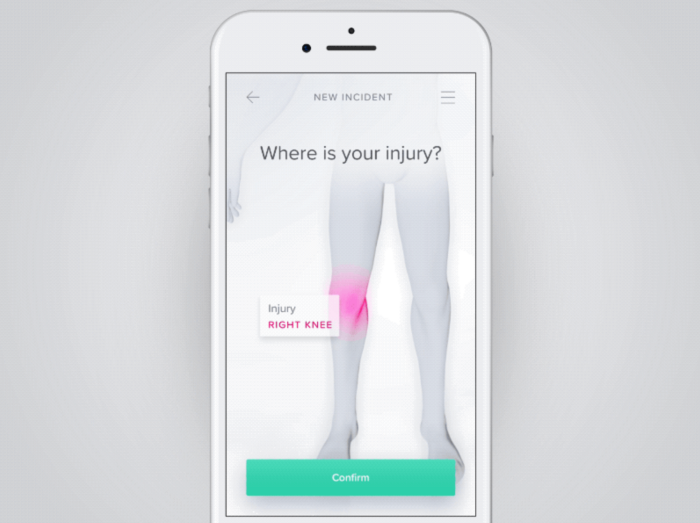
\includegraphics[scale=0.35]{figs/ponto-foca.png}
        	\end{center}
        	\caption{\label{ponto focal}Exemplo de Ponto Focal}
        	\legend{Fonte: \href{https://miro.medium.com/max/700/0*GawJYiOzuiRKBbgq.png}{https://miro.medium.com/max/700/0*GawJYiOzuiRKBbgq.png}}
        \end{figure}
    \end{itemize}
\end{enumerate}


\section{\textit{Material Design}}
\label{Material_Design}

\textit{Material Design} é um conceito visual apresentado pela Google em sua conferência anual que ocorreu em 25 de junho de 2014, a Google I/O\footnote{\url{https://io.google}}.

De acordo com a interpretação de \citeonline{rodrigues2017aplicaccao}, o \textit{Material Design\footnote{\url{https://material.io/}}} é inspirado em materiais e objetos do mundo real, que reagem de acordo como são manuseados, e vem com várias sugestões para melhorar a experiência da interface do usuário, propondo simplicidade e naturalidade na utilização dos mais diversos tipos de sistemas operacionais.

As principais propostas funcionais deste conceito são os efeitos de animações e transições expressivas, seja de telas inteiras ou objetos, além de efeitos de profundidade, iluminação e sombras realistas, dando a impressão de naturalidade, tornando assim algo virtual tão simples a ponto de fazer o usuário sentir que está fazendo algo extremamente comum e cotidiano sem grande esforço mental.

Para \citeonline{CordeiroFilipeIMD}, a Google tem como intenção desenvolver uma forma única de design que permite ao usuário ter a mesma experiência em todas as plataformas e enumerou 3 conceitos importantes:

\begin{enumerate}
    \item \textbf{O Material é a Metáfora:} O material é baseado na realidade tátil, inspirado no estudo do papel e da tinta, mas tecnologicamente avançado e aberto à imaginação do desenvolvedor. Superfícies e bordas são a prova visual de que tudo é baseado na realidade.
    \item \textbf{Ousado, Gráfico e Intencional:} Os elementos essenciais do design baseado em impressão são: tipografia, grades, espaço, escala, cor e o uso de imagens principais. Esses elementos são mais do que agradáveis aos olhos. Eles criam hierarquia, significado e foco. Opções de cores, aparência de ponta a ponta, tipografia grande e espaço em branco intencional criam uma interface gráfica arrojada.
    \item \textbf{Movimento Fornece Significado:} O movimento respeita e reforça o usuário como motor principal. A ação primária do usuário é o ponto que inicia o movimento. Todas as ações ocorrem dentro de um único ambiente, e os objetos são apresentados ao usuário sem interromper a continuidade da experiência, mesmo quando eles mudam e se reorganizam. O movimento é significativo e apropriado, ajuda a focar e manter a continuidade. O \textit{feedback} é sutil, mas claro. As transições são eficazes e claras.
\end{enumerate}
		
	
	% ----------------------------------------------------------
	% Experimentos e avaliação dos resultados
	% Obrigatório somente para TCC 2
	% ----------------------------------------------------------
	\chapter[Experimentos, Análises e Resultados]{Experimentos, Análises e Resultados}
\label{capExperimentos}

Este capítulo fará uma análise baseada em \acs{UX} e \acs{UI} da Plataforma \href{https://debugandoed.facom.ufu.br/}{DebugandoED}. Este capítulo está organizado da seguinte forma: A seção \ref{secDebugandoED} descreve a plataforma \href{https://debugandoed.facom.ufu.br/}{DebugandoED} utilizado no redesign. Na sequência, a seção \ref{secMetodologia} descreve a metodologia utilizada para o desenvolvimento do redesign da interface e a coleta de percepções dos participantes. A seção \ref{secExperimentos} apresentará os detalhes do experimento a ser realizado, delineando a base dos estudos, o menu de navegação, o conteúdo na página inicial, os campos de entrada de dados, o formulário de cadastro, o formulário de login e o conteúdo das telas de simulação. Por fim, a seção \ref{secAnálisePropostasExperimento} apresenta a análise das propostas por experimento, incluindo pesquisas de opinião realizadas tanto com estudantes \ref{Pesquisa_de_Opinião_com_Estudantes} quanto com profissionais \ref{Pesquisa_de_Opinião_com_Profissionais}, fornecendo uma visão abrangente dos resultados alcançados ao longo deste capítulo.

\section{DebugandoED}
\label{secDebugandoED}

A plataforma \href{https://debugandoed.facom.ufu.br/}{DebugandoED} foi desenvolvida por \citeonline{debugandoedsbsi} e representa um esforço inovador para criar uma ferramenta educacional interativa, centrada na simulação de conceitos fundamentais de programação e estrutura de dados. Ao reconhecer a demanda por abordagens pedagógicas mais eficazes, o projeto concentrou-se em desenvolver um simulador acessível por meio de uma plataforma web, proporcionando aos alunos uma experiência prática e dinâmica \cite{debugandoedsbsi}.

O site, acessível por meio do endereço \href{https://debugandoed.facom.ufu.br}{https://debugandoed.facom.ufu.br}, foi concebido após um estudo aprofundado envolvendo professores de programação e estrutura de dados. O objetivo inicial foi identificar as principais dificuldades enfrentadas pelos alunos nesses cursos. O resultado desse estudo direcionou o desenvolvimento do simulador, com foco nas estruturas básicas de programação, como vetor, matriz, ponteiro, pilha, fila, e listas.

Ao contrário de muitos simuladores disponíveis na literatura, o \href{https://debugandoed.facom.ufu.br/}{DebugandoED} vai além da simples representação visual de interações. Ele oferece aos usuários a capacidade de observar não apenas o resultado visível, mas também os comandos executados e as mudanças na memória. Essa abordagem única visa proporcionar uma compreensão mais profunda dos conceitos, permitindo que os usuários realizem “\textit{debug}” de estruturas sem a necessidade de \ac{IDE} ou conhecimentos avançados de programação.

\section{Metodologia}
\label{secMetodologia}

A metodologia adotada para o desenvolvimento do redesign da interface da plataforma \href{https://debugandoed.facom.ufu.br/}{DebugandoED} e a coleta de percepções de estudantes e profissionais baseia-se em uma abordagem prática e participativa. As etapas do processo envolvem a utilização da ferramenta Figma\footnote{\url{https://www.figma.com/}} para a criação das imagens do redesign da interface, permitindo a prototipagem e visualização das propostas de forma interativa e colaborativa. Além disso, os questionários para coleta de percepções são elaborados e aplicados por meio da plataforma Google Forms\footnote{\url{https://docs.google.com/forms}}.


\subsection{Desenvolvimento de Protótipos}

Neste estágio, são criadas imagens do redesign da interface da plataforma \href{https://debugandoed.facom.ufu.br/}{DebugandoED} utilizando a ferramenta Figma. A utilização do Figma permite a criação de imagens estáticas das propostas de redesign, possibilitando a visualização e avaliação das diferentes telas e fluxos de navegação. A criação de imagens viabiliza a aplicação prática dos conceitos teóricos de usabilidade, comunicabilidade, acessibilidade, \ac{UX} e \ac{UI}, permitindo a avaliação e refinamento das propostas de design com base na análise das imagens simuladas.

\subsection{Coleta de Percepções}

Para a coleta de percepções de estudantes e profissionais sobre o redesign da interface, são elaborados questionários estruturados utilizando a plataforma Google Forms. Os questionários abrangem aspectos relevantes relacionados à usabilidade, acessibilidade,  \ac{UX} e \ac{UI} na interface da plataforma \href{https://debugandoed.facom.ufu.br/}{DebugandoED}. A escolha pelo Google Forms como plataforma para a aplicação dos questionários proporciona facilidade na coleta, organização e análise dos dados obtidos, contribuindo para a compreensão das percepções dos participantes.

\subsubsection{Preocupações Éticas}

Durante a coleta de percepções de estudantes e profissionais sobre o redesign da interface da plataforma \href{https://debugandoed.facom.ufu.br/}{DebugandoED}, são consideradas preocupações éticas relacionadas à privacidade e confidencialidade dos participantes. Os questionários são elaborados de forma anônima, sem a necessidade de identificação dos participantes, garantindo a proteção dos dados coletados. Além disso, é solicitado o consentimento informado dos participantes antes da aplicação dos questionários, esclarecendo os objetivos da pesquisa e garantindo a livre escolha de participação, assegurando a integridade ética da coleta de percepções.

\section{Experimento}
\label{secExperimentos}

A proposta deste trabalho é aplicar os conceitos e princípios apresentados no \autoref{capFund} à plataforma da \autoref{secDebugandoED}. Não serão abordadas todas as telas da plataforma, pois algumas delas são, basicamente, os mesmos objetos aplicados a uma nova situação. No entanto, foi adotado uma abordagem específica para a análise. Serão analisados: menu de navegação, conteúdos da página inicial, campos de entrada de dados, formulário de cadastro, formulário de login e telas de simulação. Para cada um desses itens, a proposta é realizar uma inspeção de usabilidade, aplicando os conceitos e princípios relevantes e propor modificações que seja condizente com os mesmos.

\subsection{Base dos Estudos}

Conforme já explicitado, a Plataforma da \autoref{secDebugandoED} será utilizada como estudo de caso para a aplicação dos conceitos e princípios apresentados no \autoref{capFund}.  A tela inicial da plataforma pode ser visualizada na \autoref{debugandoED01}. A Plataforma está em constante evolução e está sendo implementada a parte de \textit{gamificação}, com isso, pode ser que algumas telas, com o passar do tempo, possam estar modificadas quando comparadas com as apresentadas neste trabalho.

\begin{figure}[ht]
    \begin{center}
        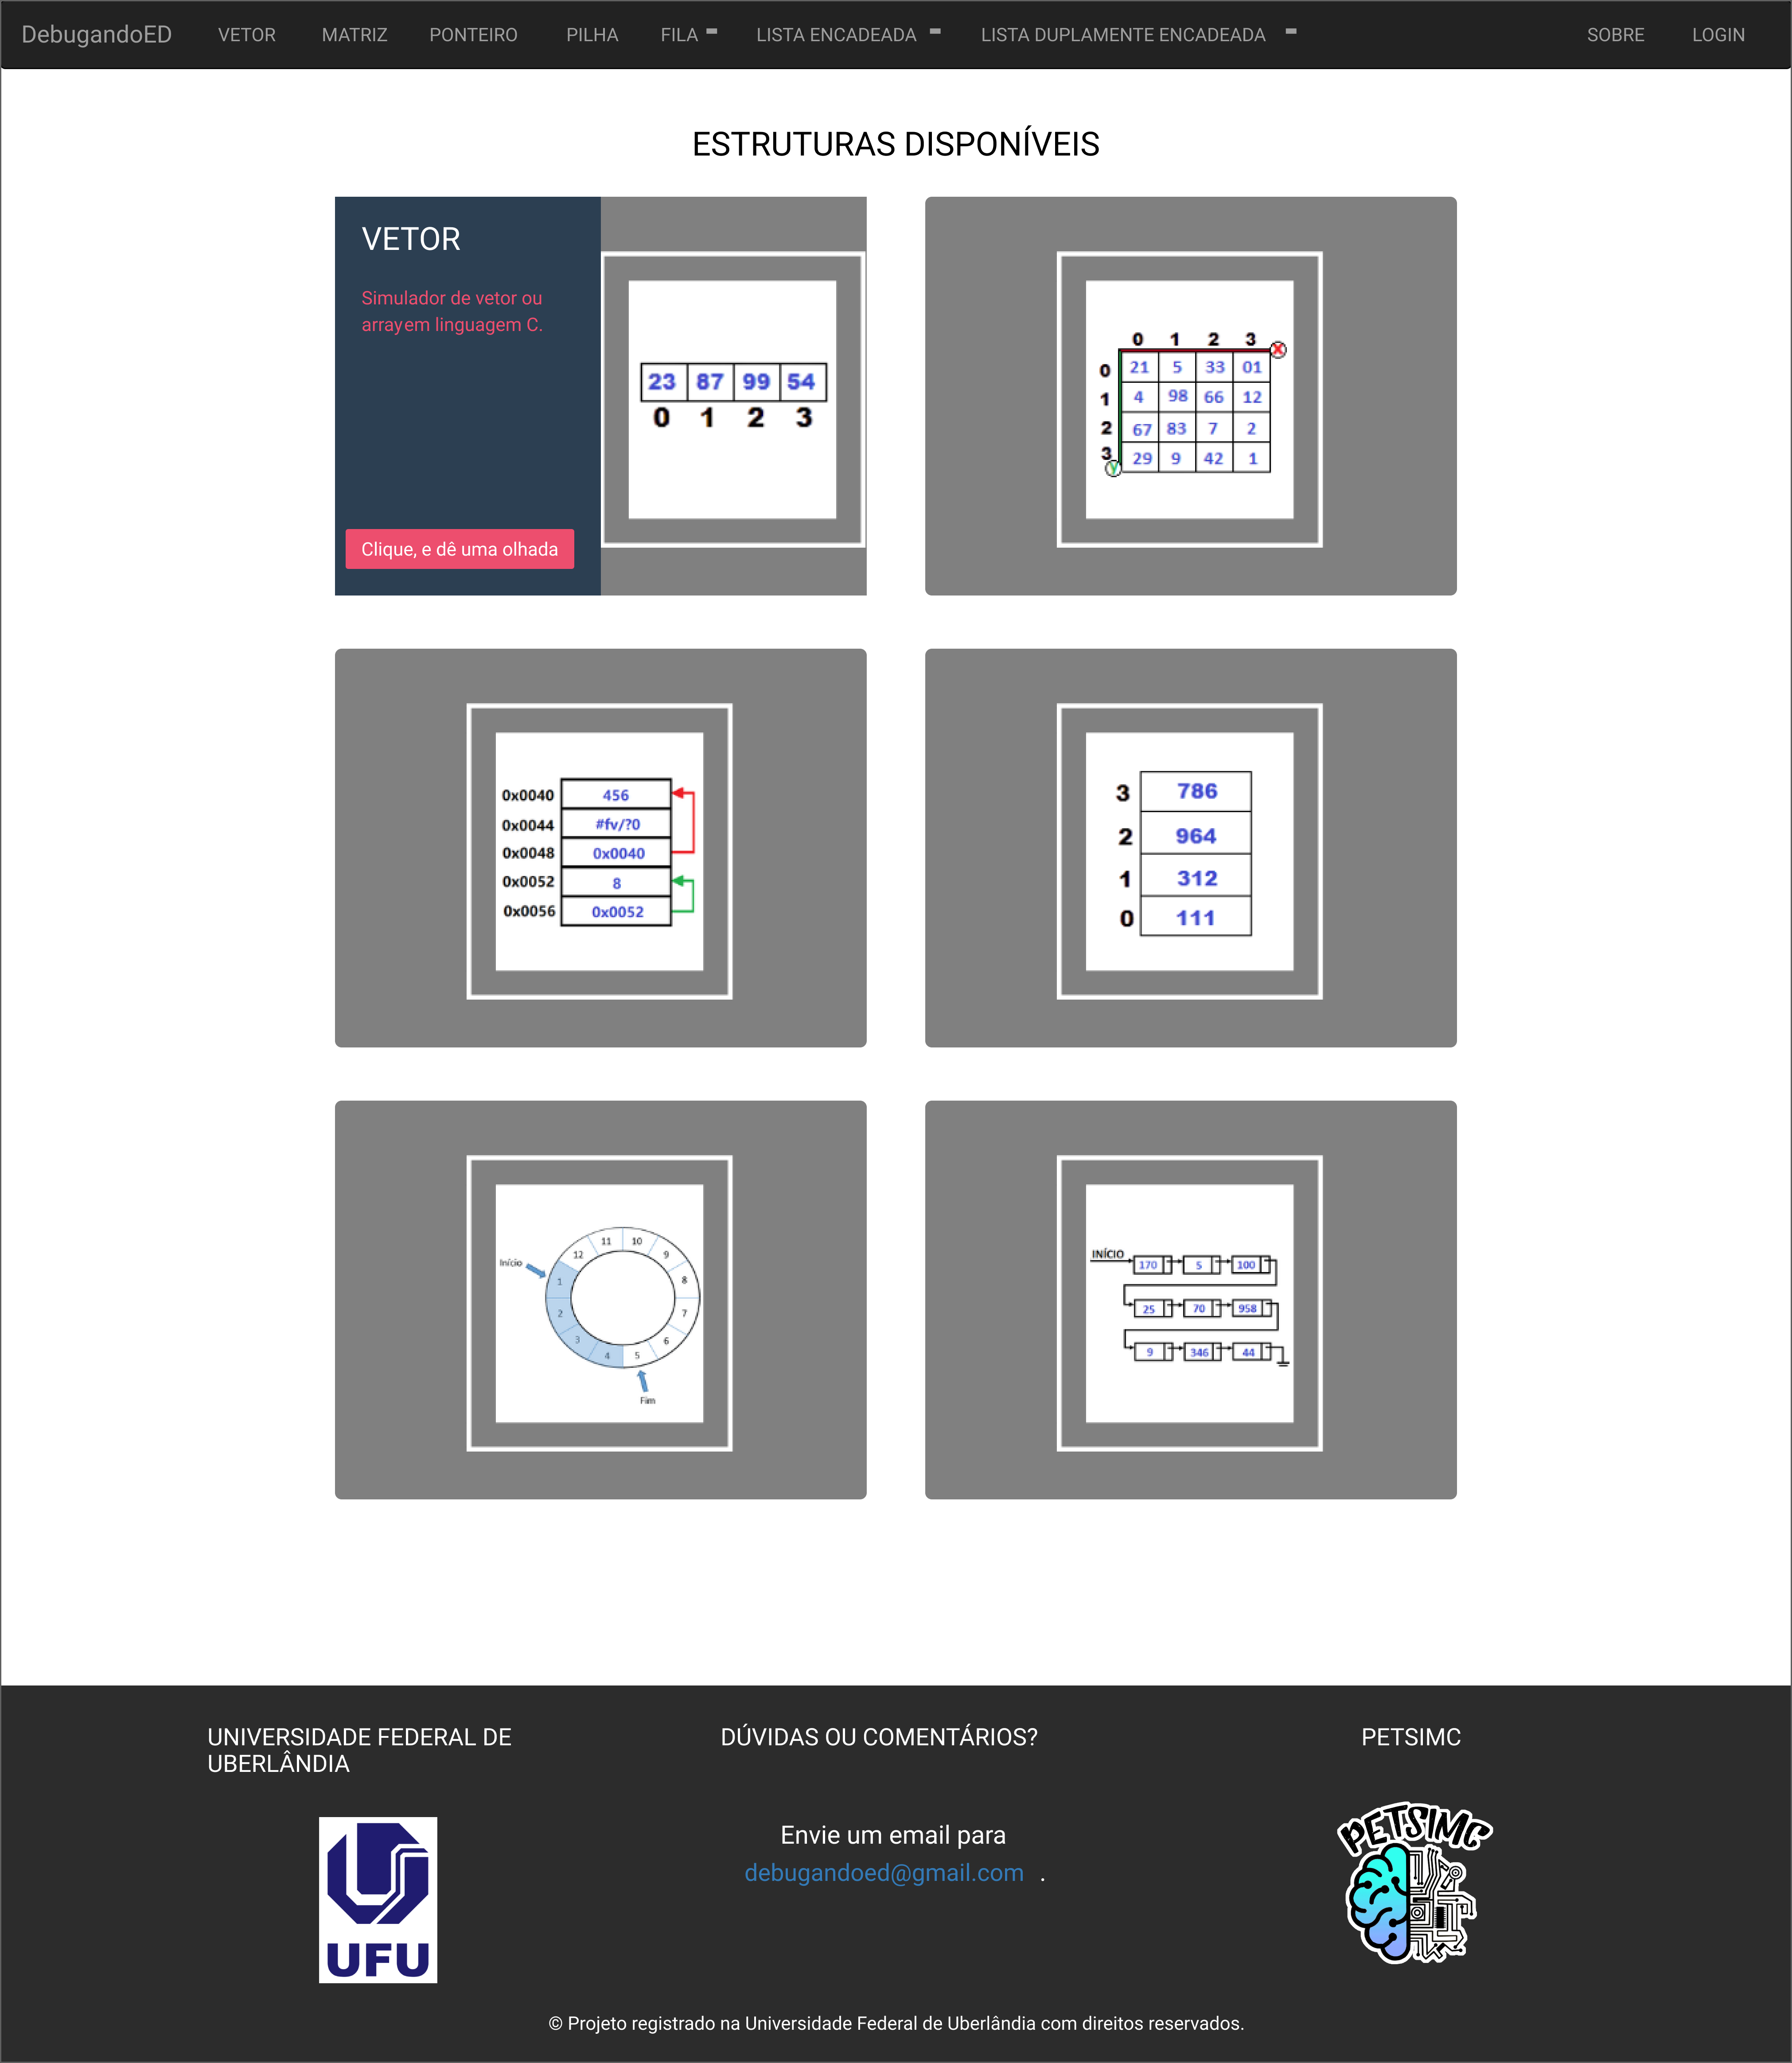
\includegraphics[scale=0.3]{figs/debugandoED01.png}
    \end{center}
    \caption{\label{debugandoED01}Tela inicial da Plataforma DebugandoED.}
    \legend{Fonte: \href{https://debugandoed.facom.ufu.br/}{https://debugandoed.facom.ufu.br}}
\end{figure}


\subsection{Menu de Navegação}
\label{Menu_de_Navegação}

De acordo com o seção de Design de Interfaces (\autoref{Design de Interfaces (UI)}) e a Heurísticas de Estética e Design minimalista de Jakob Nielsen (\autoref{Heurísticas de Jakob Nielsen}), nota-se no menu de opções apresentado na \autoref{debugandoED01}, um desacordo na utilização de cores e contrastes, onde o menu é fundo preto com texto em cor cinza, logo nota-se não haver uma padronização na escala de cores utilizadas.
    
Um simples ajuste de fonte e cor, obtém um contraste melhor e por consequência mais legibilidade, optando-se pelo branco como cor da fonte ao invés do cinza (\autoref{debugandoED-menu} - B) e aumentando o peso da fonte (\autoref{debugandoED-menu} - C).
    
    \begin{figure}[htb]
        \begin{center}
    	    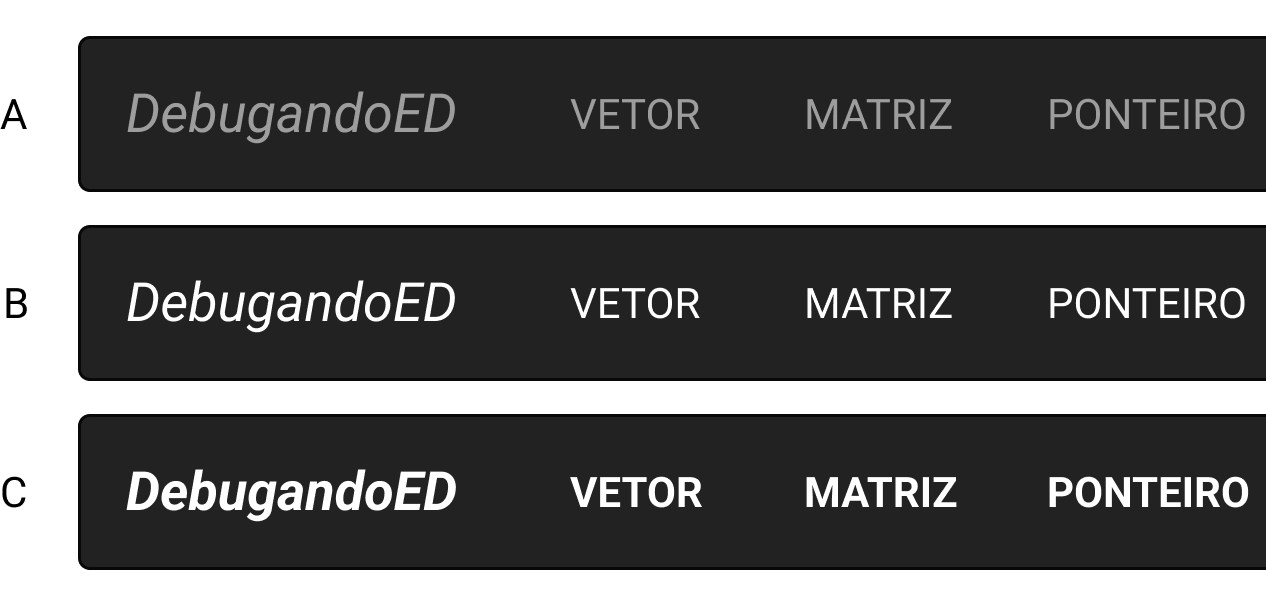
\includegraphics[scale=1]{figs/debugandoED-menu.png}
    	\end{center}
        \caption{\label{debugandoED-menu}Ajustes na fonte do menu: (A) Original; (B) Troca da cor; (C) Aumento do peso da fonte de B.}
    \end{figure}
    
 Outro ponto de Jakob Nielsen, é a heurísticas de reconhecer ao invés de lembrar (\autoref{Heurísticas de Jakob Nielsen}), tornando as abas mais reconhecíveis com ícones, entretanto, em especifico este possui várias abas tornando complexo respeitar o Princípio da Proximidade de Gestalt sendo necessário a utilização de técnicas de responsividade para tela de tamanho diferentes (\autoref{debugandoED-menu-icons}).
 
\begin{figure}[htb]
    \begin{center}
        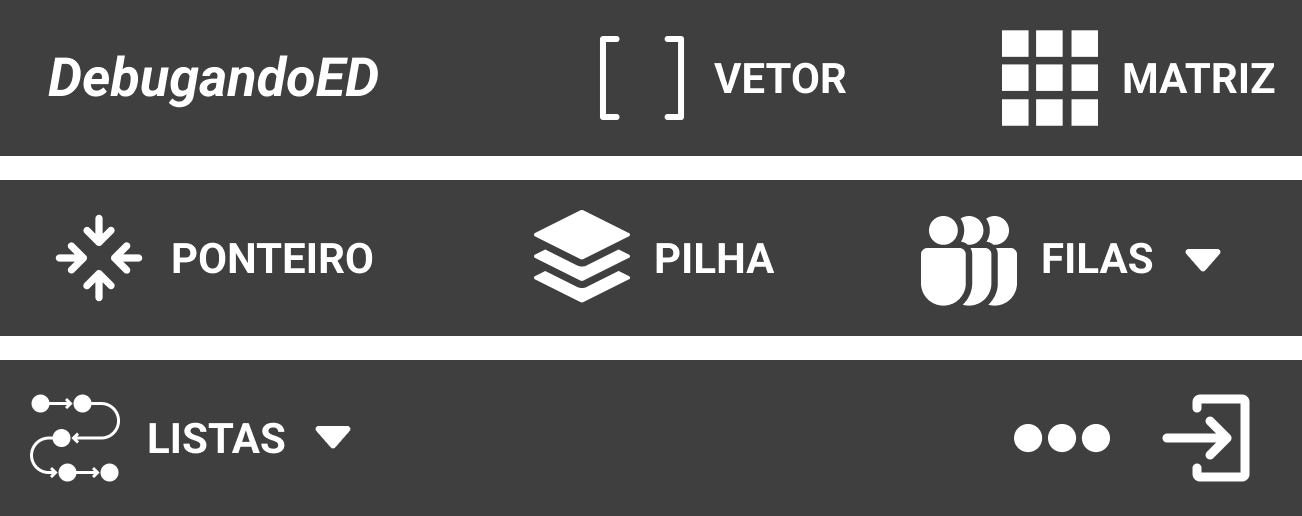
\includegraphics[scale=1]{figs/debugandoED-menu-icons.png}
    \end{center}
    \caption{\label{debugandoED-menu-icons}Proposta de ícones para trabalhar a heurísticas de reconhecer.}
\end{figure}

No conceito da \autoref{Experiência_de_Usuário}, onde é tratado a experiência do usuário, adicionar uma forma visual de localização no menu de navegação na sobreposição do mouse em cima de cada item do menu (\autoref{debugandoED-menu-hovers}), isso apenas localiza o usuário de onde ele está, melhorando sua experiência. A proposta na \autoref{debugandoED-menu-hovers} é um efeito, onde o conteúdo em forma de um botão estivesse se elevando dos demais, logo o destacando.

\begin{figure}[htb]
    \begin{center}
        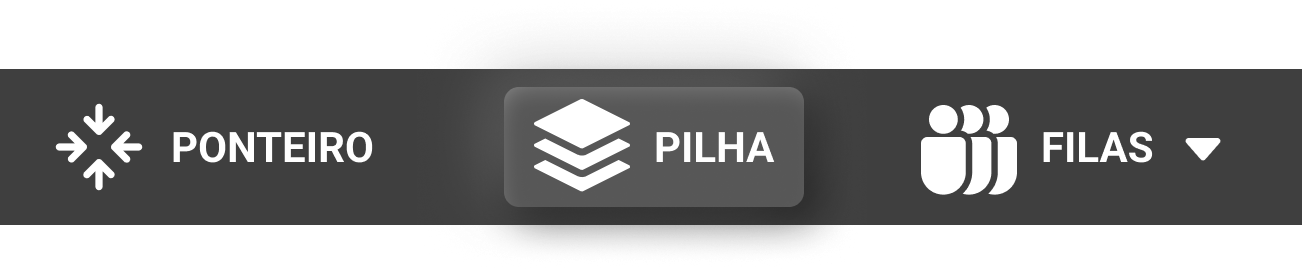
\includegraphics[scale=1]{figs/debugandoED-menu-hover.png}
    \end{center}
    \caption{\label{debugandoED-menu-hovers}Exemplo de destaque para localização do item do menu pelo usuário.}
\end{figure}

\subsection{Conteúdo na Página Inicial}
\label{Conteúdo_na_Pagina_Inicial}

De acordo com a correspondência entre o sistema e o mundo real (\autoref{Heurísticas de Jakob Nielsen}), na \autoref{debugandoED-bloco-antes} pode-se notar um dos diversos blocos que a tela inicial possui, com imagens representando outras funcionalidades específicas da plataforma, imagens não tão simples para usuário leigos no assunto, embora tenha o efeito de sobreposição do mouse no qual é mostrado mais informações sobre aquele bloco, isto pode ser melhorado colocando alguma forma de indicativo ou informação simplificada sem a necessidade de sobrepor o mouse nos blocos.
    
\begin{figure}[htb]
    \begin{center}
	    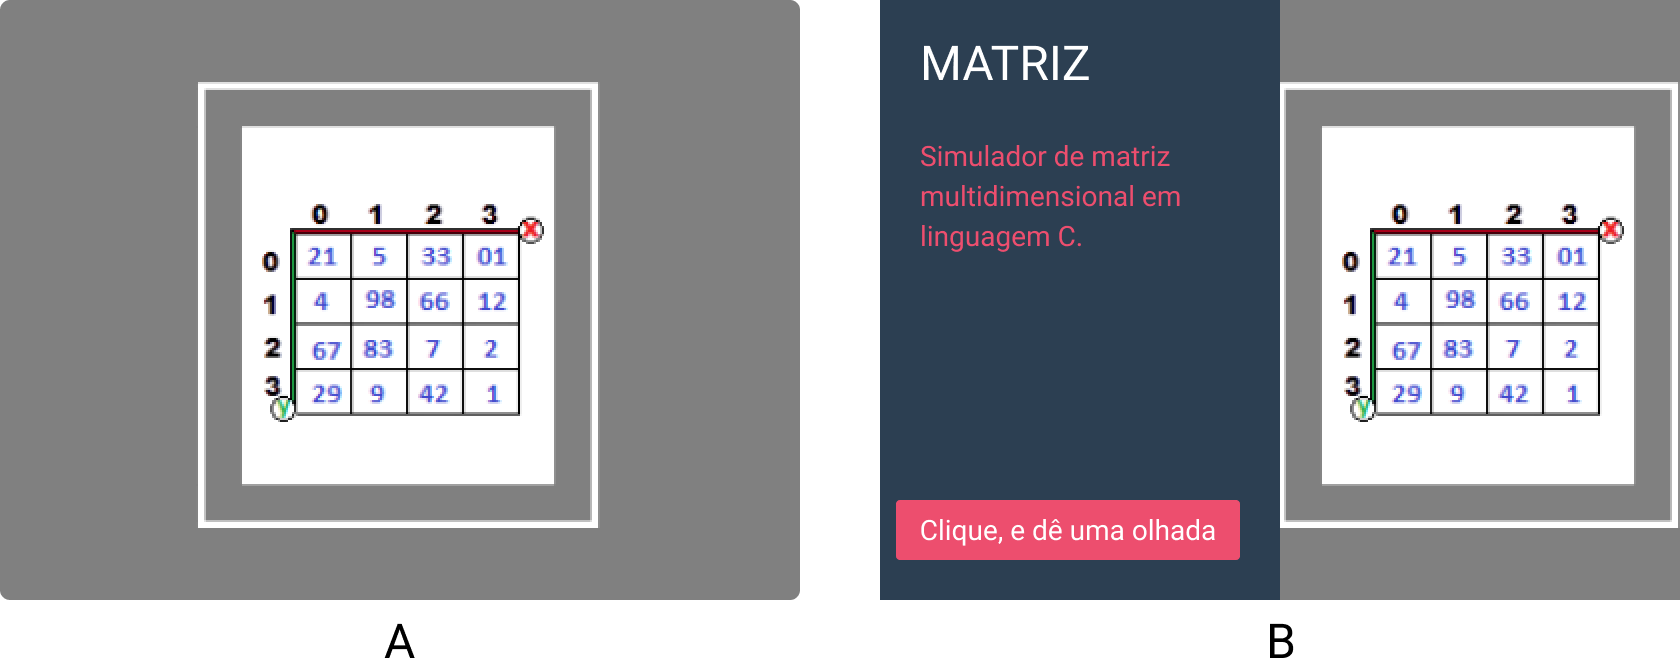
\includegraphics[scale=0.52]{figs/debugandoED-bloco-antes.png}
	\end{center}
    \caption{\label{debugandoED-bloco-antes}Blocos de Matriz (Original): (A) sem sobreposição - (B) com sobreposição.}
\end{figure}
    
\begin{figure}[htb]
    \begin{center}
	    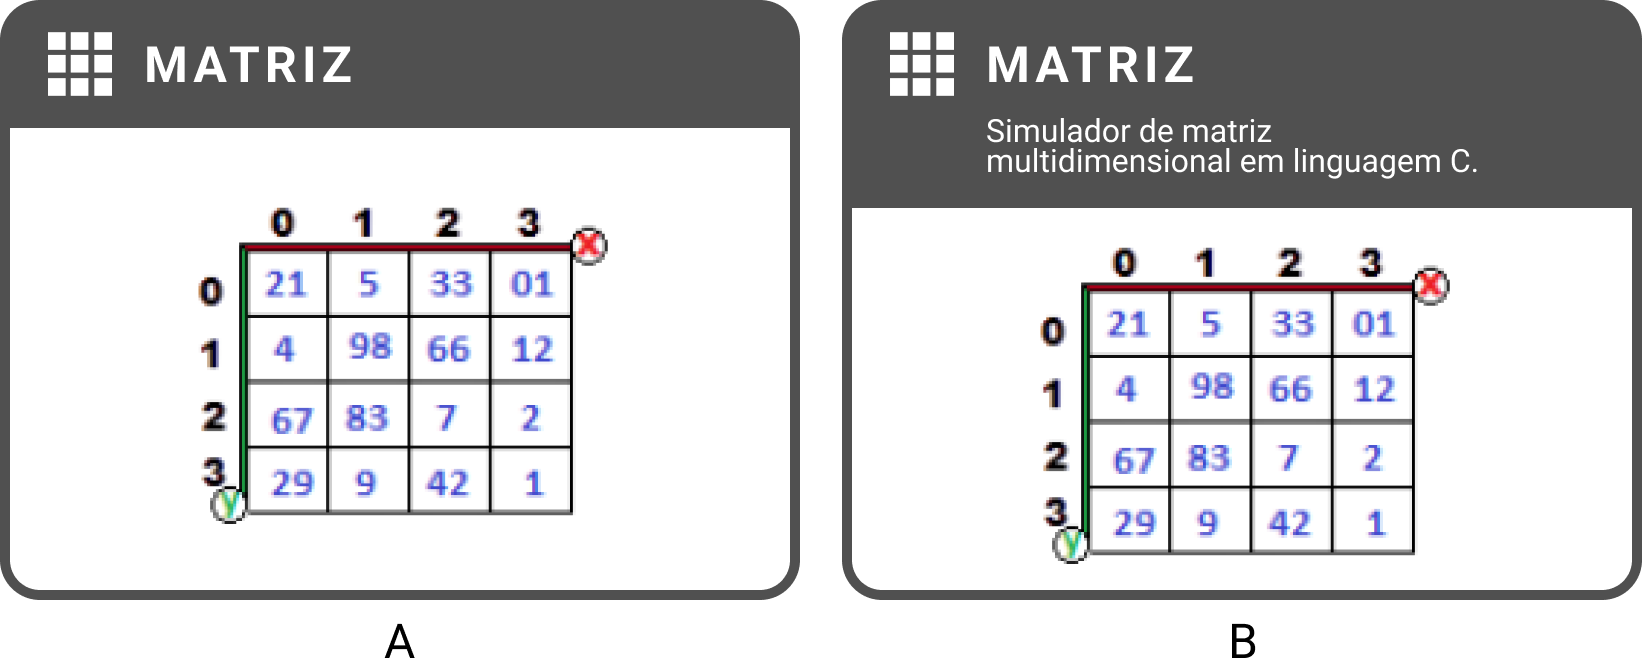
\includegraphics[scale=0.52]{figs/debugandoED-bloco-depois.png}
	\end{center}
        \caption{\label{debugandoED-bloco-depois}Blocos de Matriz (Proposta): (A) sem sobreposição - (B) com sobreposição.}
\end{figure}

Na \autoref{debugandoED-bloco-antes} (A) é apenas uma imagem técnica sobre o bloco, mas como apontando no inicio desta seção, formas mais leigas de identificação são necessárias, não mudando nada para os usuários mais experientes, como na \autoref{debugandoED-bloco-depois} (A), é adicionado o título e o mesmo ícone representativo do menu de navegação, embora não seja obrigatória, proporciona maior acessibilidade e familiaridade aos usuários. 

Na \autoref{debugandoED-bloco-antes} (B), tem-se o efeito de sobreposição do mouse, aqui se repete um desacordo de contraste na utilização das cores e oposição a regra de Flexibilidade e Eficiência da \autoref{Heurísticas de Jakob Nielsen}, no qual o usuário teria de sobrepor o mouse no bloco para assim poder clicar no botão e navegar até a página. Na \autoref{debugandoED-bloco-depois} (B) este botão é removido passando este evento de clique para o bloco em si, não tornando a navegação específica a um botão interno, sendo também mantido o efeito de sobreposição do mouse onde apenas é mostrado uma descrição sobre o conteúdo em si.

Resolvendo também a questão do contraste com a descrição, onde pode ser utilizado uma tonalidade mais escura do próprio bloco e não outra cor, com a fonte na cor branca, criando um contraste nítido e colocando o bloco em cores monocromáticas. As cores em si não são o foco mas sim a disposição do elementos de acordo com a Gestalt, porém tal estudo de cores é de extrema importância para quando se possui um identidade visual definida.

De acordo com o Princípio da Figura-Fundo, para manter o foco nos blocos, cantos arredondados e um contorno, além de estético também servem para fazer embalagens de conteúdo (\autoref{debugandoED-bloco-antes-depois-01} B), isto porque os cantos arredondados estão apontados para a parte interna em direção ao centro do retângulo, desta forma é fácil ver a que lado pertence o retângulo quando estão próximos uns dos outros, diferenciando da \autoref{debugandoED-bloco-antes-depois-01} (A) onde os cantos são poucos arredondados, apresentando um aspecto mais quadrado e agressivo.

O mesmo pode ser notado na \autoref{debugandoED-bloco-antes-depois-01} (B) uma estética minimalista e limpa de acordo com a \autoref{Heurísticas de Jakob Nielsen}, com blocos simples e objetivos, com titulo em ponto focal e imagem em fundo claro.

\begin{figure}[htb]
    \begin{center}
	    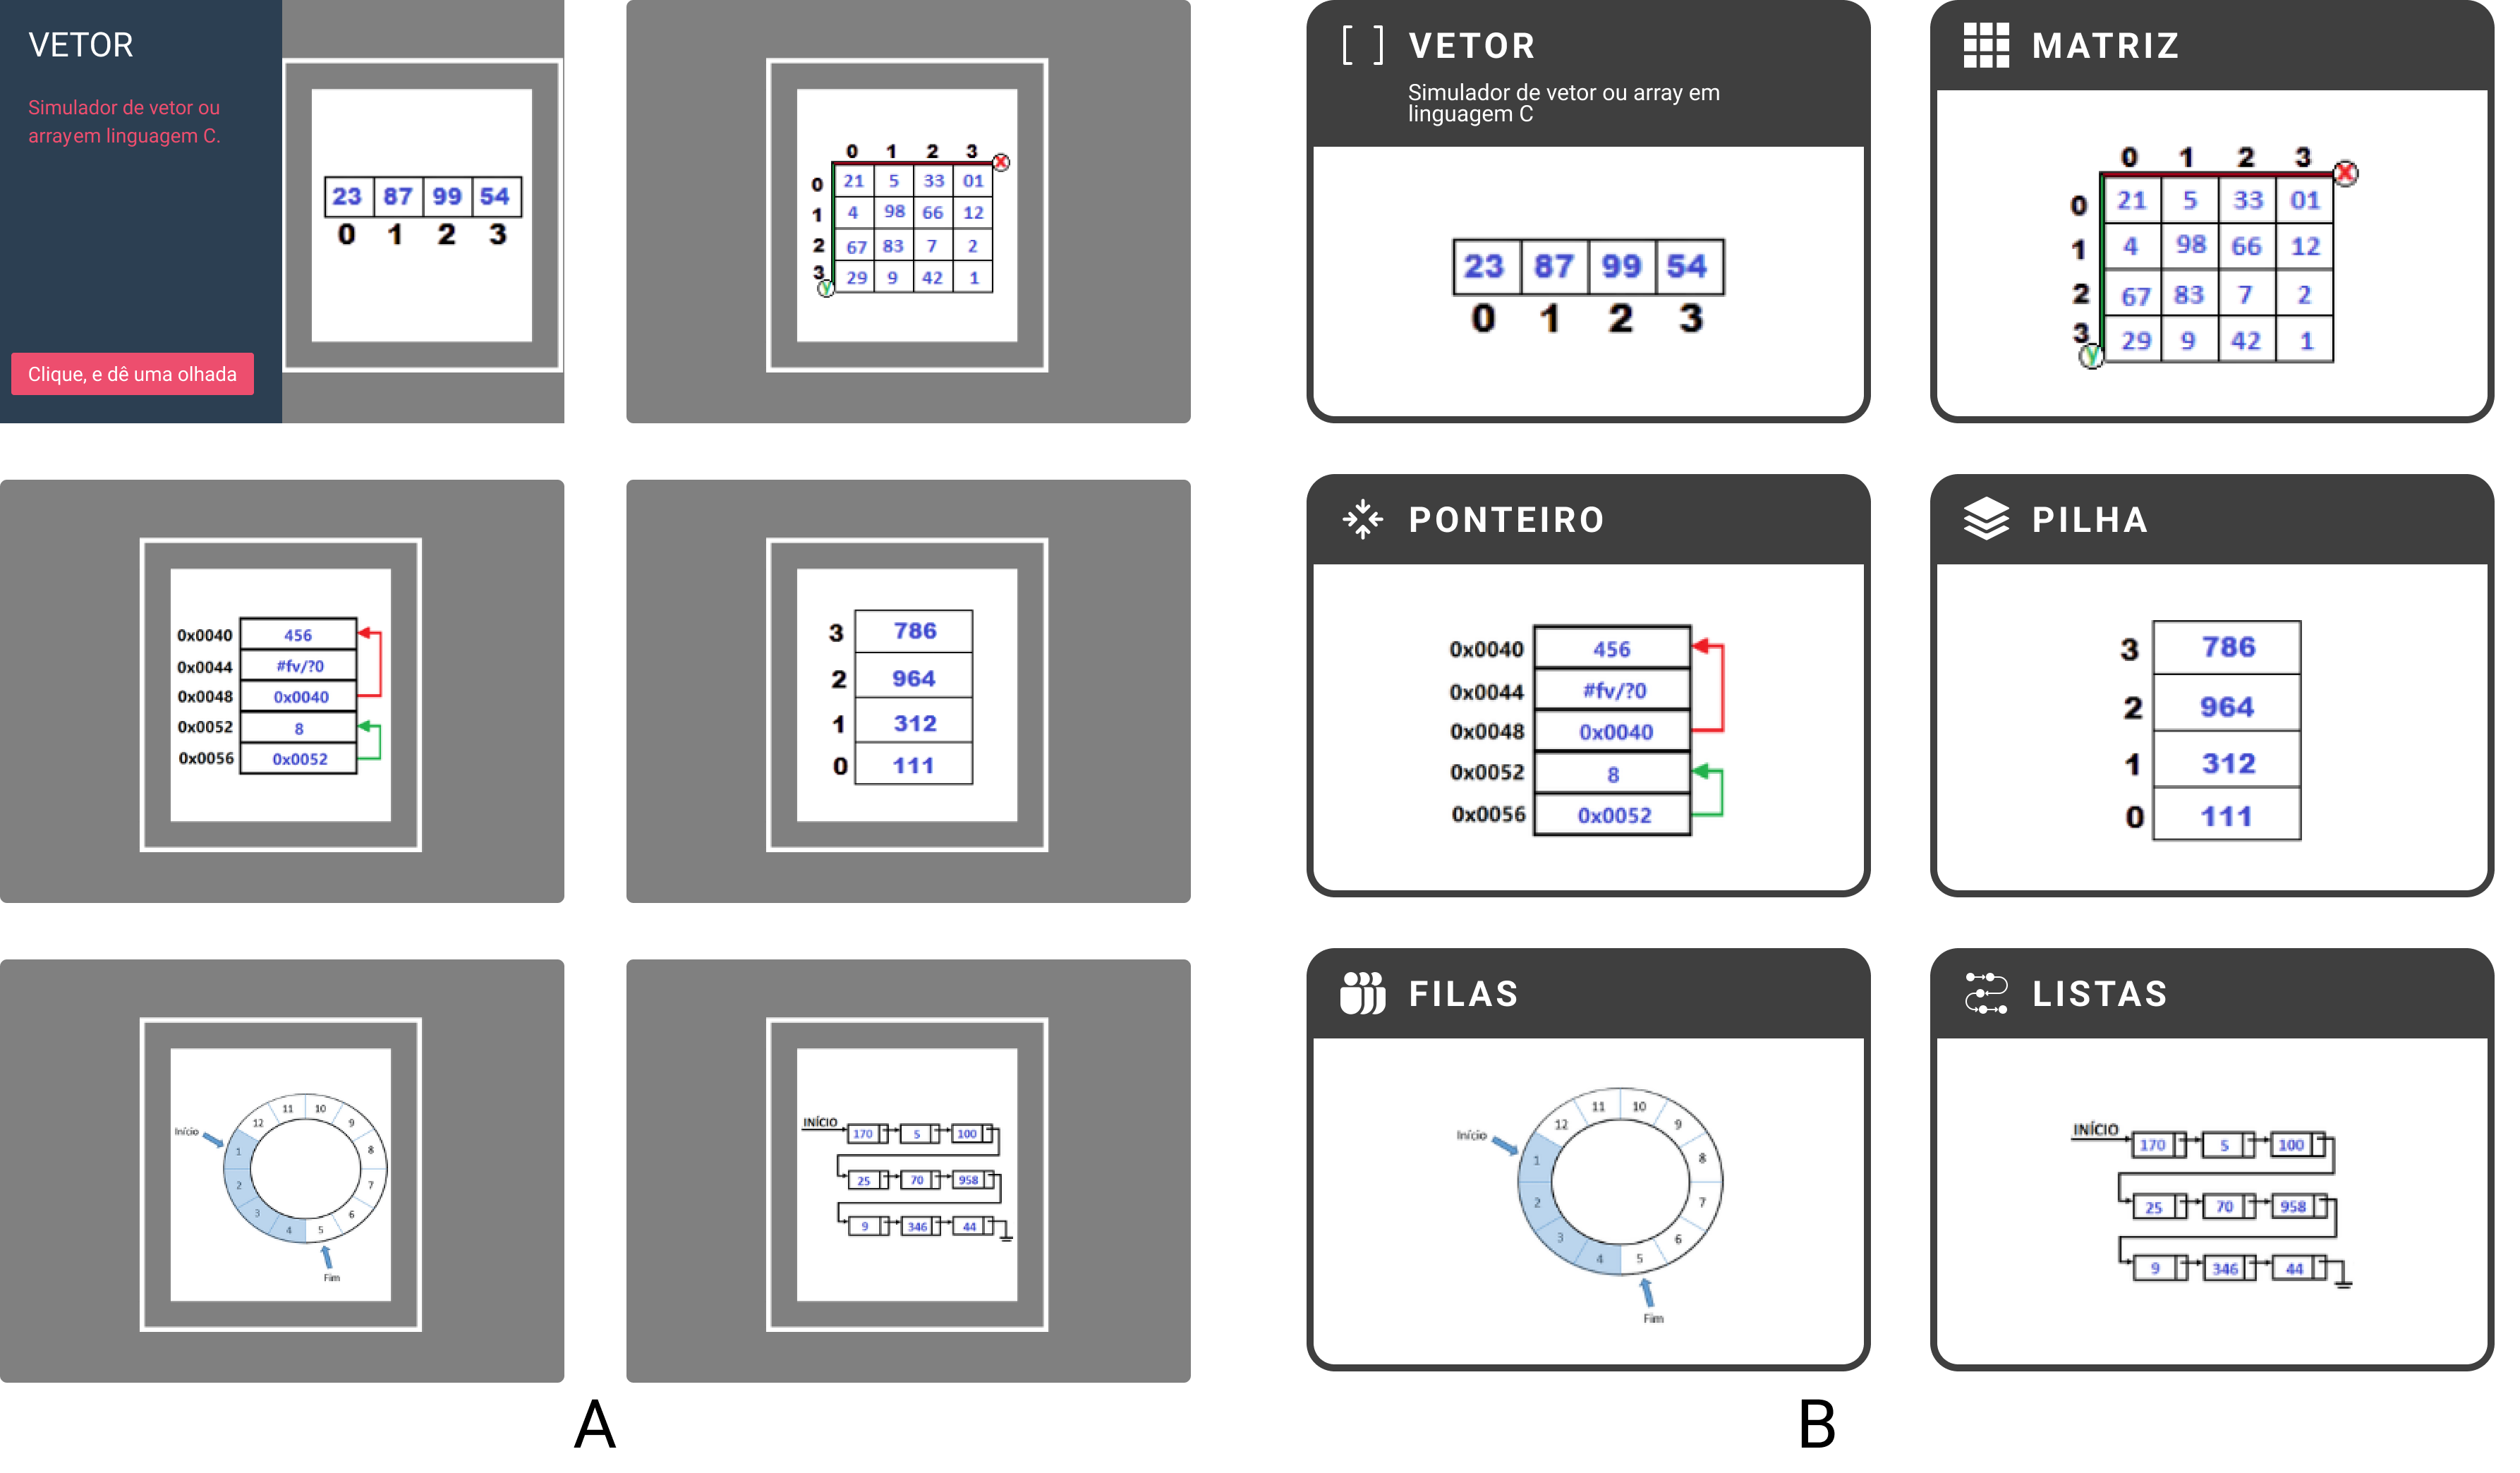
\includegraphics[scale=0.25]{figs/debugandoED-bloco-antes-depois-01.png}
	\end{center}
    \caption{\label{debugandoED-bloco-antes-depois-01}Exemplificação de Todos os Blocos: (A) Original; (B) Proposta.}
\end{figure}

%\newpage

\subsection{Campos de Entrada de Dados}
\label{Campos_de_Entrada_de_Dados}

Na \autoref{debugandoED-inputs}, pode-se notar que o sistema possui dois estilos diferentes de entrada de dados, logo não possui uma padronização nos \textit{inputs}.

Observando com mais cuidado, pode-se notar que várias heurísticas da \autoref{Heurísticas de Jakob Nielsen} são descumpridas, como: Consistência e padrões, nem todos campos possuem “\textit{labels}”; Prevenção de erros, nem todos campos possuem “\textit{tooltip}” indicando erros; Estética e Design minimalista e Auxiliar usuários a reconhecer, campos com variados tamanhos; diagnosticar e recuperar erros, informar melhor ao usuário o erro; e no princípio da Proximidade da \autoref{Princípios de Gestalt}, utilizar do espaçamento para melhor entendimento.

\begin{figure}[ht]
    \begin{center}
	    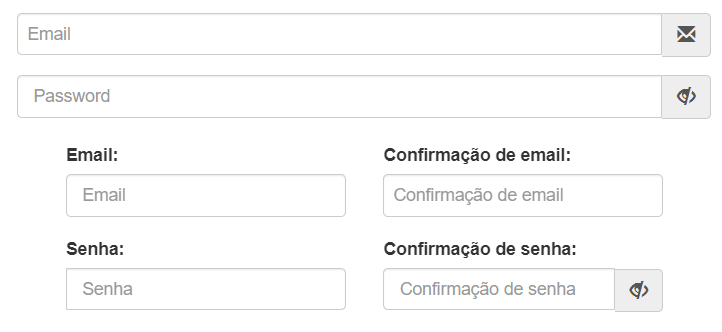
\includegraphics[scale=0.55]{figs/debugandoED-inputs.png}
	\end{center}
    \caption{\label{debugandoED-inputs}Campos de entrada atualmente na Plataforma.}
\end{figure}


Uma forma de resolver tais problemas, é na construção da identidade visual própria para os campos de entrada de dados, comumente os designers utilizam padrões e diretrizes já muito bem estabelecidos neste ramo, em suma a proposta aqui é basear-se na \autoref{Material_Design} que se trata do \textit{Material Design} (\autoref{debugandoED-inputs-md}).

\begin{figure}[ht]
    \begin{center}
	    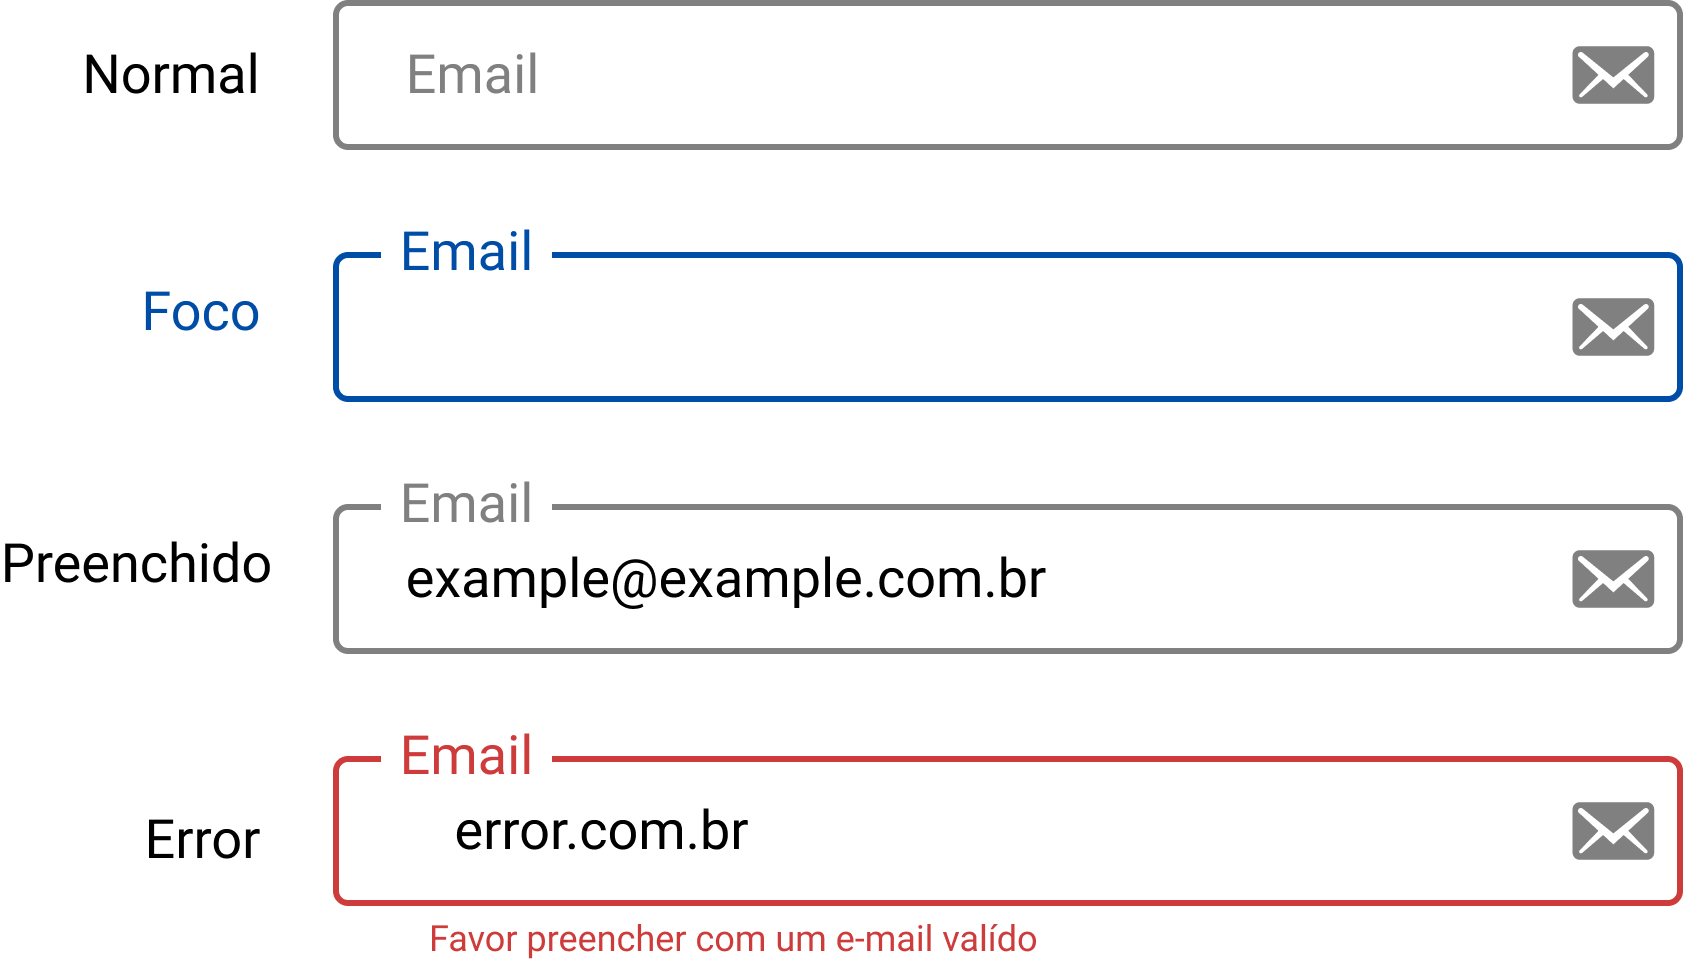
\includegraphics[scale=0.52]{figs/debugandoED-inputs-md.png}
	\end{center}
    \caption{\label{debugandoED-inputs-md}Exemplos de Campos de entrada - Baseados no \textit{Material Design}.}
\end{figure}

Pontos como Prevenção de erros e Auxiliar usuários a reconhecer, diagnosticar e recuperar erros, são muito bem tratados como é o exemplo \textbf{\textit{Error}} na \autoref{debugandoED-inputs-md}, como uma mudança visual na cor do \textit{input} e \textit{label}, como também uma mensagem auxiliando o usuário na correção do erro.

E os outros pontos citados no início desta seção, são resolvidos com a simplicidade e minimalismo no design empregado nestes campos, como o \textit{placeholder} simples. Este, que exibe o tipo do campo,  além do título para orientar o usuário durante o preenchimento.

\subsection{Formulário de Cadastro}
\label{Formulário de Cadastro}

Pensando-se na experiência do usuário, obviamente deve-se realizar uma pesquisa antes de qualquer tomada de decisão, mas pode-se notar na \autoref{debugandoED-form-antes-depois} - Antes, alguns pontos como: o campo de \texttt{Confirmação de email} e a seleção de \texttt{imagem para o perfil} aparentam ser desnecessários, a confirmação do endereço eletrônico pode ser verificada com o envio de um email solicitando uma verificação onde também aumenta a segurança garantindo que aquele endereço eletrônico utilizado no momento do cadastro é de fato do usuário, e a imagem para perfil é algo completamente desnecessário nesse momento, pois tal opção já existe na edição do perfil, sendo assim o formulário fica mais limpo.

Outro ponto relevante a ser considerado é o campo de \texttt{Instituição de ensino}, que atualmente é um \textit{input} do tipo seleção. Contudo, ao analisar a quantidade considerável de opções disponíveis, percebe-se que essa abordagem pode deixar alguns usuários um pouco perdidos. Na minha opinião, uma maneira eficaz de aprimorar esse campo seria permitir a inserção direta e a filtragem entre as opções, o que, sem dúvida, traria uma significativa melhoria na experiência do usuário. Essa melhoria seria ainda mais impactante se fosse implementado um recurso de auto completar, tornando a interação ainda mais intuitiva e eficiente.

O método citado acima pode ser utilizado em demais campos de seleção, como também transformar os campos de \texttt{Estado} e \texttt{Cidade} para seleção utilizando a \ac{API} de  localidades\footnote{\url{https://servicodados.ibge.gov.br/api/docs/localidades}} do IBGE disponibilizada gratuitamente pra propósitos de se obter estados e cidades filtrados.

Devido aos princípios da Continuidade e do Ponto Focal da \autoref{Princípios de Gestalt}, nota-se a inversão dos botões e na suas respectivas estilizações na \autoref{debugandoED-form-antes-depois} (Depois), aumentando o foco e relevância no botão visualmente mais a direita cujo tem maior importância.

A demonstração dos pontos citados anteriormente pode ser visualizados na \autoref{debugandoED-form-antes-depois} (Proposta).

\begin{figure}[htb]
    \begin{center}
	    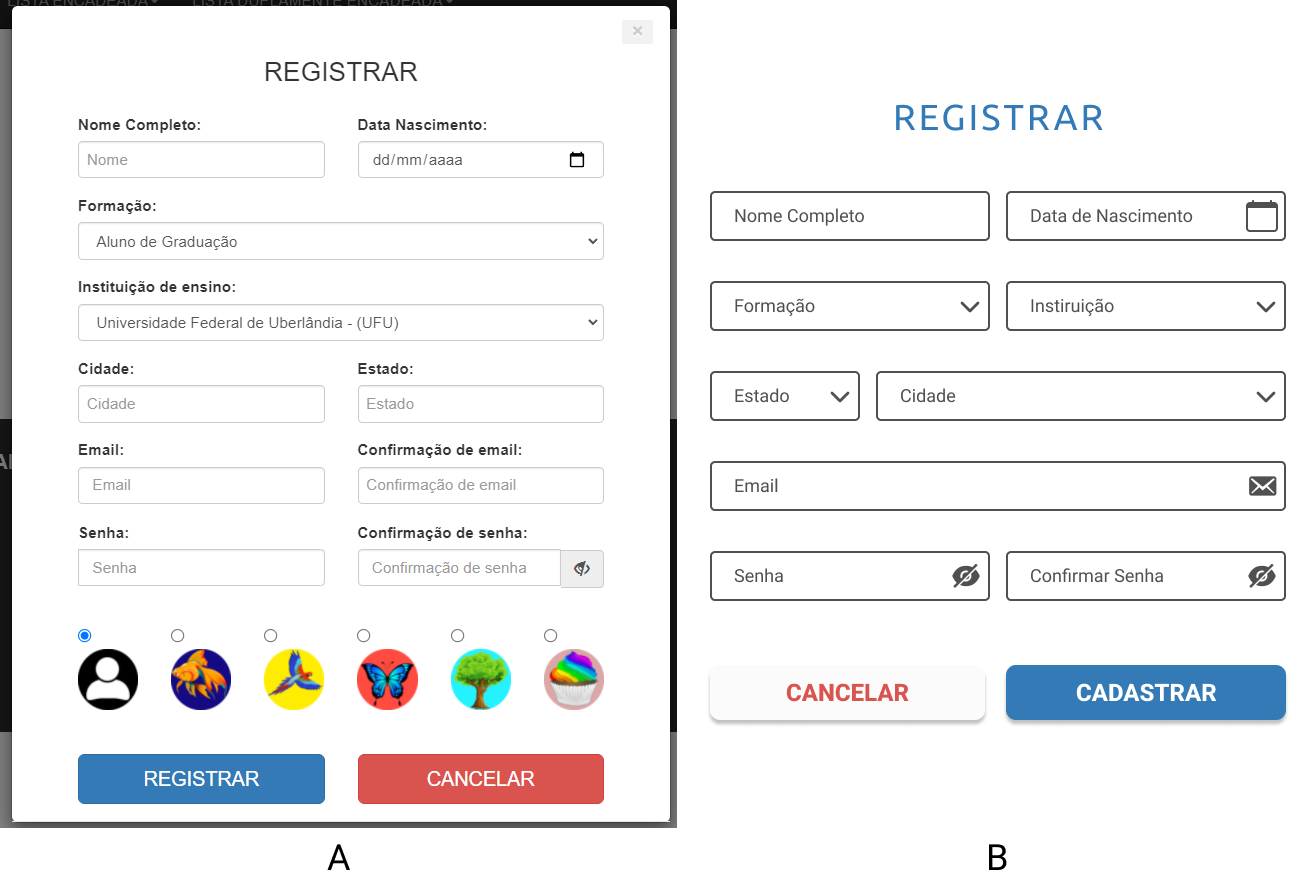
\includegraphics[scale=0.35]{figs/debugandoED-form-antes-depois.png}
	\end{center}
    \caption{\label{debugandoED-form-antes-depois}Formulário de Cadastro: (A) Original; (B) Proposta.}
\end{figure}

\subsection{Formulário de Login}
\label{Formulário de Login}
Como discutido na \autoref{Formulário de Cadastro}, os princípios da Continuidade e do Ponto Focal mantêm sua relevância na \autoref{debugandoED-form-login-antes-depois}. Neste contexto, destaco a presença de dois botões, sendo que o local do botão mais à direita não possui uma importância destacada neste fluxo específico. Para contornar essa situação, optou-se por remover o botão de cadastro, substituindo-o de maneira sucinta por um link posicionado logo abaixo do botão “\texttt{Entrar}”.

Outro ponto que merece atenção, e isso se refere ao princípio da Região Comum, conforme apresentado na \autoref{Princípios de Gestalt}. A solução para esse aspecto é relativamente simples, pois a aplicação de espaçamentos adequados ou até mesmo a remoção das linhas horizontais já seria o suficiente para proporcionar o espaçamento necessário e melhorar a organização visual do layout.

\begin{figure}[htb]
    \begin{center}
	    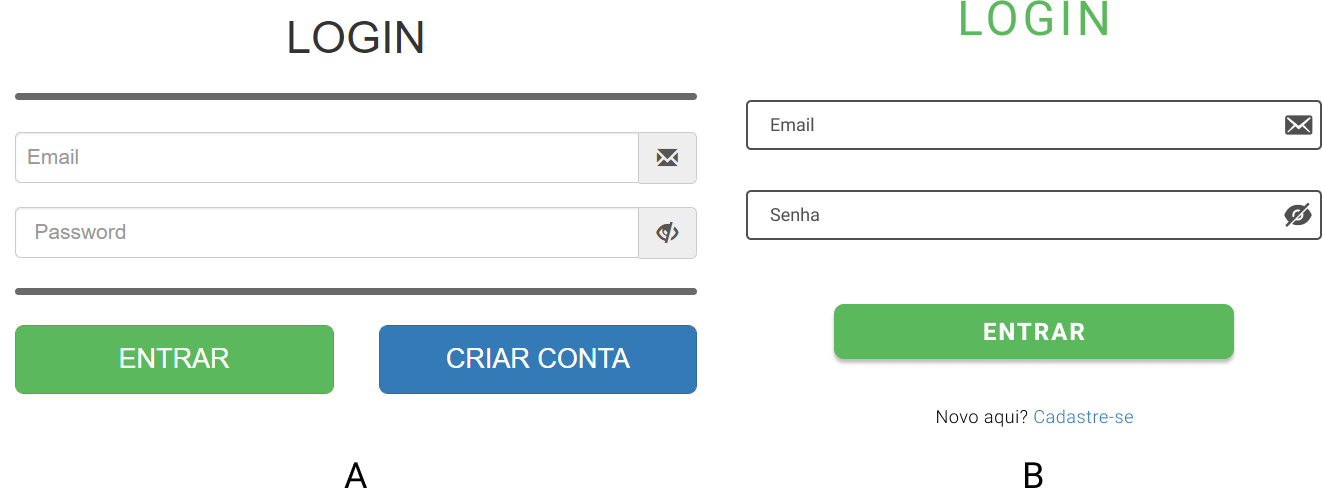
\includegraphics[scale=0.35]{figs/debugandoED-form-login-antes-depois.png}
	\end{center}
    \caption{\label{debugandoED-form-login-antes-depois}Formulário de Login: (A) Original; (B) Proposta.}
\end{figure}

\subsection{Conteúdo das Telas de Simulação}
\label{Conteúdo das Telas de Simulação}

As Figuras \ref{debugandoED-ponteiro-antes-01} e \ref{debugandoED-ponteiro-antes-02} são, respectivamente, capturas de tela do início e durante a simulação referente à execução de um ponteiro no contexto de programação.

\begin{figure}[htb]
    \begin{center}
	    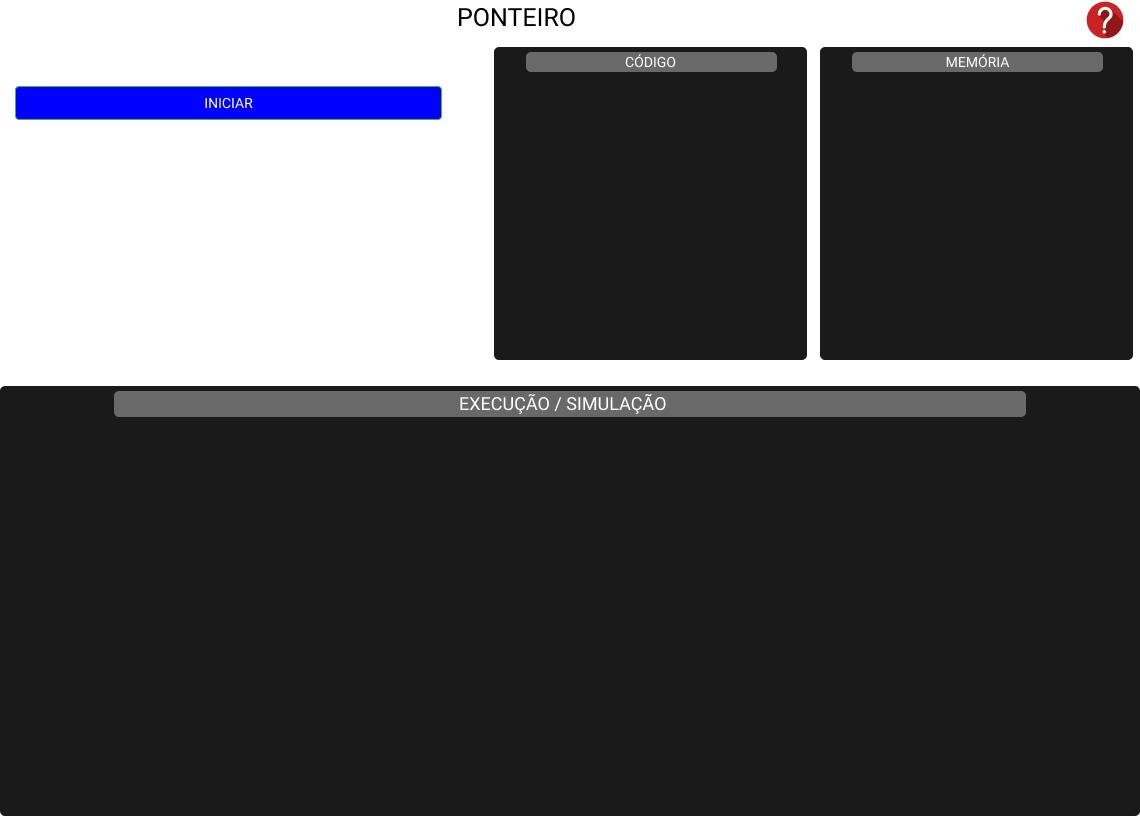
\includegraphics[scale=0.25]{figs/debugandoED-ponteiro-antes-01.png}
	\end{center}
    \caption{\label{debugandoED-ponteiro-antes-01}Simulação de Ponteiro - 1º Momento}
\end{figure}

Inicialmente na \autoref{debugandoED-ponteiro-antes-01}, nota-se apenas os quadros em fundo escuro, o que necessariamente não é um problema, mas sim uma identidade visual dependendo da comunicabilidade cujo desenvolvedor quer passar ao usuário final, porém, tais quadros também podem ser dispostos em uma tonalidade mais clara, obtendo um visual mais limpo com contraste não tão agressivos.

\begin{figure}[htb]
    \begin{center}
	    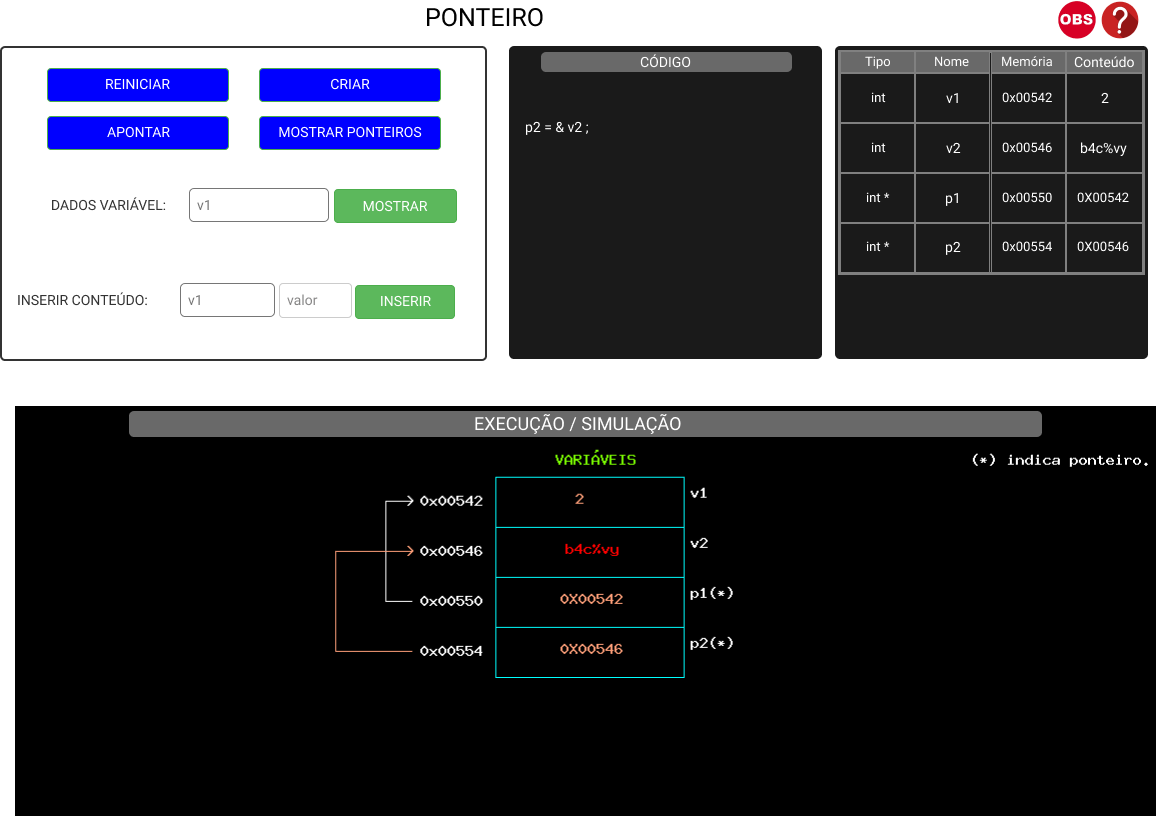
\includegraphics[scale=0.25]{figs/debugandoED-ponteiro-antes-02.png}
	\end{center}
    \caption{\label{debugandoED-ponteiro-antes-02}Simulação de Ponteiro - 2º Momento}
\end{figure}

\begin{figure}[htb]
    \begin{center}
	    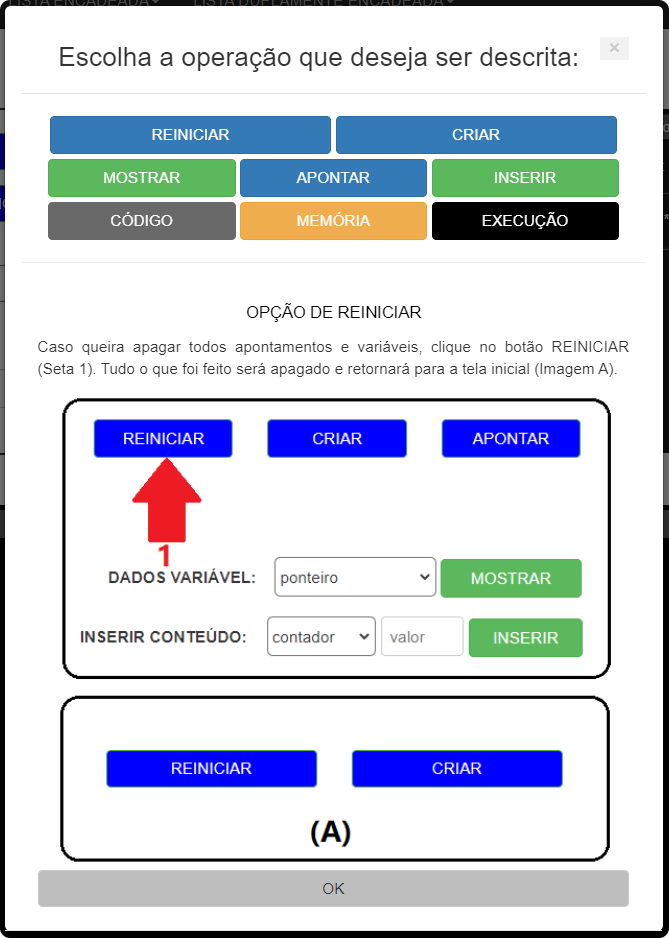
\includegraphics[scale=0.25]{figs/debugandoED-modais-help-01.png}
	\end{center}
    \caption{\label{debugandoED-modais-help-01}Modal de ajuda envolvidos na simulação de ponteiro}
\end{figure}

\begin{figure}[htb]
    \begin{center}
	    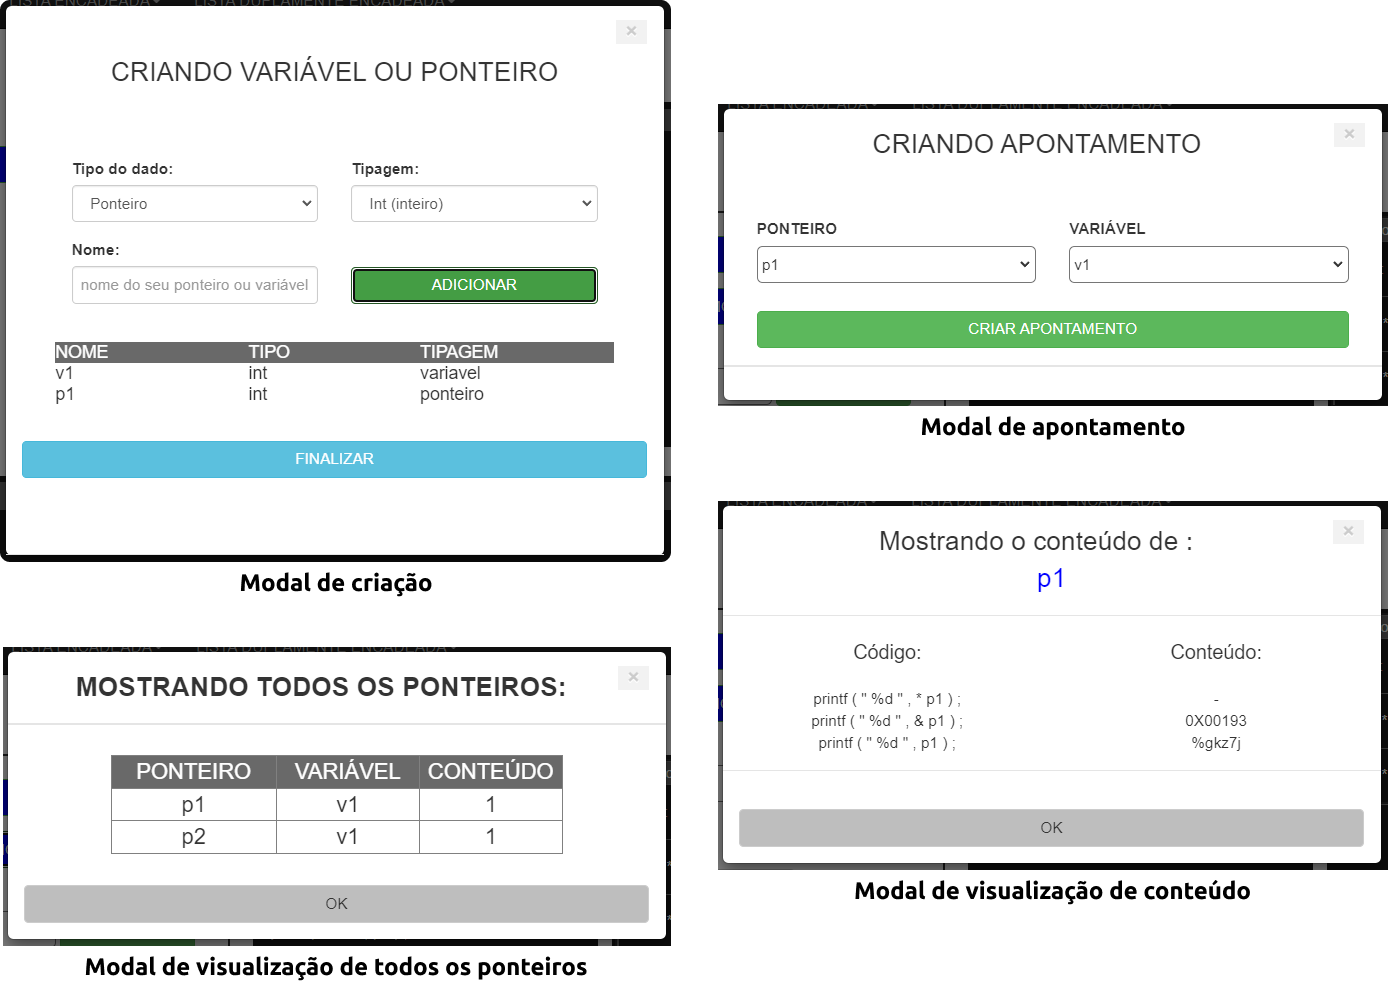
\includegraphics[scale=0.25]{figs/debugandoED-modais-antes-01.png}
	\end{center}
    \caption{\label{debugandoED-modais-antes-01}Modais envolvidos na simulação de ponteiro}
\end{figure}

A \autoref{debugandoED-ponteiro-antes-02}, nota-se que os quadros negros estão preenchidos com seus devidos conteúdos didáticos referente a uma simulação de ponteiro no contexto de programação, no mesmo pode-se notar, que o botão “\texttt{Iniciar}” deu lugar a um quadro com mais informações e ações para progredir na simulação, porém, de acordo com \autoref{Heurísticas de Jakob Nielsen}, algumas heurísticas não são totalmente exploradas corretamente, como:
\begin{itemize}
    \item A liberdade e controle do usuário, devido ao usuário ter que necessariamente realizar as ações da simulação através de modal (\autoref{debugandoED-modais-antes-01}) e devido a isso, caso precise consultar a documentação deverá fechar o modal e recomeçar.
    
    Pode-se observar na \autoref{debugandoED-modais-antes-01}, a falta consistência e padrões, como títulos em caixa alta e caixa baixa, em negrito e normal e falta de alinhamento em alguns elementos

    \item Reconhecer ao invés de lembrar é pouca explorada, pois, os botões possuem o mesmo padrão de cores, porém, com funções distintas, o que pode causar confusão no usuário na hora da utilização.

    \item Ajuda e documentação, até possui um modal dedicado a tais explicações para que o usuário não se percam na simulação. Porém, é muito densa a quantidade de informação em apenas um único local, outro ponto, é a falta de padronização nas cores dos botões dentro do modal como é mostrado na \autoref{debugandoED-modais-help-01} em relação aos botões reais no sistema.

\end{itemize}

As melhorias projetadas nas Figuras \ref{debugandoED-ponteiro-depois-01} e \ref{debugandoED-ponteiro-depois-02}, demonstra uma percepção no questionário realizado em termos de usabilidade e \ac{UX}. Obtendo uma evolução na comunicabilidade do simulador. O design da interface \ac{UI} foi refinado para promover uma interação mais intuitiva, alinhando-se com os princípios da \autoref{Princípios de Gestalt} para facilitar o reconhecimento de padrões.

\begin{figure}[htb]
    \begin{center}
        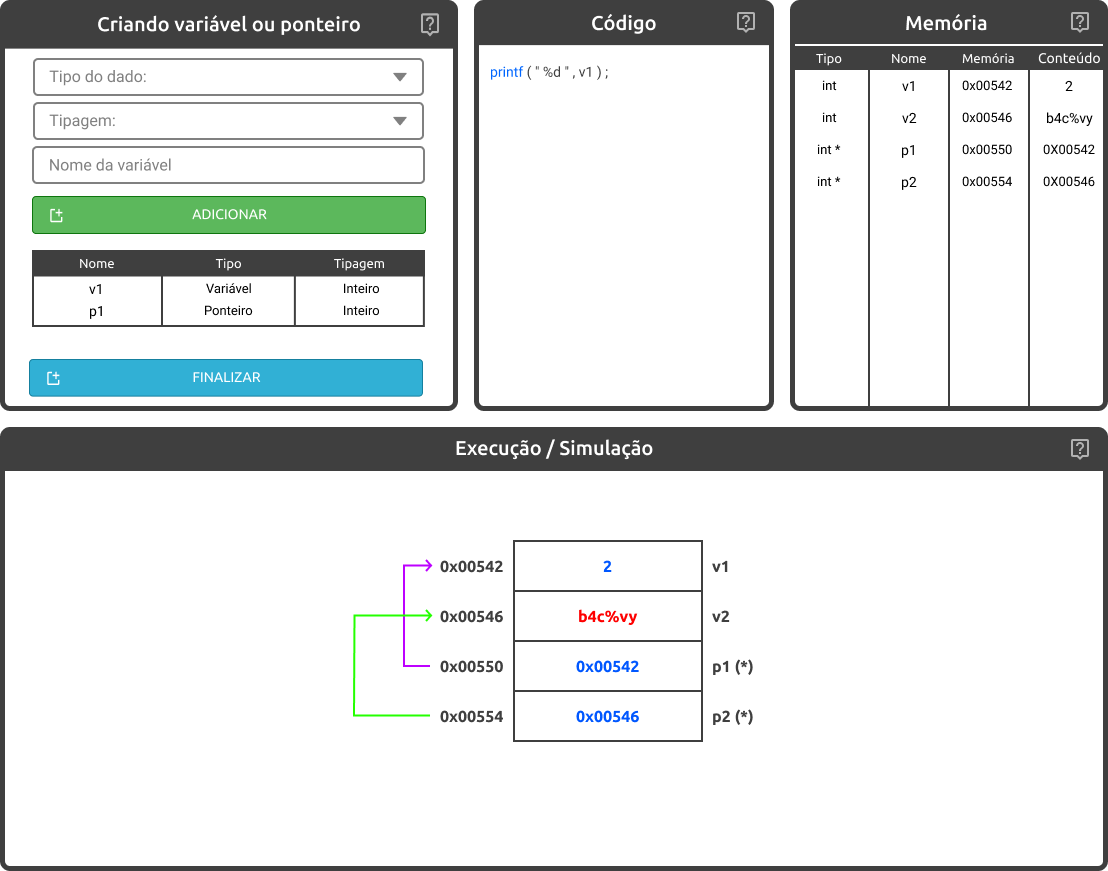
\includegraphics[scale=0.25]{figs/debugandoED-ponteiro-depois-01.png}
    \end{center}
    \caption{\label{debugandoED-ponteiro-depois-01}Simulação de Ponteiro - Melhorias Projetadas 1}
\end{figure}

\begin{figure}[htb]
    \begin{center}
        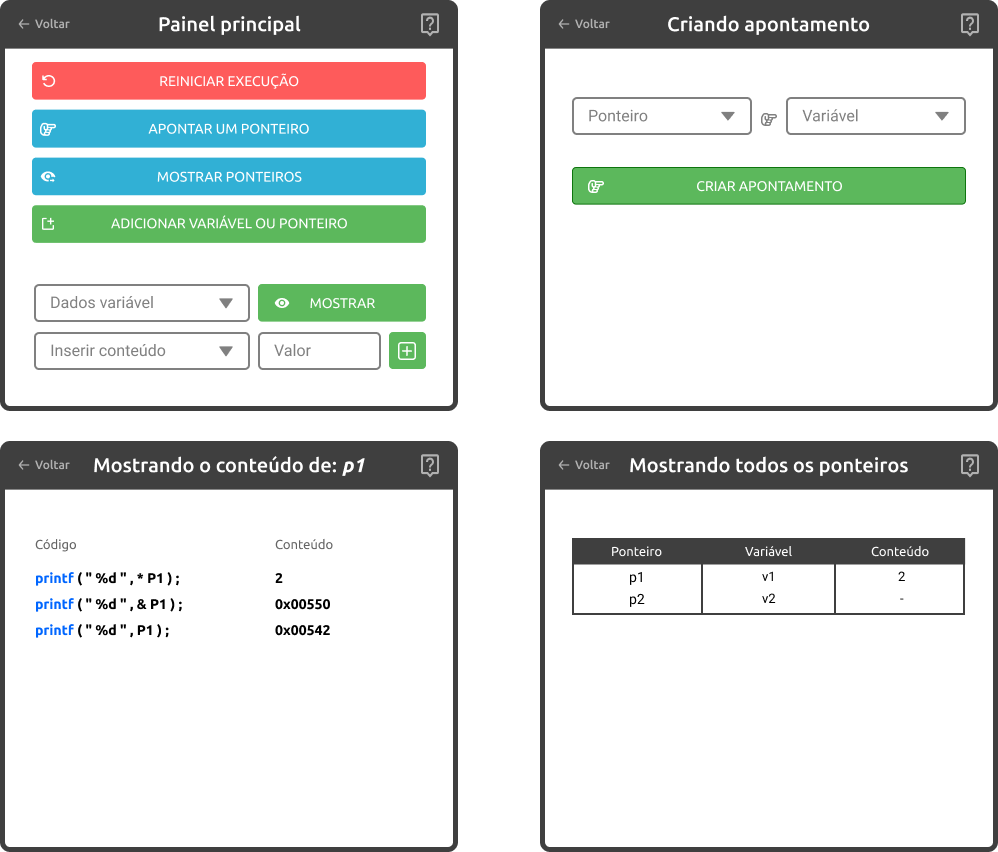
\includegraphics[scale=0.25]{figs/debugandoED-ponteiro-depois-02.png}
    \end{center}
    \caption{\label{debugandoED-ponteiro-depois-02}Simulação de Ponteiro - Melhorias Projetadas 2}
\end{figure}

Apresentando uma \ac{UI} aprimorada, com a utilização de esquemas de cores e tipografia para melhorar a legibilidade e a hierarquia visual, seguindo os princípios da \autoref{Princípios de Gestalt} para agrupamento e alinhamento. O design limpo e intuitivo promove uma experiência de usuário \ac{UX} positiva, em conformidade com as heurísticas de usabilidade da \autoref{Heurísticas de Jakob Nielsen}, particularmente no que diz respeito à consistência e padronização dos elementos de \ac{UI}.

A estrutura da informação e os elementos de navegação foram reorganizados para dar ao usuário maior controle e liberdade, permitindo uma exploração mais fluída e natural. Isso é evidente na inclusão de \textit{tooltips} e modais informativos, que são facilmente acessíveis sem interromper a tarefa do usuário, alinhando-se com o princípio de Ajuda e documentação das heurísticas de Nielsen.

Essas melhorias de interface não apenas aprimoram a estética, mas também reforçam a funcionalidade e a eficácia pedagógica da simulação, ao passo que a experiência de aprendizado se torna mais engajante e menos suscetível a erros de interpretação ou operação

\section{Análise das Propostas por Experimento}
\label{secAnálisePropostasExperimento}

Esta seção apresentará as respostas obtidas nos questionários da pesquisa conduzida para este estudo. O objetivo principal é fornecer uma visão abrangente das percepções e opiniões coletadas por duas abordagens distintas: em relação à usabilidade e design e a experiência do usuário em interfaces da plataforma. As diferenças demográficas e de formação educacional entre esses dois grupos proporcionaram uma visão diversificada e enriquecedora das opiniões e perspectivas dos usuários. Foram conduzidos 2 experimentos: um voltado para estudantes e outro focado em profissionais. 

Para a realização dos experimentos, foram criados dois questionários para coletar dados sobre as percepções dos participantes em relação a plataforma \href{https://debugandoed.facom.ufu.br/}{DebugandoED} e suas respectivas telas propostas neste trabalho. Ambos os questionários compartilharam uma série de perguntas idênticas, com o propósito de avaliar as telas de login, cadastro, tela principal e tela de conteúdo. A distinção crítica entre os questionários ocorreu na primeira parte, na qual as perguntas demográficas e de conhecimento foram apresentadas aos participantes. Dentre as diversas questões, algumas delas baseiam-se na escolha entre telas (\autoref{fomuEscolha}), possibilitando a escolha da ``Imagem A'' (tela original da plataforma) ou ``Imagem B'' (proposta da mesma tela utilizando os conceitos/princípios).

\begin{figure}[ht]
    \begin{center}
	    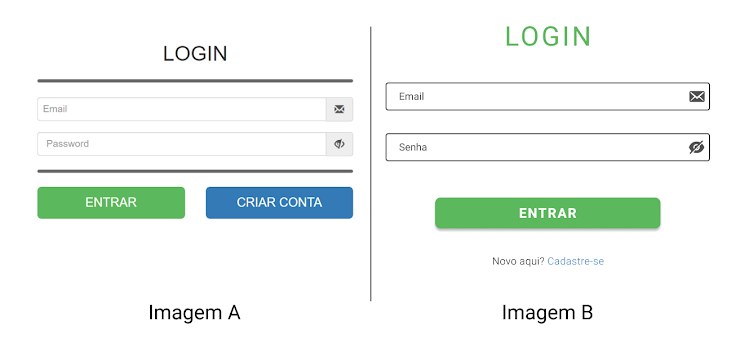
\includegraphics[scale=0.4]{figs/form_compara.png}
	\end{center}
    \caption{\label{fomuEscolha}Exemplo das imagens utilizadas nos questionários.}
\end{figure}

Todos os detalhes sobre os questionários, bem como todas as questões utilizadas, estão no \autoref{questionario_de_pesquisa}.

\subsection{Pesquisa de Opinião com Estudantes}
\label{Pesquisa_de_Opinião_com_Estudantes}

A pesquisa contou com a participação de um grupo diversificado de 33 respondentes, incluindo indivíduos de diferentes gêneros, faixas etárias, níveis de escolaridade e profissões (Figuras \ref{APB_01} e \ref{APB_02}). Os participantes variaram desde estudantes do ensino médio até aqueles com pós-doutorado e experiência em áreas como tecnologia, atendimento ao cliente, e ciências biológicas. Além disso, houve uma distribuição de níveis de experiência, com participantes desde juniores até sêniores em suas carreiras.

Para garantir a integridade ética da coleta de percepções, foram adotadas medidas cuidadosas. Preocupações éticas relacionadas à privacidade e confidencialidade foram consideradas durante a coleta. Os questionários foram elaborados de forma anônima, dispensando a identificação dos participantes, o que assegura a proteção dos dados coletados. Adicionalmente, foi solicitado o consentimento informado dos participantes antes da aplicação dos questionários. Esse processo esclareceu os objetivos da pesquisa, garantindo a livre escolha de participação e reforçando a importância da proteção dos dados.

Além de suas características demográficas e educacionais, os participantes também foram questionados sobre seu conhecimento em \ac{UI} e \ac{UX} (\autoref{APB_03}), com algumas pessoas afirmando ter um entendimento desses conceitos, enquanto outras não estavam familiarizadas. No que diz respeito à \ac{UI}, 18 participantes afirmaram ter conhecimento, enquanto 15 declararam não estar familiarizados. Quanto à \ac{UX}, 13 participantes afirmaram ter conhecimento, enquanto 20 indicaram não estar familiarizados com o termo.

Esta diversidade de perfil dos participantes enriqueceu a pesquisa, fornecendo uma variedade de perspectivas e experiências que contribuíram para uma análise abrangente das telas de interface do usuário e da experiência do usuário. 

Além disso, é importante destacar que o \autoref{respostas_dos_estudantes} contém capturas de tela detalhadas exclusivamente das respostas do grupo de estudantes, proporcionando uma visão mais aprofundada das percepções dessa parcela específica de participantes na pesquisa.

Após a análise e avaliação das respostas dos participantes, tem-se: 

\begin{itemize}
    \item \textbf{Análise das Telas de Login}
    
    Durante esta pesquisa, foram avaliadas as telas de login em vários aspectos de usabilidade e design. Os resultados revelaram uma clara preferência pela ``Imagem B'' em categorias cruciais, como \textit{layout} atrativo, experiência intuitiva, organização de informações clara e distribuição eficiente de campos de entrada. No entanto, a ``Imagem A'' recebeu elogios por sua mensagem de erro e rótulos de botões informativos. Alguns participantes sugeriram combinar as duas telas, destacando pontos fortes de cada uma. Em resumo, enquanto a ``Imagem B'' se destacou como a escolha preferida na maioria das categorias, a ``Imagem A'' demonstrou pontos fortes específicos que merecem consideração na otimização da experiência do usuário.
    
    \item \textbf{Análise das Telas de Cadastro}
    
    Na análise comparativa para a tela de cadastro, observou-se uma preferência geral pelos elementos da ``Imagem B'' em diversas categorias, incluindo \textit{layout}, organização, distribuição de campos de entrada, mensagens de erro e conteúdo textual. A ``Imagem A'' recebeu elogios por sua estética visual, enquanto a ``Imagem B'' se destacou por oferecer uma experiência mais intuitiva e funcional. As sugestões apontaram para a possibilidade de combinar as forças de ambas as imagens, aproveitando a estética da ``Imagem A'' com a funcionalidade da ``Imagem B'', ressaltando a importância de equilibrar forma e função na criação de interfaces de usuário.
    
    \item \textbf{Análise da Tela Principal}
    
    Na avaliação para a tela principal, a preferência geral recai sobre a ``Imagem B'' em uma série de aspectos, incluindo o \textit{layout} atrativo, abordagem objetiva na disposição de elementos, experiência de uso confortável, organização eficiente de informações, distribuição equilibrada de elementos e clareza nos blocos de conteúdo. A ``Imagem A'' foi elogiada apenas por sua estética visual em algumas respostas. A sugestão apontada é a de que a ``Imagem B'' poderia ser aprimorada com cores mais claras nos elementos do corpo da página, semelhantes à ``Imagem A''. A predominância da preferência pela ``Imagem B'' sugere uma abordagem mais funcional e eficaz na criação da tela principal.
    
    \item \textbf{Análise da Tela de Conteúdo}
    
    Na avaliação para a tela de conteúdo, a preferência geral recai sobre a ``Imagem B'' em diversos aspectos, incluindo o layout atrativo, abordagem objetiva na disposição e organização dos blocos de conteúdo, experiência de uso confortável, organização eficiente de informações e distribuição equilibrada de elementos. A sugestão apontada é a de que a ``Imagem B'' poderia incorporar um modo escuro (\textit{dark mode}) para maior conforto visual, especialmente ao exibir código na tela. A predominância da preferência pela ``Imagem B'' sugere que sua abordagem é mais eficaz e intuitiva para a apresentação de conteúdo.
\end{itemize}

Em suma, os resultados da análise das telas de login, cadastro, tela principal e tela de conteúdo revelaram uma tendência clara em favor da ``Imagem B'' por parte dos estudantes que participaram do questionário. Essa preferência foi fundamentada em vários aspectos, como \textit{layout} atrativo, organização intuitiva, distribuição eficiente de informações e mensagens de erro adequadas. No entanto, é importante notar que a ``Imagem A'' também recebeu elogios por sua estética visual e pela presença de \textit{labels} no formulário, que foram considerados benéficos para usuários com mais idade.

As sugestões dos participantes apontaram para a possibilidade de combinar elementos positivos de ambas as imagens, destacando a importância de equilibrar forma e função na criação de interfaces de usuário. Além disso, houve recomendações para melhorias específicas, como a incorporação de um modo escuro na ``Imagem B'' para melhorar o conforto visual durante a visualização de código.

Em última análise, os resultados enfatizam a importância de considerar as preferências e necessidades dos usuários ao projetar interfaces, buscando o equilíbrio entre estética e funcionalidade para proporcionar uma experiência de usuário superior.


\vspace{10pt}
\subsection{Pesquisa de Opinião com Profissionais}
\label{Pesquisa_de_Opinião_com_Profissionais}

A pesquisa foi conduzida com um grupo de participantes que demonstram uma forte ligação com o campo do desenvolvimento de software e áreas relacionadas. Estes respondentes apresentam uma variedade de perfis, incluindo diferentes faixas etárias e níveis de escolaridade, com muitos deles possuindo graduações e especializações.

A maioria dos participantes está atualmente trabalhando com desenvolvimento de software ou funções semelhantes, ocupando cargos que variam de estagiários a profissionais sêniores. Suas profissões abrangem várias áreas, como desenvolvedores \textit{full stack}, engenheiros de software, programadores, entre outros. Essa diversidade de cargos e níveis de experiência contribui para uma visão abrangente das perspectivas dos profissionais de desenvolvimento.

Além disso, a pesquisa contou com 11 profissionais, cujas informações demográficas estão detalhadas nas Figuras \ref{APC_01}, \ref{APC_02} e \ref{APC_03}. Destaca-se que apenas 1 participante deste grupo indicou não ter familiaridade com os conceitos de \ac{UI} e \ac{UX}. O conhecimento específico desses profissionais em \ac{UI} e \ac{UX} pode ser encontrado na \autoref{APC_03}. Todas as respostas desse grupo estão compiladas no \autoref{respostas_dos_profissionais}, que consiste em capturas de tela detalhadas das respostas fornecidas por cada profissional participante da pesquisa.

A partir dessas informações, foi possível esperar que as respostas e avaliações dos participantes forneçam \textit{insights} valiosos sobre as telas de interface do usuário e a experiência do usuário, com base em suas experiências e conhecimentos especializados. Essa perspectiva especializada é fundamental para uma análise aprofundada da pesquisa em questão. 

\vspace{10pt}
Após a análise e avaliação das respostas dos participantes, tem-se: 

\begin{itemize}
    \item \textbf{Análise da Tela de Login}
    
    Durante a pesquisa, ao se comparar as duas telas de login, nota-se uma clara preferência pela ``Imagem B'' entre os participantes. Esta foi considerada mais atrativa, intuitiva e com uma organização de informações superior. Além disso, a ``Imagem B'' se destacou por possuir uma distribuição mais eficiente dos campos de entrada e mensagens de erro adequadas. Apesar de algumas críticas pontuais à ``Imagem A'', como a presença de elementos visuais excessivos e possíveis problemas de legibilidade, a maioria dos participantes concordou que a ``Imagem B'' é a opção mais objetiva e eficaz para fazer login.

    \item \textbf{Análise da Tela de Cadastro}
    
    As telas de cadastro também foram avaliadas, e novamente, a ``Imagem B'' se destacou. Esta foi consistentemente elogiada por sua organização, intuitividade e mensagens de erro adequadas. Por outro lado, a ``Imagem A'' muitas vezes foi vista como sobrecarregada de informações ou elementos visuais excessivos. Por outro lado, um ponto positivo da ``Imagem A'' foi a presença de \textit{labels} no formulário, que os participantes consideraram úteis, especialmente para os usuários com mais idade. Portanto, este estudo indica a preferência pela ``Imagem B'' para fins de cadastro, mas também ressalta a importância de considerar características específicas, como os \textit{labels}, para melhorar a experiência do usuário.
    
    \item \textbf{Análise da Tela Principal}
    
    Ao avaliar a tela da página principal, a ``Imagem B'' se destacou em aspectos cruciais, como \textit{layout}, organização e funcionalidade. Esta foi consistentemente escolhida pelos participantes como a mais eficaz em proporcionar uma experiência de usuário intuitiva e visualmente agradável. Embora a ``Imagem A'' tenha recebido algumas críticas, como a presença de informações excessivas, ainda foi elogiada por sua navegação em alguns casos. Em resumo, os resultados indicam uma clara preferência dos participantes pela ``Imagem B'' em design e usabilidade.

    \item \textbf{Análise da Tela de Conteúdo}
    
    Ao analisar as respostas sobre a a tela de conteúdo, percebe-se que a maioria preferiu a ``Imagem B'' em design atrativo, organização, interatividade e consistência textual. A ``Imagem B'' se destacou principalmente por sua abordagem objetiva, distribuição equilibrada de elementos e eficiência na apresentação das informações. Por outro lado, a ``Imagem A'' foi ocasionalmente apontada como tendo excesso de informações ou elementos visuais, o que pode prejudicar a experiência do usuário. Em resumo, a maioria dos participantes identificou a ``Imagem B'' como a opção mais adequada para proporcionar uma experiência de usuário superior na apresentação de conteúdo.
    
\end{itemize}

Em síntese, a análise abrangente das quatro áreas distintas, com base nas respostas de profissionais da área, revelou uma clara preferência pela ``Imagem B'' em quase todos os aspectos avaliados. Essa preferência foi fundamentada na atratividade visual, intuição, organização eficaz de informações e distribuição eficiente de elementos.

Apesar disso, a ``Imagem A'' não deve ser ignorada, pois, demonstrou méritos específicos, como a presença de \textit{labels} úteis para facilitar a experiência de usuários com mais idade. Portanto, a pesquisa indica a ``Imagem B'' como a escolha preferencial para a tela de login, cadastro, tela principal e tela de conteúdo. No entanto, destaca-se a importância de avaliar cuidadosamente as características específicas de cada imagem, aproveitando os pontos fortes de ambas, para otimizar a experiência do usuário de maneira global e eficaz.

	
	% ---
	% Finaliza a parte no bookmark do PDF, para que se inicie o bookmark na raiz
	% ---
	\bookmarksetup{startatroot} 
	% ---
	
	% ---
	% Conclusão
	% ---
	\chapter[Conclusão]{Conclusão}
\label{capConclusao}

Este trabalho teve como principal objetivo aprofundar a compreensão de elementos fundamentais no \textit{design} de interfaces de sistemas, abrangendo temas como usabilidade, comunicabilidade, acessibilidade, experiencia de usuário, interface de usuário e técnicas de avaliação da usabilidade. O estudo iniciou-se com uma revisão teórica aprofundada, onde conceitos propostos por renomados profissionais da área, como Jakob Nielsen, foram discutidos em conjunção com princípios da psicologia da forma, Gestalt, e diretrizes contemporâneas de design, como o Material Design.

A fase empírica do estudo envolveu a aplicação prática de regras e diretrizes extraídas da literatura. Através da construção de protótipos e da implementação de mudanças em sistemas existentes, procurou-se otimizar aspectos como usabilidade e acessibilidade, sempre levando em conta os princípios de comunicabilidade e estética. Para validar as implementações, foi realizado um experimento envolvendo questionários distribuídos a um grupo diversificado de participantes, composto tanto por estudantes quanto por profissionais da área de desenvolvimento.

Após analisar as respostas coletadas por meio de um questionário aplicado a uma diversificada amostra composta por 44 participantes, dos quais 33 eram estudantes universitários e 11 profissionais especializados na área, foi possível identificar percepções ricas e multifacetadas relacionadas à usabilidade, \ac{UI} e \ac{UX} em interfaces de sistemas.

Pôde-se perceber que as alterações propostas, baseadas nos conceitos e princípios estudados, acabaram sendo a opção predominante entre a maioria dos participantes de ambas as categorias, sejam eles estudantes ou profissionais, em todas as interfaces examinadas: Login, Cadastro, Principal e Conteúdo. Esta constatação reforça a ideia de que, independentemente da formação ou experiência prévia do usuário, existem princípios de usabilidade, \ac{UI} e \ac{UX} que possuem uma natureza quase universal, sendo identificáveis e valorizados por uma vasta diversidade de usuários.

Entretanto, cabe ressaltar que apesar das propostas de modificações terem sido amplamente escolhidas, a proposta original não foi completamente desconsiderada. Alguns de seus elementos, como rótulos elucidativos e a harmonia estética, foram positivamente destacados por vários respondentes, em particular quando se tratou da interface de Cadastro. Tal observação evidencia a relevância das heurísticas estabelecidas por Jakob Nielsen (\ref{Heurísticas de Jakob Nielsen}), bem como dos  Princípios de Gestalt (\ref{Princípios de Gestalt}), que dão ênfase à clareza, consistência e à coesão estética global de um design.

Os resultados obtidos indicaram uma série de percepções cruciais sobre a interação entre diferentes aspectos do \textit{design} de interfaces. As respostas dos participantes proporcionaram uma visão clara dos pontos de concordância e discordância entre a teoria e a experiência prática. Além disso, foi possível discernir nuances nas opiniões entre os grupos de estudantes e profissionais, fornecendo uma perspectiva multidimensional sobre o tema.

Em suma, o presente trabalho contribui significativamente para a literatura na área, fornecendo orientações estratégicas e práticas para designers e desenvolvedores. Também enfatiza a importância de avaliar e integrar diversos conceitos e diretrizes no \textit{design} de interfaces para proporcionar uma experiência de usuário excepcional e otimizada.	

%Após uma criteriosa análise das respostas coletadas por meio de um questionário aplicado a uma diversificada amostra composta por 44 participantes, dos quais 33 eram estudantes universitários e 11 profissionais especializados na área, foi possível identificar percepções ricas e multifacetadas relacionadas à usabilidade, \ac{UI} e \ac{UX} em interfaces de sistemas.

%De forma reiterada, a \textbf{"Imagem B"} emergiu como a opção predominante entre a maioria dos participantes de ambas as categorias, sejam eles estudantes ou profissionais, em todas as interfaces examinadas: Login, Cadastro, Principal e Conteúdo. Esta constatação reforça a ideia de que, independentemente da formação ou experiência prévia do usuário, existem princípios basilares de usabilidade, \ac{UI} e \ac{UX} que possuem uma natureza quase universal, sendo identificáveis e valorizados por uma vasta diversidade de usuários.

%Entretanto, cabe ressaltar um ponto de interesse: ainda que a \textbf{"Imagem B"} tenha sido amplamente favorecida, a \textbf{"Imagem A"} não foi completamente desconsiderada. Alguns de seus elementos, como rótulos elucidativos e a harmonia estética, foram positivamente destacados por vários respondentes, em particular quando se tratou da interface de Cadastro. Tal observação evidencia a relevância das heurísticas estabelecidas por Jakob Nielsen (\ref{Heurísticas de Jakob Nielsen}), bem como dos  Princípios de Gestalt (\ref{Princípios de Gestalt}), que dão ênfase à clareza, consistência e à coesão estética global de um design.

\section{Principais Contribuições}
\begin{enumerate}
    \item \textbf{Usabilidade e Design:} Os resultados que se obtive, claramente enfatizam a importância de se desenvolver uma interface que seja ao mesmo tempo intuitiva e bem estruturada, com um visual que chame a atenção e que não deixe a desejar. Isso reforça as ideias e princípios de design e usabilidade que foram discutidos anteriormente neste trabalho, como é o caso de Jakob Nielsen.
    \item \textbf{Técnicas de Avaliação de Usabilidade:} Neste trabalho, adotou-se uma abordagem comparativa bem direta, colocando lado a lado duas imagens diferentes e pedindo a opinião dos participantes sobre elas.
    \item \textbf{Comunicabilidade e Acessibilidade:} As respostas sobre a proposta original ressalta a importância de etiquetas claras e mensagens informativas, especialmente para usuários com mais idade, abordando a necessidade de considerar a diversidade dos usuários.
    \item \textbf{UI e UX:} A predominância das modificações propostas sugere que uma abordagem mais funcional e eficaz na criação de interfaces tende a ser mais bem recebida. Ao mesmo tempo, os elementos estéticos também são vitais para uma experiência de usuário abrangente.
    \item \textbf{Princípios de Gestalt:} A análise indica que a organização clara e a hierarquia visual são fundamentais para a experiência do usuário, alinhando-se com os princípios de Gestalt sobre a percepção.
    \item \textbf{Heurísticas de Jakob Nielsen:} As respostas, especialmente em relação à clareza, erros e organização das interfaces, refletem a relevância das heurísticas de Nielsen na avaliação da usabilidade.
\end{enumerate}
 
%Em suma, este estudo contribuiu para uma compreensão mais profunda de como diferentes grupos demográficos percebem a usabilidade e o design de interfaces de sistemas. Também oferece percepções valiosos para designers e desenvolvedores sobre o que considerar ao projetar interfaces de usuário para proporcionar uma experiência superior.

Em uma análise conclusiva, este trabalho de pesquisa proporcionou um aprofundamento significativo na compreensão de como distintos grupos demográficos interpretam e valorizam a usabilidade e a estética de interfaces de sistemas. A relevância dos achados desta pesquisa não se restringe apenas ao entendimento teórico, mas também possui aplicabilidade prática, podendo ser diretamente empregados no aperfeiçoamento dos sistemas avaliados. Além disso, fornece orientações estratégicas para designers e desenvolvedores, delineando aspectos cruciais a serem levados em conta ao projetar interfaces de usuário com o objetivo de garantir uma experiência de uso excepcional e otimizada.

Além do exposto, o presente trabalho foi parcialmente publicado nos anais do XVI Workshop de Teses e Dissertações em Ciência da Computação (WTDCC) no ano de 2022 com o título: “Uso de Heurísticas e Princípios para Análise de Interface e Experiência de Usuário” \cite{Zanetti2022}.

\section{Trabalhos Futuros}

Como trabalhos futuros, pretende-se criar a proposta para todas as telas e aplicar as contribuições propostas por este trabalho na Plataforma DebugandoED. Além disso, pretende-se publicar os resultados obtidos em um evento nacional, uma vez que o trabalho foi apenas parcialmente publicado, sem o resultados.

	% ---
	
	
	% ----------------------------------------------------------
	% ELEMENTOS PÓS-TEXTUAIS
	% ----------------------------------------------------------
	\postextual
	
	% ----------------------------------------------------------
	% Referências bibliográficas
	% ----------------------------------------------------------
	\bibliography{bib/modelo-referencias}
	
	% ----------------------------------------------------------
	% Apêndices  - opcional
	% ----------------------------------------------------------
	% ---
	% Inicia os apêndices
	% ---
	\begin{apendicesenv}
		% Imprime uma página indicando o início dos apêndices
		\partapendices
		% ----------------------------------------------------------
		% Incluir Apêndice
		% ----------------------------------------------------------
		
		% ----------------------------------------------------------
		% Capitulo com exemplos de comandos inseridos de arquivo externo 
		% ----------------------------------------------------------
		%% abtex2-modelo-include-comandos.tex, v-1.4 laurocesar
%% Copyright 2012-2013 by abnTeX2 group at http://abntex2.googlecode.com/ 
%%
%% This work may be distributed and/or modified under the
%% conditions of the LaTeX Project Public License, either version 1.3
%% of this license or (at your option) any later version.
%% The latest version of this license is in
%%   http://www.latex-project.org/lppl.txt
%% and version 1.3 or later is part of all distributions of LaTeX
%% version 2005/12/01 or later.
%%
%% This work has the LPPL maintenance status `maintained'.
%% 
%% The Current Maintainer of this work is the abnTeX2 team, led
%% by Lauro César Araujo. Further information are available on 
%% http://abntex2.googlecode.com/
%%
%% This work consists of the files abntex2-modelo-include-comandos.tex
%%

% ---
% Este capítulo, utilizado por diferentes exemplos do abnTeX2, ilustra o uso de
% comandos do abnTeX2 e de LaTeX.
% ---
 
\chapter{Questionário de pesquisa}\label{questionario_de_pesquisa}

Neste apêndice serão apresentados os formulários de pesquisa utilizados para coletar informações dos participantes, destacando a diferenciação entre os dois questionários aplicados. A separação dos participantes em grupos de profissionais e estudantes foi uma etapa fundamental deste estudo, pois, embora os questionários sejam estruturalmente semelhantes, eles diferem na primeira parte, onde foram apresentadas perguntas demográficas e de conhecimento aos participantes.

Os dois questionários empregados neste estudo foram desenhados para coletar dados sobre as percepções dos participantes em relação às telas de \ac{UI} e \ac{UX}. Ambos os questionários compartilharam uma série de perguntas idênticas, com o propósito de avaliar as telas de login, cadastro, tela principal e tela de conteúdo. A distinção crítica entre os questionários ocorreu na primeira parte, na qual as perguntas demográficas e de conhecimento foram apresentadas aos participantes.

\newpage
\section{Primeira Parte}

Neste estágio específico do questionário, ocorre a distinção de questionamentos, como mencionado anteriormente, entre os dois grupos em análise. As Figuras \ref{AP_P01}, \ref{AP_PPr}, \ref{AP_PEs} e \ref{AP_P02} referem-se a parte inicial dos questionários, com questões para qualificação dos respondentes, sendo que as Figuras \ref{AP_P01} e \ref{AP_P02} referem-se às questões aplicadas à ambos os participantes, a \autoref{AP_PPr} refere-se apenas à profissionais e \autoref{AP_PEs} refere-se apenas à estudantes.

\begin{figure}[!h]
	\begin{center}
	    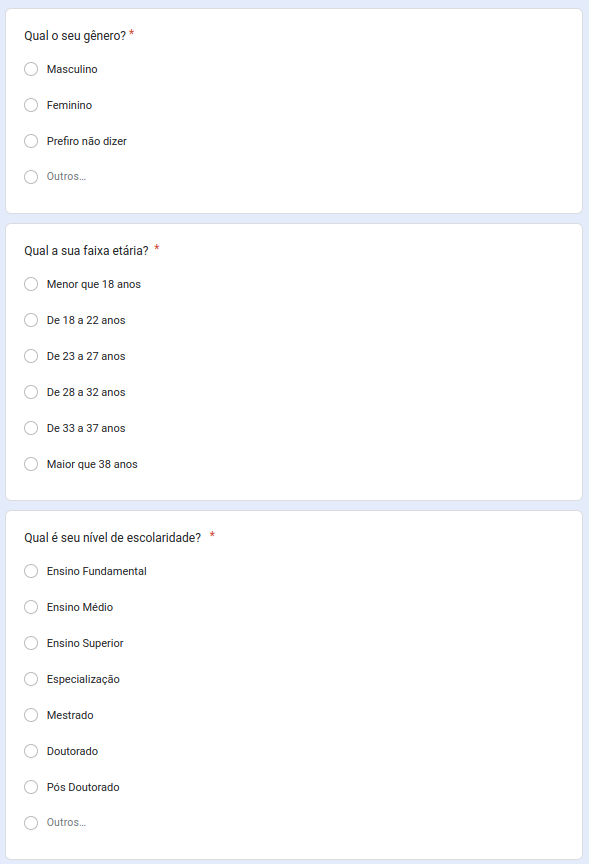
\includegraphics[scale=0.8]{figs/Form/01.png}
	\end{center}
	\caption{\label{AP_P01}Formulário de pesquisa com ambos participantes - Parte 1}
\end{figure}

\newpage

\begin{figure}[!h]
	\begin{center}
	    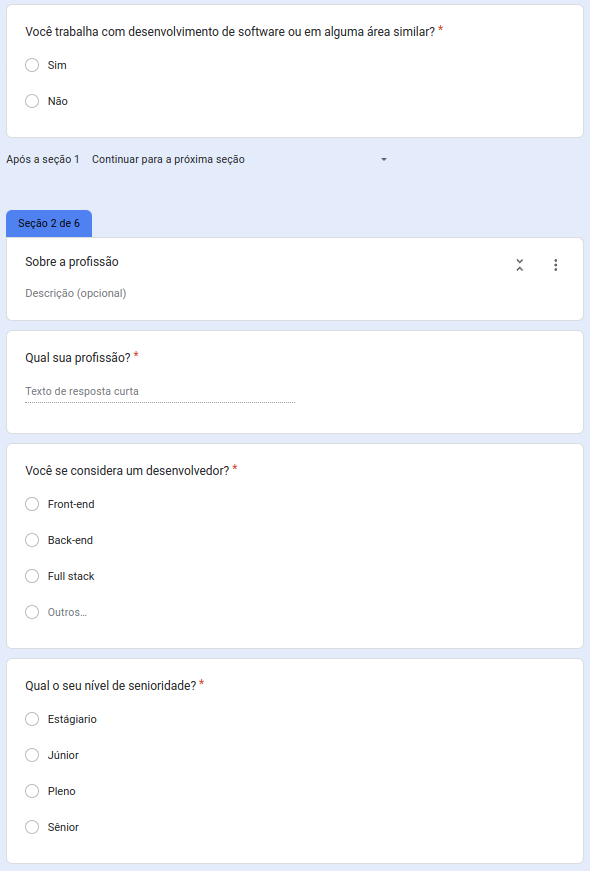
\includegraphics[scale=0.6]{figs/Form/02.png}
	\end{center}
	\caption{\label{AP_PPr}Formulário de pesquisa apenas \textbf{profissionais} - Parte Profissionais}
\end{figure}

\newpage

\begin{figure}[!h]
	\begin{center}
	    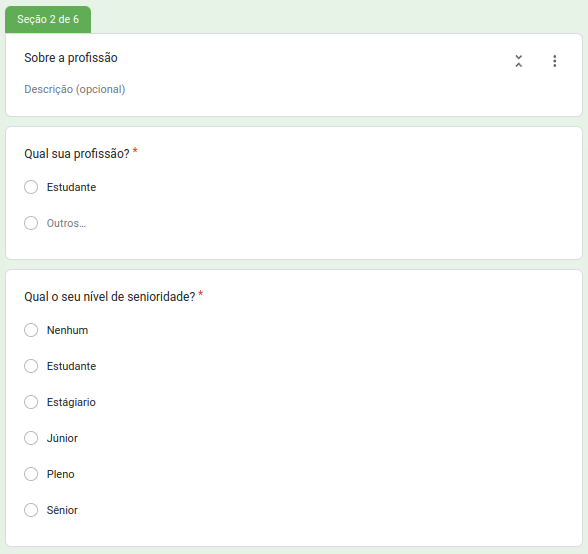
\includegraphics[scale=0.6]{figs/Form/03.png}
	\end{center}
	\caption{\label{AP_PEs}Formulário de pesquisa apenas \textbf{estudantes} - Parte Estudantes}
\end{figure}

\begin{figure}[!h]
	\begin{center}
	    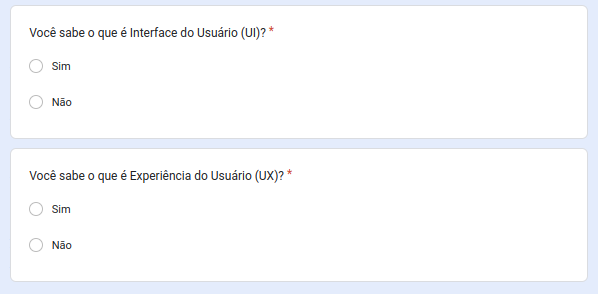
\includegraphics[scale=0.6]{figs/Form/04.png}
	\end{center}
	\caption{\label{AP_P02}Formulário de pesquisa com ambos participantes - Parte 2}
\end{figure}

\newpage

\section{Questionário}

Nas subseções a seguir todas as perguntas presentes nas Figuras são destinadas a ambos os grupos.

\subsection{Tela de Login}

As Figuras \ref{AP_LP01}, \ref{AP_LP02}, \ref{AP_LP03}, \ref{AP_LP04} referem-se à tela de login.

\begin{figure}[!h]
	\begin{center}
	    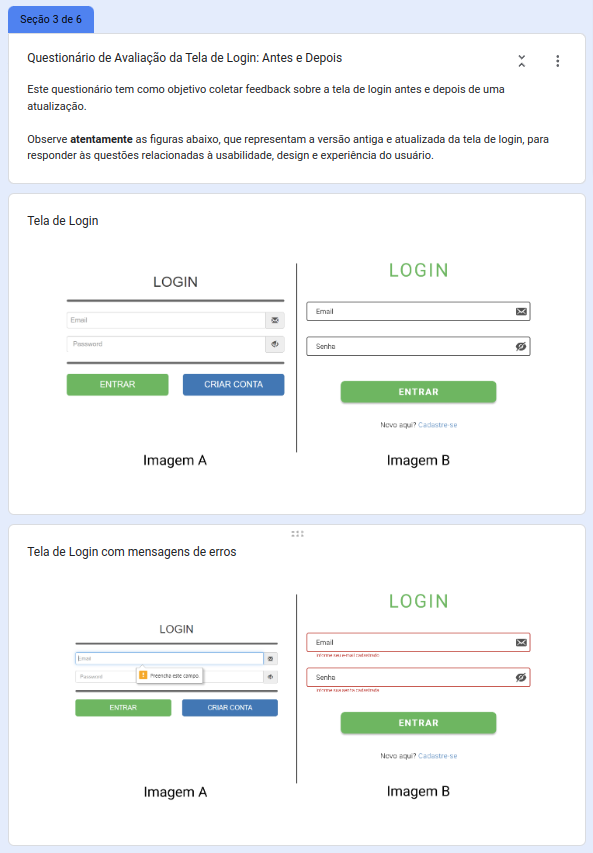
\includegraphics[scale=0.6]{figs/Form/05.png}
	\end{center}
	\caption{\label{AP_LP01}Formulário de pesquisa, Login - Parte 1}
\end{figure}

\newpage

\begin{figure}[!h]
	\begin{center}
	    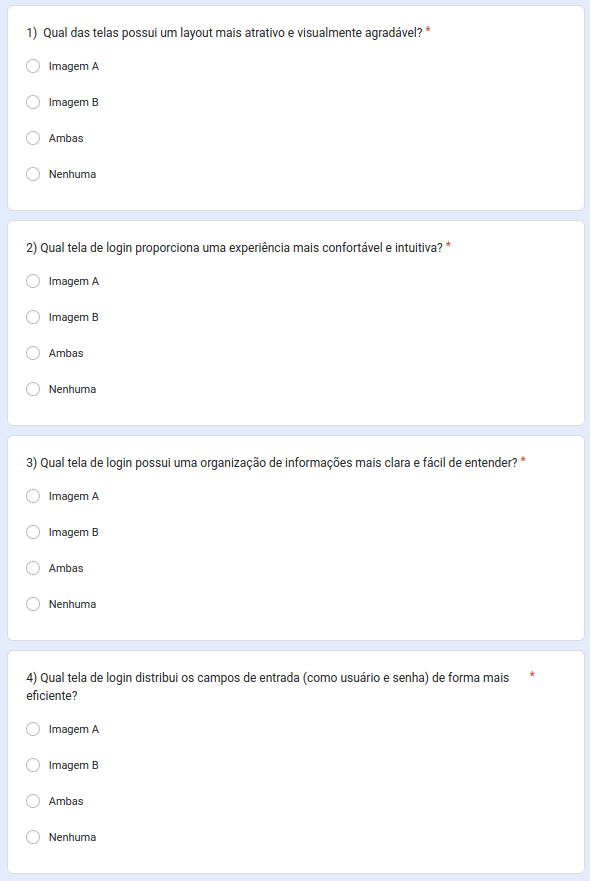
\includegraphics[scale=0.6]{figs/Form/06.png}
	\end{center}
	\caption{\label{AP_LP02}Formulário de pesquisa, Login - Parte 2}
\end{figure}

\newpage

\begin{figure}[!h]
	\begin{center}
	    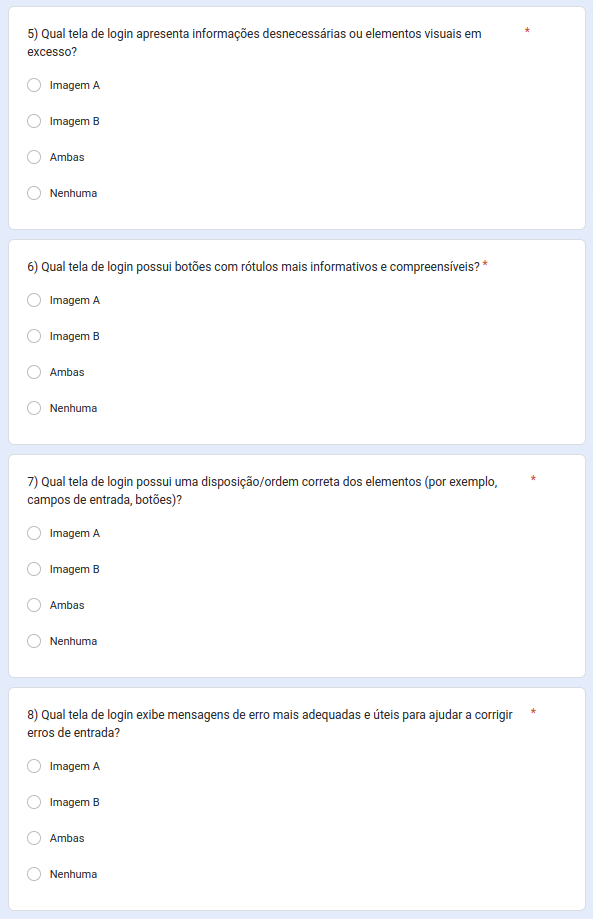
\includegraphics[scale=0.6]{figs/Form/07.png}
	\end{center}
	\caption{\label{AP_LP03}Formulário de pesquisa, Login - Parte 3}
\end{figure}

\newpage

\begin{figure}[!h]
	\begin{center}
	    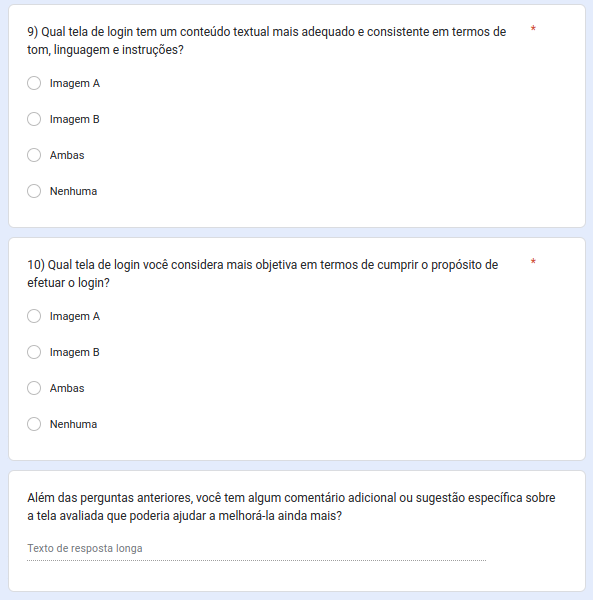
\includegraphics[scale=0.6]{figs/Form/08.png}
	\end{center}
	\caption{\label{AP_LP04}Formulário de pesquisa, Login - Parte 4}
\end{figure}

\newpage

\subsection{Tela de Cadastro}

As Figuras \ref{AP_CP01}, \ref{AP_CP02}, \ref{AP_CP03}, \ref{AP_CP04} referem-se à tela de cadastro.

\begin{figure}[!h]
	\begin{center}
	    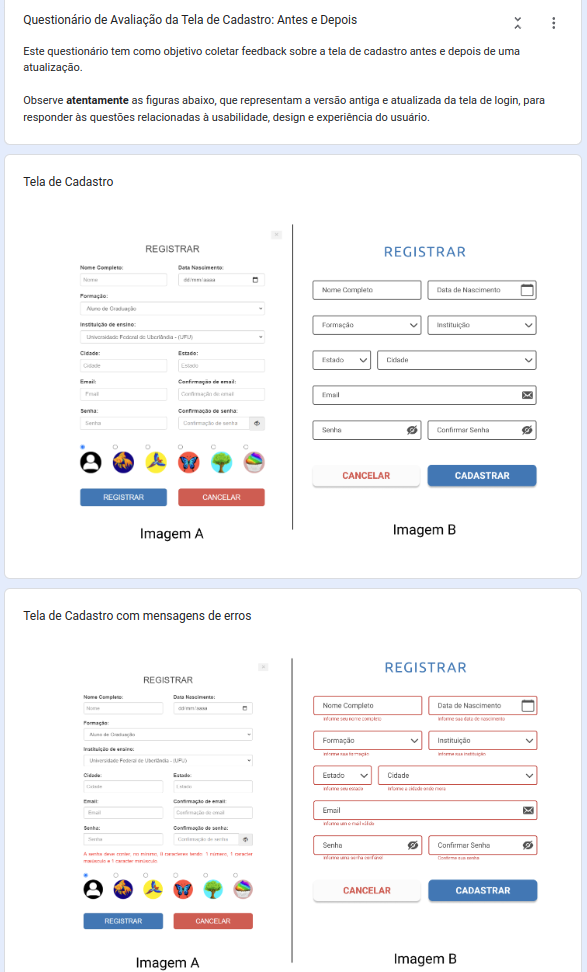
\includegraphics[scale=0.6]{figs/Form/09.png}
	\end{center}
	\caption{\label{AP_CP01}Formulário de pesquisa, Cadastro - Parte 1}
\end{figure}

\newpage

\begin{figure}[!h]
	\begin{center}
	    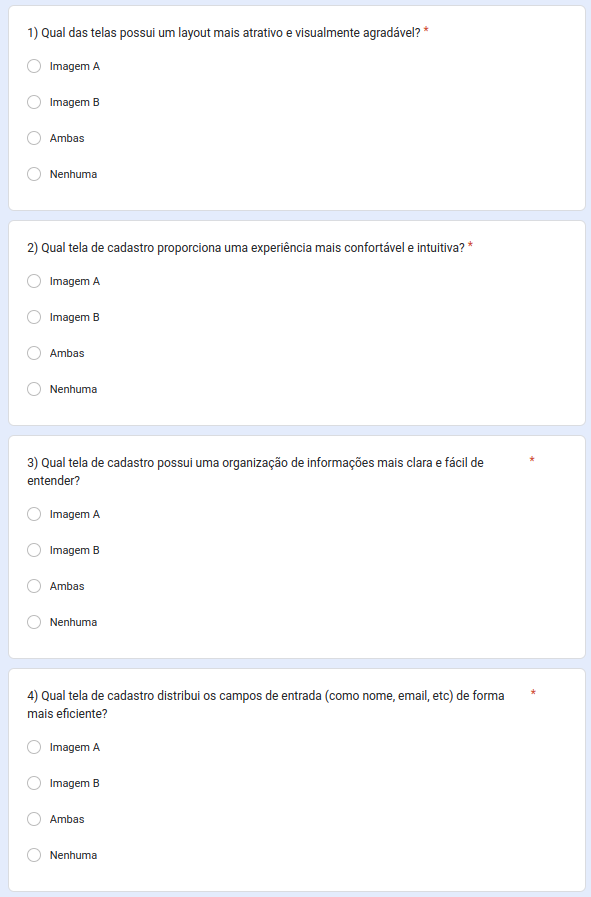
\includegraphics[scale=0.6]{figs/Form/10.png}
	\end{center}
	\caption{\label{AP_CP02}Formulário de pesquisa, Cadastro - Parte 2}
\end{figure}

\newpage

\begin{figure}[!h]
	\begin{center}
	    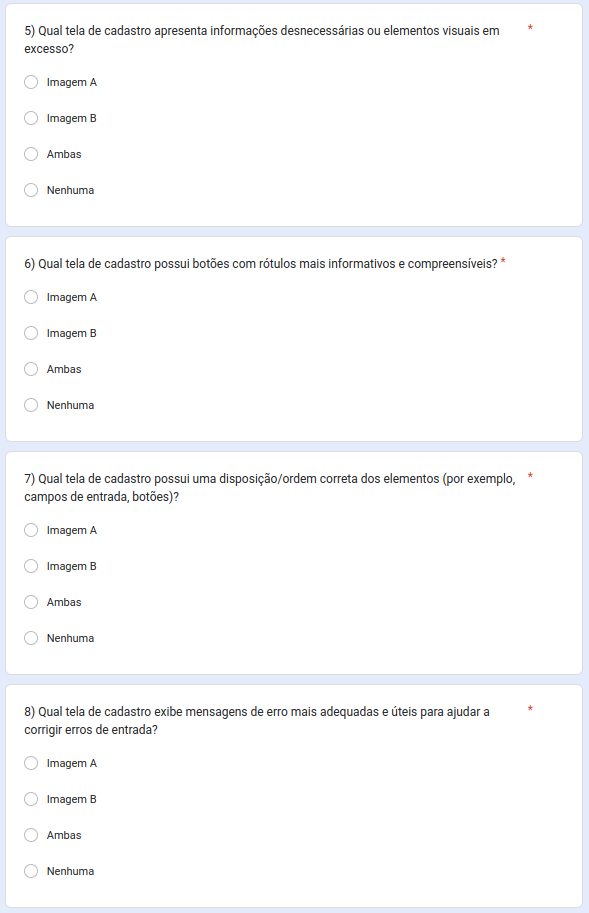
\includegraphics[scale=0.6]{figs/Form/11.png}
	\end{center}
	\caption{\label{AP_CP03}Formulário de pesquisa, Cadastro - Parte 3}
\end{figure}

\newpage

\begin{figure}[!h]
	\begin{center}
	    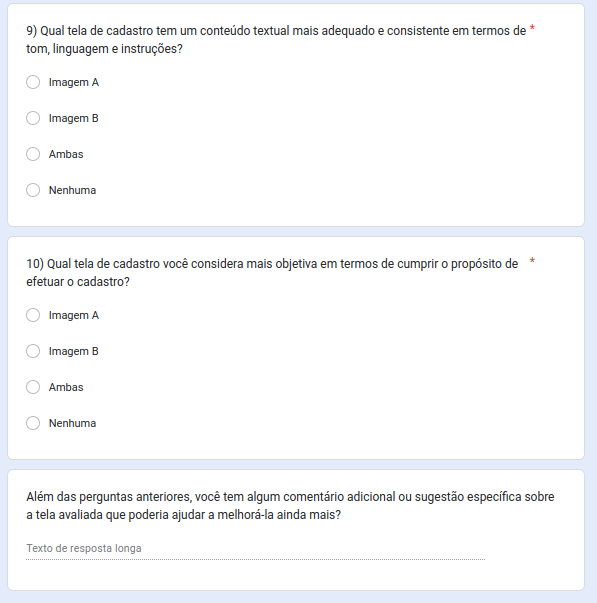
\includegraphics[scale=0.6]{figs/Form/12.png}
	\end{center}
	\caption{\label{AP_CP04}Formulário de pesquisa, Cadastro - Parte 4}
\end{figure}

\newpage

\subsection{Tela de Principal}

As Figuras \ref{AP_PP01}, \ref{AP_PP02}, \ref{AP_PP03}, \ref{AP_PP04}, \ref{AP_PP05}, \ref{AP_PP06} referem-se à tela de principal.

\begin{figure}[!h]
	\begin{center}
	    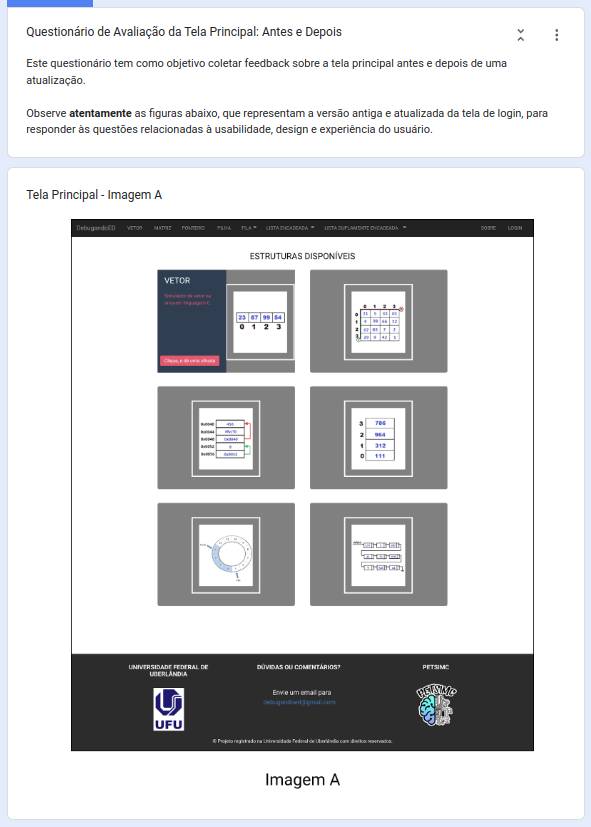
\includegraphics[scale=0.6]{figs/Form/13.png}
	\end{center}
	\caption{\label{AP_PP01}Formulário de pesquisa, Principal - Parte 1}
\end{figure}

\newpage

\begin{figure}[!h]
	\begin{center}
	    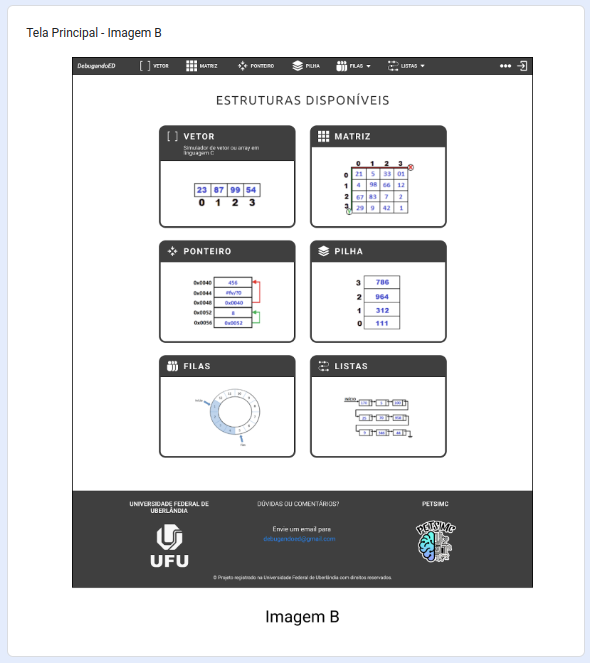
\includegraphics[scale=0.6]{figs/Form/14.png}
	\end{center}
	\caption{\label{AP_PP02}Formulário de pesquisa, Principal - Parte 2}
\end{figure}

\newpage

\begin{figure}[!h]
	\begin{center}
	    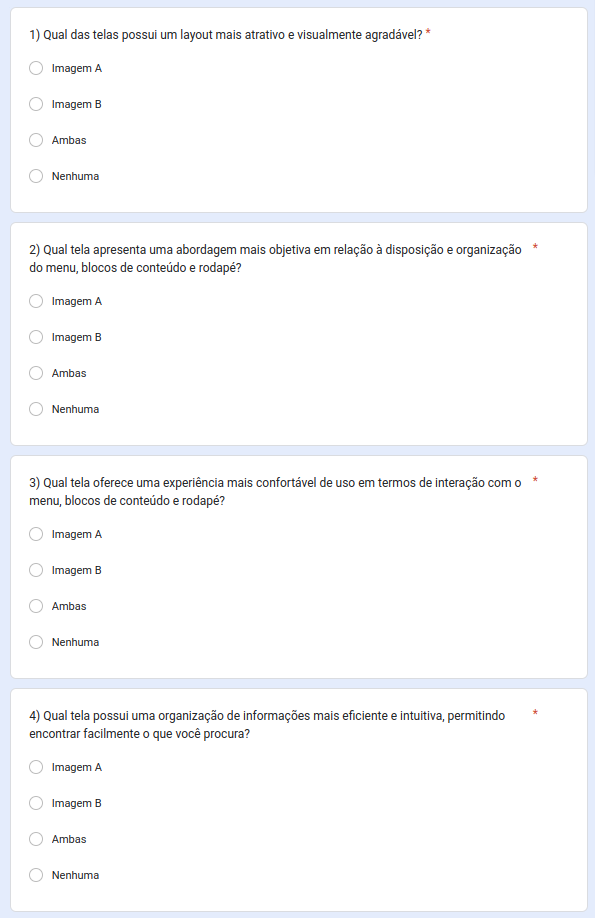
\includegraphics[scale=0.6]{figs/Form/15.png}
	\end{center}
	\caption{\label{AP_PP03}Formulário de pesquisa, Principal - Parte 3}
\end{figure}

\newpage

\begin{figure}[!h]
	\begin{center}
	    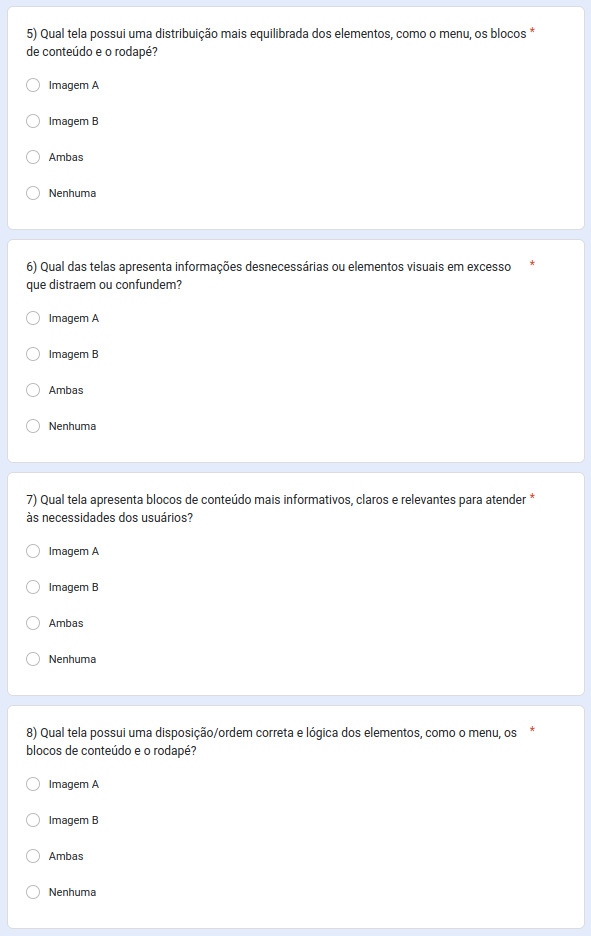
\includegraphics[scale=0.6]{figs/Form/16.png}
	\end{center}
	\caption{\label{AP_PP04}Formulário de pesquisa, Principal - Parte 4}
\end{figure}

\newpage

\begin{figure}[!h]
	\begin{center}
	    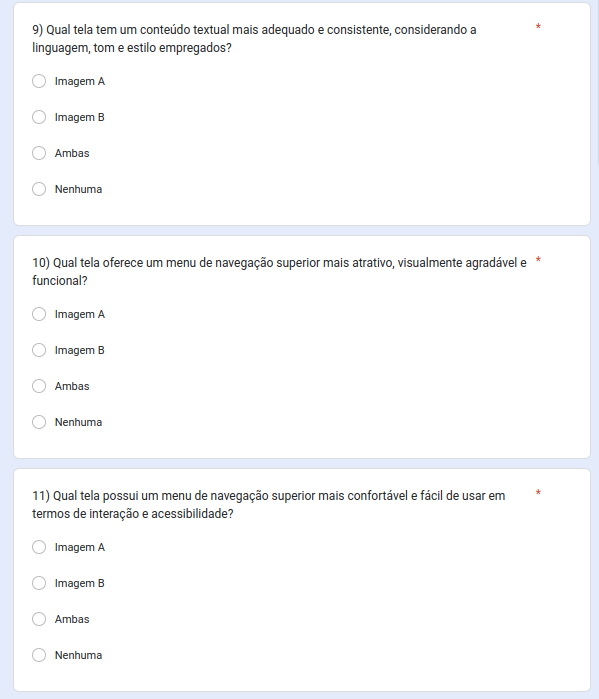
\includegraphics[scale=0.6]{figs/Form/17.png}
	\end{center}
	\caption{\label{AP_PP05}Formulário de pesquisa, Principal - Parte 5}
\end{figure}

\newpage

\begin{figure}[!h]
	\begin{center}
	    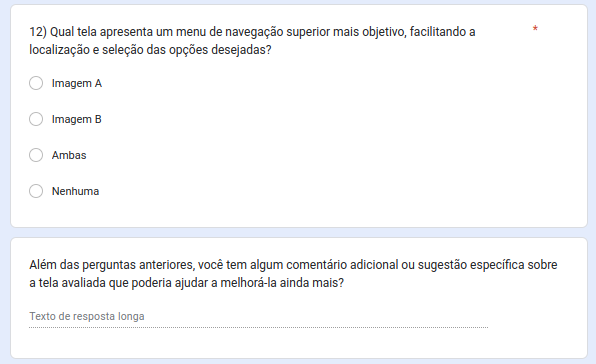
\includegraphics[scale=0.6]{figs/Form/18.png}
	\end{center}
	\caption{\label{AP_PP06}Formulário de pesquisa, Principal - Parte 6}
\end{figure}

\newpage

\subsection{Tela de Ponteiro}

As Figuras \ref{AP_PonP01}, \ref{AP_PonP02}, \ref{AP_PonP03}, \ref{AP_PonP04} referem-se à tela de ponteiro.

\begin{figure}[!h]
	\begin{center}
	    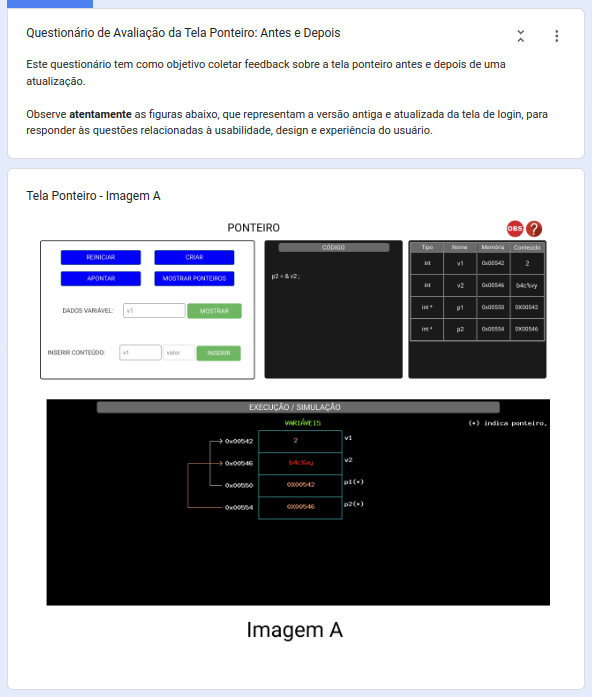
\includegraphics[scale=0.6]{figs/Form/19.png}
	\end{center}
	\caption{\label{AP_PonP01}Formulário de pesquisa, Ponteiro - Parte 1}
\end{figure}

\newpage

\begin{figure}[!h]
	\begin{center}
	    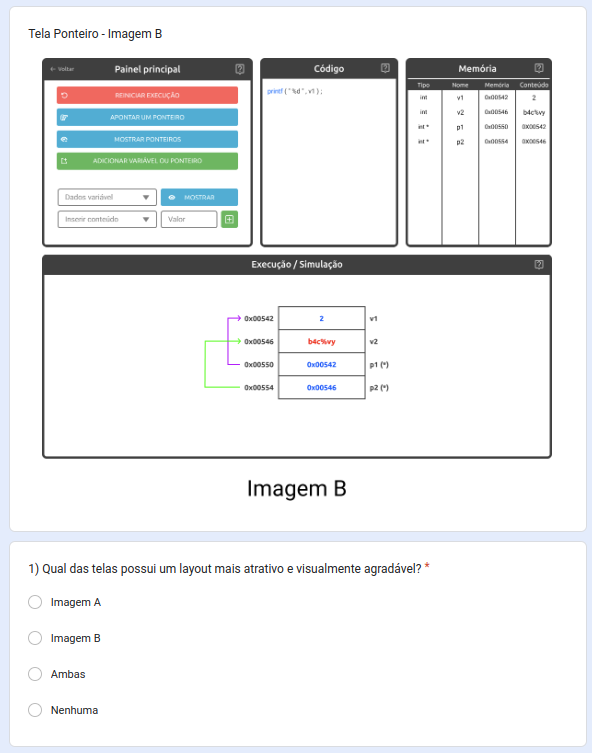
\includegraphics[scale=0.6]{figs/Form/20.png}
	\end{center}
	\caption{\label{AP_PonP02}Formulário de pesquisa, Ponteiro - Parte 2}
\end{figure}

\newpage

\begin{figure}[!h]
	\begin{center}
	    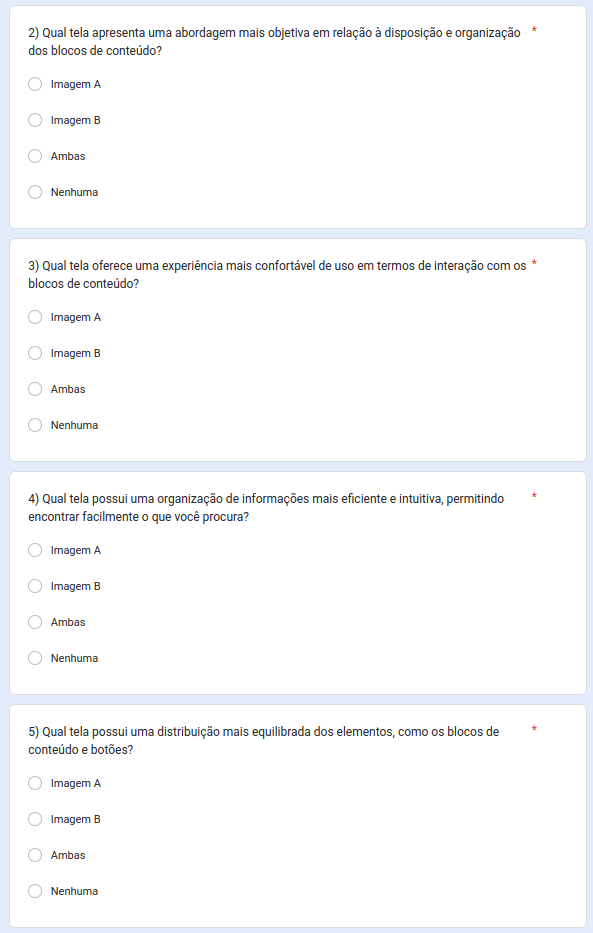
\includegraphics[scale=0.6]{figs/Form/21.png}
	\end{center}
	\caption{\label{AP_PonP03}Formulário de pesquisa, Ponteiro - Parte 3}
\end{figure}

\newpage

\begin{figure}[!h]
	\begin{center}
	    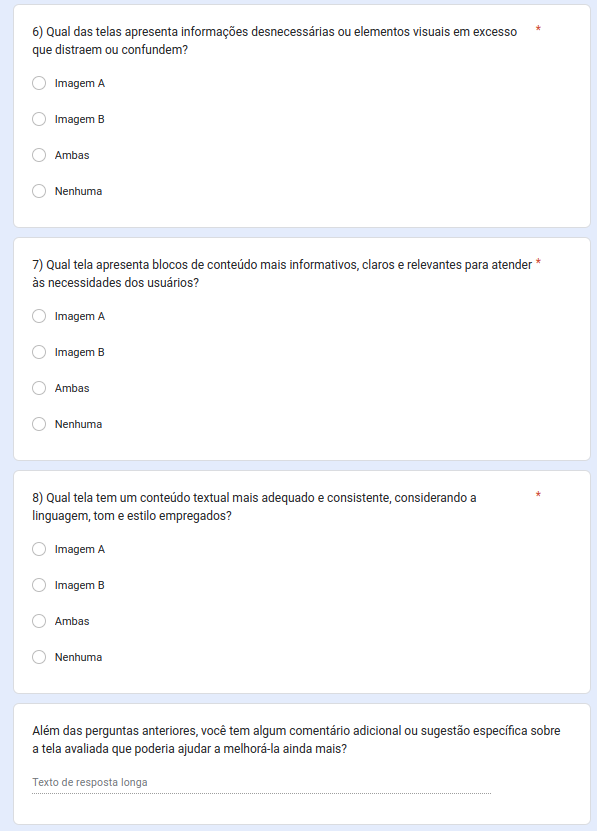
\includegraphics[scale=0.6]{figs/Form/22.png}
	\end{center}
	\caption{\label{AP_PonP04}Formulário de pesquisa, Ponteiro - Parte 4}
\end{figure}

		\chapter{Respostas dos estudantes}\label{respostas_dos_estudantes}

Este apêndice apresenta as respostas obtidas dos estudantes por meio do questionário aplicado durante a pesquisa. 

Este apêndice serve como um complemento vital ao corpo principal do trabalho, proporcionando aos leitores uma oportunidade de explorar, de forma mais tangível, a riqueza de dados qualitativos coletados durante a pesquisa.

\newpage

\section{Demográfico}

As Figuras \ref{APB_01}, \ref{APB_02}, \ref{APB_03} referem-se sobre os participantes.

\begin{figure}[!h]
	\begin{center}
	    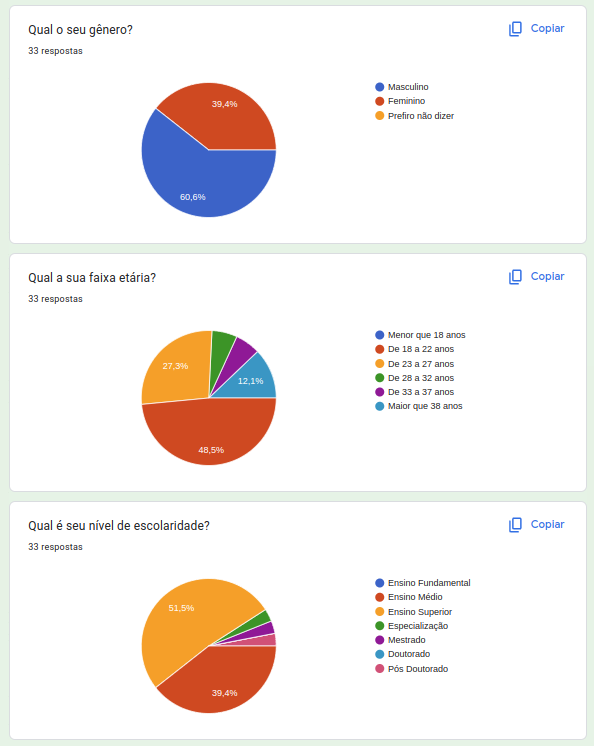
\includegraphics[scale=0.7]{figs/Answers/Students/01.png}
	\end{center}
	\caption{\label{APB_01}Respostas sobre os estudantes - Parte 1}
\end{figure}

\newpage

\begin{figure}[!h]
	\begin{center}
	    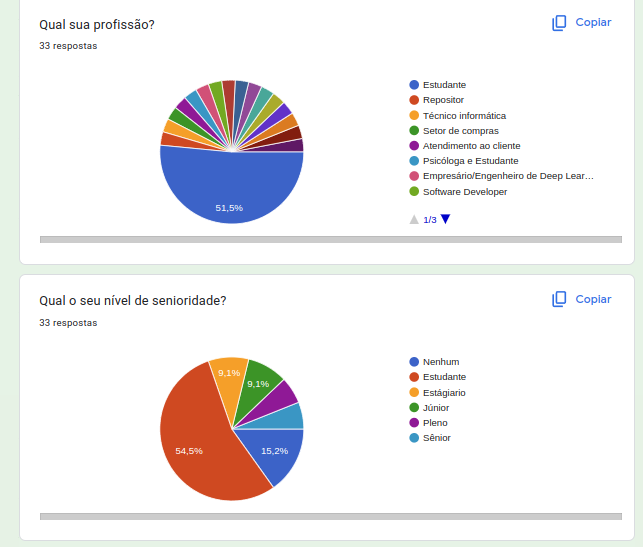
\includegraphics[scale=0.5]{figs/Answers/Students/02.png}
	\end{center}
	\caption{\label{APB_02}Respostas sobre os estudantes - Parte 2}
\end{figure}

\begin{figure}[!h]
	\begin{center}
	    \includegraphics[scale=0.5]{figs/Answers/Students/03.png}
	\end{center}
	\caption{\label{APB_03}Respostas sobre os estudantes - Parte 3}
\end{figure}

\newpage

\section{Tela de Login}

As Figuras \ref{APB_TL01}, \ref{APB_TL02}, \ref{APB_TL03}, \ref{APB_TL04} referem-se às respostas da primeira parte do questionário, na qual trata-se da avaliação da Tela de Login.

\begin{figure}[!h]
	\begin{center}
	    \includegraphics[scale=0.7]{figs/Answers/Students/04.png}
	\end{center}
	\caption{\label{APB_TL01}Respostas sobre a tela de login - Parte 1}
\end{figure}

\newpage

\begin{figure}[!h]
	\begin{center}
	    \includegraphics[scale=0.7]{figs/Answers/Students/05.png}
	\end{center}
	\caption{\label{APB_TL02}Respostas sobre a tela de login - Parte 2}
\end{figure}

\newpage

\begin{figure}[!h]
	\begin{center}
	    \includegraphics[scale=0.7]{figs/Answers/Students/06.png}
	\end{center}
	\caption{\label{APB_TL03}Respostas sobre a tela de login - Parte 3}
\end{figure}

\newpage

\begin{figure}[!h]
	\begin{center}
	    \includegraphics[scale=0.7]{figs/Answers/Students/07.png}
	\end{center}
	\caption{\label{APB_TL04}Respostas sobre a tela de login - Parte 4}
\end{figure}

\newpage

\section{Tela de Cadastro}

As Figuras \ref{APB_TC01}, \ref{APB_TC02}, \ref{APB_TC03}, \ref{APB_TC04} referem-se às respostas da segunda parte do questionário, na qual trata-se da avaliação da Tela de Cadastro.

\begin{figure}[!h]
	\begin{center}
	    \includegraphics[scale=0.7]{figs/Answers/Students/08.png}
	\end{center}
	\caption{\label{APB_TC01}Respostas sobre a tela de cadastro - Parte 1}
\end{figure}

\newpage

\begin{figure}[!h]
	\begin{center}
	    \includegraphics[scale=0.7]{figs/Answers/Students/09.png}
	\end{center}
	\caption{\label{APB_TC02}Respostas sobre a tela de cadastro - Parte 2}
\end{figure}

\newpage

\begin{figure}[!h]
	\begin{center}
	    \includegraphics[scale=0.7]{figs/Answers/Students/10.png}
	\end{center}
	\caption{\label{APB_TC03}Respostas sobre a tela de cadastro - Parte 3}
\end{figure}

\newpage

\begin{figure}[!h]
	\begin{center}
	    \includegraphics[scale=0.7]{figs/Answers/Students/11.png}
	\end{center}
	\caption{\label{APB_TC04}Respostas sobre a tela de cadastro - Parte 4}
\end{figure}

\newpage

\section{Tela Principal}

As Figuras \ref{APB_TP01}, \ref{APB_TP02}, \ref{APB_TP03}, \ref{APB_TP04}, \ref{APB_TP05} referem-se às respostas da terceira parte do questionário, na qual trata-se da avaliação da Tela Principal.

\begin{figure}[!h]
	\begin{center}
	    \includegraphics[scale=0.7]{figs/Answers/Students/12.png}
	\end{center}
	\caption{\label{APB_TP01}Respostas sobre a tela principal - Parte 1}
\end{figure}

\newpage

\begin{figure}[!h]
	\begin{center}
	    \includegraphics[scale=0.7]{figs/Answers/Students/13.png}
	\end{center}
	\caption{\label{APB_TP02}Respostas sobre a tela principal - Parte 2}
\end{figure}

\newpage

\begin{figure}[!h]
	\begin{center}
	    \includegraphics[scale=0.7]{figs/Answers/Students/14.png}
	\end{center}
	\caption{\label{APB_TP03}Respostas sobre a tela principal - Parte 3}
\end{figure}

\newpage

\begin{figure}[!h]
	\begin{center}
	    \includegraphics[scale=0.5]{figs/Answers/Students/15.png}
	\end{center}
	\caption{\label{APB_TP04}Respostas sobre a tela principal - Parte 4}
\end{figure}


\begin{figure}[!h]
	\begin{center}
	    \includegraphics[scale=0.5]{figs/Answers/Students/16.png}
	\end{center}
	\caption{\label{APB_TP05}Respostas sobre a tela principal - Parte 5}
\end{figure}

\newpage

\section{Tela do Ponteiro}

As Figuras \ref{APB_TPon01}, \ref{APB_TPon02}, \ref{APB_TPon03} referem-se às respostas da terceira parte do questionário, na qual trata-se da avaliação da Tela do Ponteiro.

\begin{figure}[!h]
	\begin{center}
	    \includegraphics[scale=0.7]{figs/Answers/Students/17.png}
	\end{center}
	\caption{\label{APB_TPon01}Respostas sobre a tela do ponteiro - Parte 1}
\end{figure}

\newpage

\begin{figure}[!h]
	\begin{center}
	    \includegraphics[scale=0.7]{figs/Answers/Students/18.png}
	\end{center}
	\caption{\label{APB_TPon02}Respostas sobre a tela do ponteiro - Parte 2}
\end{figure}

\newpage

\begin{figure}[!h]
	\begin{center}
	    \includegraphics[scale=0.7]{figs/Answers/Students/19.png}
	\end{center}
	\caption{\label{APB_TPon03}Respostas sobre a tela do ponteiro - Parte 3}
\end{figure}

\newpage
		\chapter{Respostas dos Profissionais}\label{respostas_dos_profissionais}

Este apêndice apresenta as respostas obtidas apenas dos profissionais da areá de tecnologia por meio do questionário aplicado durante a pesquisa. 

Este apêndice serve como um complemento vital ao corpo principal do trabalho, proporcionando aos leitores uma oportunidade de explorar, de forma mais tangível, a riqueza de dados qualitativos coletados durante a pesquisa.

\newpage

\section{Demográfico}

As Figuras \ref{APC_01}, \ref{APC_02}, \ref{APC_03} referem-se sobre os participantes.

\begin{figure}[!h]
	\begin{center}
	    \includegraphics[scale=0.7]{figs/Answers/Professionals/01.png}
	\end{center}
	\caption{\label{APC_01}Respostas sobre os profissionais - Parte 1}
\end{figure}

\newpage

\begin{figure}[!h]
	\begin{center}
	    \includegraphics[scale=0.7]{figs/Answers/Professionals/02.png}
	\end{center}
	\caption{\label{APC_02}Respostas sobre os profissionais - Parte 2}
\end{figure}

\newpage

\begin{figure}[!h]
	\begin{center}
	    \includegraphics[scale=0.7]{figs/Answers/Professionals/03.png}
	\end{center}
	\caption{\label{APC_03}Respostas sobre os profissionais - Parte 3}
\end{figure}

\newpage

\section{Tela de Login}

As Figuras \ref{APC_TL01}, \ref{APC_TL02}, \ref{APC_TL03}, \ref{APC_TL04} referem-se às respostas da primeira parte do questionário, na qual trata-se da avaliação da Tela de Login.

\begin{figure}[!h]
	\begin{center}
	    \includegraphics[scale=0.7]{figs/Answers/Professionals/04.png}
	\end{center}
	\caption{\label{APC_TL01}Respostas sobre a tela de login - Parte 1}
\end{figure}

\newpage

\begin{figure}[!h]
	\begin{center}
	    \includegraphics[scale=0.7]{figs/Answers/Professionals/05.png}
	\end{center}
	\caption{\label{APC_TL02}Respostas sobre a tela de login - Parte 2}
\end{figure}

\newpage

\begin{figure}[!h]
	\begin{center}
	    \includegraphics[scale=0.7]{figs/Answers/Professionals/06.png}
	\end{center}
	\caption{\label{APC_TL03}Respostas sobre a tela de login - Parte 3}
\end{figure}

\newpage

\begin{figure}[!h]
	\begin{center}
	    \includegraphics[scale=0.7]{figs/Answers/Professionals/07.png}
	\end{center}
	\caption{\label{APC_TL04}Respostas sobre a tela de login - Parte 4}
\end{figure}

\newpage

\section{Tela de Cadastro}

As Figuras \ref{APC_TC01}, \ref{APC_TC02}, \ref{APC_TC03}, \ref{APC_TC04} referem-se às respostas da segunda parte do questionário, na qual trata-se da avaliação da Tela de Cadastro.

\begin{figure}[!h]
	\begin{center}
	    \includegraphics[scale=0.7]{figs/Answers/Professionals/08.png}
	\end{center}
	\caption{\label{APC_TC01}Respostas sobre a tela de cadastro - Parte 1}
\end{figure}

\newpage

\begin{figure}[!h]
	\begin{center}
	    \includegraphics[scale=0.7]{figs/Answers/Professionals/09.png}
	\end{center}
	\caption{\label{APC_TC02}Respostas sobre a tela de cadastro - Parte 2}
\end{figure}

\newpage

\begin{figure}[!h]
	\begin{center}
	    \includegraphics[scale=0.7]{figs/Answers/Professionals/10.png}
	\end{center}
	\caption{\label{APC_TC03}Respostas sobre a tela de cadastro - Parte 3}
\end{figure}

\newpage

\begin{figure}[!h]
	\begin{center}
	    \includegraphics[scale=0.7]{figs/Answers/Professionals/11.png}
	\end{center}
	\caption{\label{APC_TC04}Respostas sobre a tela de cadastro - Parte 4}
\end{figure}

\newpage

\section{Tela Principal}

As Figuras \ref{APC_TP01}, \ref{APC_TP02}, \ref{APC_TP03}, \ref{APC_TP04}, \ref{APC_TP05} referem-se às respostas da terceira parte do questionário, na qual trata-se da avaliação da Tela Principal.

\begin{figure}[!h]
	\begin{center}
	    \includegraphics[scale=0.7]{figs/Answers/Professionals/12.png}
	\end{center}
	\caption{\label{APC_TP01}Respostas sobre a tela principal - Parte 1}
\end{figure}

\newpage

\begin{figure}[!h]
	\begin{center}
	    \includegraphics[scale=0.7]{figs/Answers/Professionals/13.png}
	\end{center}
	\caption{\label{APC_TP02}Respostas sobre a tela principal - Parte 2}
\end{figure}

\newpage

\begin{figure}[!h]
	\begin{center}
	    \includegraphics[scale=0.7]{figs/Answers/Professionals/14.png}
	\end{center}
	\caption{\label{APC_TP03}Respostas sobre a tela principal - Parte 3}
\end{figure}

\newpage

\begin{figure}[!h]
	\begin{center}
	    \includegraphics[scale=0.6]{figs/Answers/Professionals/15.png}
	\end{center}
	\caption{\label{APC_TP04}Respostas sobre a tela principal - Parte 4}
\end{figure}


\begin{figure}[!h]
	\begin{center}
	    \includegraphics[scale=0.5]{figs/Answers/Professionals/16.png}
	\end{center}
	\caption{\label{APC_TP05}Respostas sobre a tela principal - Parte 5}
\end{figure}

\newpage

\section{Tela do Ponteiro}

As Figuras \ref{APC_TPon01}, \ref{APC_TPon02}, \ref{APC_TPon03} referem-se às respostas da terceira parte do questionário, na qual trata-se da avaliação da Tela do Ponteiro.

\begin{figure}[!h]
	\begin{center}
	    \includegraphics[scale=0.7]{figs/Answers/Professionals/17.png}
	\end{center}
	\caption{\label{APC_TPon01}Respostas sobre a tela do ponteiro - Parte 1}
\end{figure}

\newpage

\begin{figure}[!h]
	\begin{center}
	    \includegraphics[scale=0.7]{figs/Answers/Professionals/18.png}
	\end{center}
	\caption{\label{APC_TPon02}Respostas sobre a tela do ponteiro - Parte 2}
\end{figure}

\newpage

\begin{figure}[!h]
	\begin{center}
	    \includegraphics[scale=0.7]{figs/Answers/Professionals/19.png}
	\end{center}
	\caption{\label{APC_TPon03}Respostas sobre a tela do ponteiro - Parte 3}
\end{figure}

\newpage
		
	\end{apendicesenv}
	% ---	
	
\end{document}